%%%%%%%%%%%%%%%%%%%%%%%%%%%%%%%%%%%%%%%%%%%%%%%%%%%%%%%%%%%%%%%
%
% Welcome to Overleaf --- just edit your LaTeX on the left,
% and we'll compile it for you on the right. If you open the
% 'Share' menu, you can invite other users to edit at the same
% time. See www.overleaf.com/learn for more info. Enjoy!
%
%%%%%%%%%%%%%%%%%%%%%%%%%%%%%%%%%%%%%%%%%%%%%%%%%%%%%%%%%%%%%%%
\documentclass[12pt,a4paper,oneside]{book}


\input{Packages}


%\makenoidxglossaries 

%\newglossaryentry{latex}
%{
       % name=latex,
        %description={Is a mark up language specially suited for scientific documents}
%}



%\selectlanguage{English}



\hypersetup{
    colorlinks=true,
    linkcolor=black,
    filecolor=magenta,      
    urlcolor=cyan,
    pdfauthor={Name},  %put your name here
    pdftitle={PDF_TTILE},  %PDF title
    pdfpagemode=FullScreen,
    }



\begin{document}



\definecolor{codegreen}{rgb}{0,0.6,0}
    \definecolor{codegray}{rgb}{0.5,0.5,0.5}
    \definecolor{codepurple}{rgb}{0.58,0,0.82}
    \definecolor{backcolour}{rgb}{0.95,0.95,0.92}
    
    \lstdefinestyle{mystyle}{
        backgroundcolor=\color{backcolour},   
        keywordstyle=\color{magenta},
        numberstyle=\tiny\color{codegreen},
        stringstyle=\color{codepurple},
        basicstyle=\ttfamily\footnotesize,
        breakatwhitespace=false,         
        breaklines=true,                 
        captionpos=b,                    
        keepspaces=true,                 
        numbers=left,                    
        numbersep=5pt,                  
        showspaces=false,                
        showstringspaces=false,
        showtabs=false,                  
        tabsize=2
    }




%
\thispagestyle{empty}

\includegraphics[height=2cm]{Logos/UTM.png} 
         \hfill

\includegraphics[height=2cm]{Logos/fst.png}
        
\vspace{0.9cm}
\begin{center}
{\large \textsc{\textbf{Mémoire du projet de fin d'études}}}\\[0.1cm]
{\large \textsc{Pour L'obtention du Diplôme d'Ingénieur d'État}}\\[0.1cm]
{\large \textsc{\textit{Filière: Génie Informatique}}} \\[0.05cm] 
\vspace{-0.04cm}
% Title
\rule{\linewidth}{0.3mm} \\[0.4cm]   % à ajuster l'éspace en cas de besoin: [1cm]
 { \huge \textbf{ STM32Cube Competitor Benchmark }} \\[0.15cm] 
\rule{\linewidth}{0.3mm} \\[0.4cm]
\vspace{0.4cm}


\includegraphics[width=4cm]{Logos/STMicroelectronics.png}  % STMicroelectronics company logo

\vspace{1cm}

% Author and supervisor
\noindent
\begin{minipage}{0.9\textwidth}
    \vspace{-7mm}
  \begin{flushleft} \large
    \emph{Réalisé par :}\\
    M. Fares \textsc{Dkhili} %\& Mme / M. Xxxx \textsc{XXXX}  %Au cas de binôme, remove the % \\
  \end{flushleft}
\end{minipage}
\begin{minipage}{0.4\textwidth}

\end{minipage}\\[0.6cm]

{\large \textit{Soutenu en Septembre 2026, devant le jury composé de : }}\\[0.5cm]


\begin{tabular}{p{1cm}lll}
 & \large Mme. Anissa \textsc{Omrane}  & \large FST & \large - Présidente \\[0.1cm]
 & \large Mme. Sana \textsc{Younes}  & \large FST & \large - Examinatrice \\[0.1cm]
 & \large M. Aymen \textsc{Zemrani}  & \large FST & \large - Encadrant académique \\[0.1cm]
  & \large Mme. Sirine \textsc{Eljazi}  & \large STMicroelectronics & \large - Encadrante professionnelle \\[0.1cm]
 
\end{tabular}

\vspace{0.5cm}

\includegraphics[scale=0.6]{Logos/ZLAFA.png}


\textsc{Agence National de Réglementation des Télécommunications}\\
\textsc{Institut National des Postes et Télécommunications}
% Bottom of the page

%\vspace{0.3cm}
{\large Promotion : 2025/2026}
   
\end{center}


 %FRENCH ONE


\thispagestyle{empty}

\includegraphics[height=2cm]{Logos/UTM.png} 
         \hfill

\includegraphics[height=2cm]{Logos/fst.png}
        
\vspace{0.9cm}
\begin{center}
{\large \textsc{\textbf{Thesis of the end-of-study project}}}\\[0.1cm]
{\large \textsc{To obtain the State Engineering Diploma}}\\[0.1cm]
{\large \textsc{\textit{Major: Computer Engineering}}} \\[0.05cm] 
\vspace{-0.04cm}
% Title
\rule{\linewidth}{0.3mm} \\[0.4cm]   % à ajuster l'éspace en cas de besoin: [1cm]
 { \huge \textbf{ STM32Cube Competitor Benchmark }} \\[0.15cm] 
\rule{\linewidth}{0.3mm} \\[0.4cm]
\vspace{0.4cm}


\includegraphics[width=4cm]{Logos/STMicroelectronics.png}  % STMicroelectronics company logo

\vspace{1cm}

% Author and supervisor
\noindent
\begin{minipage}{0.9\textwidth}
    \vspace{-7mm}
  \begin{flushleft} \large
    \emph{Authored by :}\\
    Fares \textsc{Dkhili} %\& Mr/Mrs/Ms. Xxxx \textsc{XXXX}  %Au cas de binôme, remove the % \\
  \end{flushleft}
\end{minipage}
\begin{minipage}{0.4\textwidth}

\end{minipage}\\[0.6cm]

{\large \textit{Defended on September 2026, before the jury composed of :}}\\[0.5cm]


\begin{tabular}{p{1cm}lll}
 & \large Mrs. Anissa \textsc{Omrane}  & \large FST & \large - President \\[0.1cm]
 & \large Mrs. Sana \textsc{Younes}  & \large FST & \large - Examiner \\[0.1cm]
 & \large Mr. Aymen \textsc{Zemrani}  & \large FST & \large - Academic supervisor \\[0.1cm]
  & \large Mrs. Sirine \textsc{Eljazi}  & \large STMicroelectronics & \large - Professional supervisor \\[0.1cm]
 
\end{tabular}

\vspace{0.5cm}


% Bottom of the page

%\vspace{0.3cm}
{\large Class of : 2025/2026}
   
\end{center}


 % ENGLISH

\afterpage{\blankpage}  %page vide obligatoire

\frontmatter


\chapter*{Dedicated to}
\addcontentsline{toc}{chapter}{Dedication}

  \begin{dedication}
  
    To my dear parents, whose unconditional love, patience, and countless
    sacrifices have carried me to this moment. Everything I have achieved is
    a reflection of the values you taught me.
    
    \par   %% or a blank line
    \vspace{1\baselineskip}
    
    To my family and my friends, who never stopped believing in me and who
    lifted me through every doubt and every long night. This work is as much
    yours as it is mine.

    \vspace{\baselineskip}
    \usefont{T1}{LobsterTwo-LF}{bx}{it} Fares Dkhili.
  \end{dedication}





\chapter*{Acknowledgments}
\addcontentsline{toc}{chapter}{Acknowledgments}

This project marks the end of my engineering studies, and it could not have
come together without the people who guided and supported me along the way.

I am deeply grateful to Ms. Sirine Eljazi, my supervisor at STMicroelectronics,
for her trust, her availability, and the technical insight she shared throughout
this work. Her guidance shaped both the project and the engineer I have become.
I also thank the entire STMicroelectronics team for the warm welcome and for
making my time within the company a genuine learning experience.

I would like to express my sincere thanks to Mr. Aymen Zemrani, my academic
supervisor at the Faculty of Sciences of Tunis (FST), for his rigorous
follow-up, his sound advice, and his constant encouragement from the first day
to the last.

My thanks also go to the members of the jury: to Ms. Anissa Omrane for the
honor of chairing the jury, and to Ms. Sana Younes for accepting to examine
and evaluate this work. Their time and attention are sincerely appreciated.

I extend my gratitude to the teaching staff of the Faculty of Sciences of
Tunis at the University of Tunis El Manar, whose dedication over these years
laid the foundations on which this project was built.

Finally, my heartfelt thanks to my family and friends, whose unwavering
support and patience accompanied me through every stage of this journey.


\chapter*{Résumé}
\addcontentsline{toc}{chapter}{Résumé}


Ce rapport présente les travaux réalisés dans le cadre d'un projet de fin d'études au sein de STMicroelectronics Tunis, portant sur le benchmarking de l'écosystème STM32Cube face aux écosystèmes concurrents (GigaDevice GD32, NXP, Texas Instruments, Renesas). L'objectif est de fournir à l'équipe de marketing technique des données comparatives objectives, reproductibles et interprétables sur l'empreinte mémoire (flash et RAM), les performances d'exécution et la maturité des piles logicielles embarquées.

Nous avons conçu une méthodologie de benchmarking structurée reposant sur des scénarios identiques exécutés sur les deux plateformes comparées, avec le même niveau d'optimisation, la même fréquence d'horloge et le même comportement observable. Deux outils complémentaires ont été développés en parallèle pour rendre cette méthodologie scalable et reproductible~: \emph{MCU Workflow Studio}, une application d'analyse d'empreinte firmware inter-vendeurs qui automatise la comparaison de fichiers linker map, la classification par couche architecturale et l'export des résultats~; et le \emph{MCU Benchmark Copilot Agent}, un système d'agents IA personnalisé intégré à VS~Code qui accélère la création, le portage et le débogage des benchmarks tout en imposant l'équivalence sémantique et l'équité des comparaisons.

Les résultats obtenus sur la comparaison ST~vs~GD32 --- couvrant la pile USB device (scénarios HID et CDC) et l'intégration FreeRTOS (scénarios basique, coopératif et préemptif) --- révèlent un compromis architectural clair~: STM32 consomme davantage de ROM (35--88\,\%) en raison de sa couche HAL modulaire, mais utilise significativement moins de RAM (57--65\,\% pour l'USB) et offre des performances d'initialisation supérieures (61,7\,\% plus rapide). Des propositions d'amélioration ciblées sont formulées, notamment l'optimisation du module HAL~RCC et la sélection fine des fonctionnalités USB à la compilation.

\noindent\rule[2pt]{\textwidth}{0.5pt}

{\textbf{Mots clés :}}
STM32Cube, benchmarking, empreinte mémoire, microcontrôleur, analyse de fichier linker map, FreeRTOS, USB, GD32, portage inter-vendeurs, agent IA.
\\
\noindent\rule[2pt]{\textwidth}{0.5pt}

% \cleardoublepage
%

\chapter*{Summary}
\addcontentsline{toc}{chapter}{Summary}


This report presents work carried out during an end-of-studies internship at STMicroelectronics Tunis, focused on benchmarking the STM32Cube ecosystem against competing vendor ecosystems (GigaDevice GD32, NXP, Texas Instruments, Renesas). The goal is to provide the technical marketing team with objective, reproducible, and interpretable comparative data on firmware memory footprint (flash and RAM), execution performance, and middleware maturity.

We designed a structured benchmarking methodology based on identical scenarios executed on both compared platforms under the same optimisation level, clock frequency, and observable behaviour. Two complementary tools were developed in parallel to make this methodology scalable and reproducible: \emph{MCU Workflow Studio}, a cross-vendor firmware footprint analysis application that automates linker-map comparison, architectural-layer classification, and result export; and the \emph{MCU Benchmark Copilot Agent}, a custom AI agent system integrated into VS~Code that accelerates benchmark creation, porting, and debugging while enforcing semantic equivalence and comparison fairness.

Results from the ST-versus-GD32 comparison --- covering the USB device stack (HID and CDC scenarios) and FreeRTOS integration (basic, cooperative, and preemptive scheduling scenarios) --- reveal a clear architectural trade-off: STM32 consumes more ROM (35--88\,\%) due to its modular HAL layer, but uses significantly less RAM (57--65\,\% for USB) and delivers superior initialisation performance (61.7\,\% faster). Targeted enhancement proposals are formulated, notably optimising the HAL~RCC module and enabling finer compile-time USB feature selection.

\noindent\rule[2pt]{\textwidth}{0.5pt}

{\textbf{Key Words:}}
STM32Cube, benchmarking, memory footprint, microcontroller, linker-map analysis, FreeRTOS, USB, GD32, cross-vendor porting, AI agent.
\\
\noindent\rule[2pt]{\textwidth}{0.5pt}

% \cleardoublepage
%

\chapter*{\RL{ملخص}}
\addcontentsline{toc}{chapter}{Arabic Abstract}

\begin{RLtext}

\noindent يقدّم هذا التقرير الأعمال المنجزة في إطار مشروع نهاية الدراسات بشركة إس تي مايكروإلكترونيكس بتونس، والتي تتمحور حول قياس أداء المنظومة البرمجية STM32Cube مقارنةً بالمنظومات المنافسة (GigaDevice GD32، NXP، Texas Instruments، Renesas). يهدف المشروع إلى تزويد فريق التسويق التقني ببيانات مقارنة موضوعية وقابلة للتكرار حول البصمة الذاكرية (فلاش وRAM) وأداء التنفيذ ونضج الطبقات البرمجية الوسيطة.

صمّمنا منهجية قياس أداء مهيكلة تعتمد على سيناريوهات متطابقة تُنفَّذ على كلتا المنصتين المقارنتين بنفس مستوى التحسين وتردد الساعة والسلوك الملاحظ. طوّرنا بالتوازي أداتين متكاملتين: تطبيق \LR{MCU Workflow Studio} لتحليل البصمة الذاكرية عبر مقارنة ملفات الربط وتصنيف الرموز حسب الطبقة المعمارية، ونظام \LR{MCU Benchmark Copilot Agent} المدمج في بيئة \LR{VS Code} لتسريع إنشاء ونقل وتصحيح المعايير مع فرض التكافؤ الدلالي.

كشفت نتائج المقارنة بين ST وGD32 --- على مستوى مكدس USB (سيناريوهات HID وCDC) وتكامل FreeRTOS (سيناريوهات المعالجة الأساسية والتعاونية والاستباقية) --- عن مقايضة معمارية واضحة: يستهلك STM32 ذاكرة ROM أكثر (35--88\%) بسبب طبقة HAL المعيارية، لكنه يستخدم ذاكرة RAM أقل بكثير (57--65\% لـUSB) ويوفر أداء تهيئة أسرع بنسبة 61,7\%. قُدّمت مقترحات تحسين مستهدفة، أبرزها تحسين وحدة HAL RCC وتمكين الاختيار الدقيق لميزات USB عند التجميع.

\end{RLtext}

\noindent\rule[2pt]{\textwidth}{0.5pt}

\begin{RLtext}

{\textbf{الكلمات المفتاحية:}}

\LR{STM32Cube}، قياس الأداء، البصمة الذاكرية، متحكم دقيق، تحليل ملف الربط، \LR{FreeRTOS}، \LR{USB}، \LR{GD32}، النقل بين المصنّعين، وكيل ذكاء اصطناعي.
\\

\end{RLtext}

\noindent\rule[2pt]{\textwidth}{0.5pt}

% \cleardoublepage
%






\listoffigures
\addcontentsline{toc}{chapter}{List of Figures} 
%figures are added automatically here

\listoftables
\addcontentsline{toc}{chapter}{List of Tables} 
%tables are added automatically here

\lstlistoflistings
\addcontentsline{toc}{chapter}{List of Listings} 
%Code snippets are added automatically here

\tableofcontents
\addcontentsline{toc}{chapter}{Table of Contents}
%contents are added automatically here

\mainmatter

%debut of chapters

\chapter{General Description of the Project}
\label{chap:general-description}

\section*{Introduction}

This chapter introduces the host company and the context of the project. The existing
problems are detailed to define the specifications and clarify the requested work. We then
present the theoretical foundations relevant to the project and explain the adopted work
methodology.

\section{Host company}
\label{sec:host-company}

This section provides an overview of STMicroelectronics, its history, the ST Tunis site,
and the technically oriented marketing and application support team in which this project
was carried out.

\subsection{Presentation}

STMicroelectronics is a global semiconductor company dedicated to enhancing people's lives
through innovative electronic solutions~\cite{st-about}. With one of the most extensive
product portfolios in the industry, ST serves over 200,000 customers worldwide, achieving
net revenues of \$13.27~billion in 2024~\cite{st-investors}.

The company was established in June 1987 as SGS-THOMSON Microelectronics, following the
merger of SGS Microelettronica (Italy) and Thomson Semiconductors (France). The name
``STMicroelectronics'' was officially adopted in May 1998. Figure~\ref{fig:st-logo}
shows the company's official logo.

\begin{figure}[H]
\centering

\includegraphics[width=0.35\textwidth]{Logos/STMicroelectronics.png}
\caption{STMicroelectronics logo.}
\label{fig:st-logo}
\end{figure}

With more than 80 sales and marketing offices and 14 primary manufacturing locations
across the globe, the corporation employs over 50,000 people~\cite{st-about}.

\subsection{STMicroelectronics vision and markets}

STMicroelectronics has prioritised technological innovation in its strategy for over
25~years. It makes market-driven investments in technology development with the goal of
commercialising cutting-edge innovations that create immediate value for its customers
~\cite{st-strategy}. Today, with a robust pipeline, ST delivers products that are smaller,
faster, more energy-efficient, and equipped with new features. Driven by a global lean
manufacturing culture, ST addresses three main end markets: automotive, industrial, and
personal electronics --- and offers engagement models ranging from application-specific
embedded systems to application-specific standard products.

\subsection{STMicroelectronics Tunis}

The ST Tunis site, located in Technopark El~Ghazela, began operations in 2001 with nine
engineers. Today it has expanded to more than 200~employees working across design, tools,
applications, quality, and support functions~\cite{st-about}. The facility participates in
every stage from the initial design of new circuits to the final verification of their
functionality before mass production.

The Microcontroller Division (MCD) is dedicated to the design of microcontrollers,
demonstration platforms, and solutions for consumer use. It is responsible for the
development of drivers and embedded software --- specifically the validation and
development of libraries and firmware that drive ST microcontrollers.
Figure~\ref{fig:st-site-org} shows the organisational structure of the MCD division at the
Tunis site; the Maintenance team, highlighted, is where this project was carried out.

\begin{figure}[H]
\centering
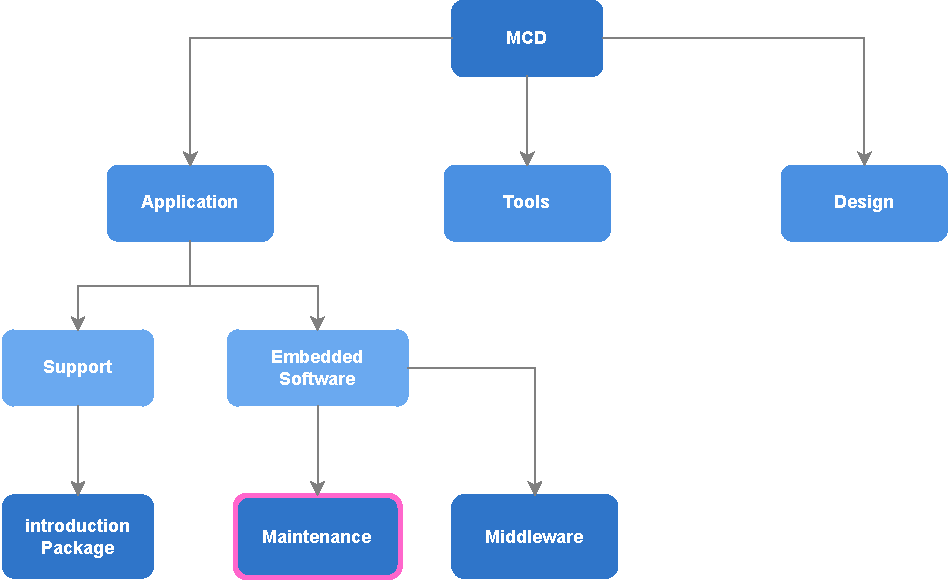
\includegraphics[width=0.7\textwidth]{Figures/chapter1/st-site-organization.pdf}
\caption{Organisational structure of the Microcontroller Division (MCD) at ST Tunis.
The Maintenance team (highlighted) is the host team of this project.}
\label{fig:st-site-org}
\end{figure}

This project was carried out in the \textbf{Technical Marketing and Application Support}
team under MCD. This team includes two sub-teams:

\begin{itemize}
\item \textbf{The GitHub team}: supports customers via GitHub, publishes updates of HAL
drivers, and maintains example projects to facilitate application development based on
STM32 microcontrollers.
\item \textbf{The Maintenance and Validation team}: ensures customer satisfaction through
bug maintenance and functional validation of manufactured microcontrollers and their
associated HAL versions. This team represents the junction linking software and hardware
design processes to implementation and industrialisation.
\end{itemize}

\section{Project presentation}
\label{sec:project-presentation}

\subsection{Project framework}

As part of our training in Computer Engineering at the Faculty of Sciences of Tunis (FST),
University of Tunis El~Manar (UTM), we conclude our education with an end-of-studies
project (PFE). In this context, our project --- entitled \emph{STM32Cube Competitor
Benchmark} --- took place within STMicroelectronics Tunis over a period of six months
(February--September 2026).

\subsection{Project context}
\label{sec:project-context}

The embedded microcontroller market is highly competitive. When an engineer evaluates an MCU
for a new design, the choice between STMicroelectronics and competing vendors (GigaDevice
GD32, NXP, Texas Instruments, Renesas) often depends on measurable differences: firmware
footprint, execution speed, middleware maturity, and development-tool productivity. The
technical marketing team at ST needs objective, reproducible data that quantifies where the
STM32Cube ecosystem outperforms its competitors, where gaps exist, and what concrete
enhancements would close those gaps.

At the start of this project, no systematic benchmarking methodology existed within the
team. Cross-vendor comparisons were ad-hoc, performed manually on a case-by-case basis,
and difficult to reproduce or communicate convincingly to stakeholders.

\subsection{Problematic}
\label{sec:problematic}

Producing actionable competitive intelligence for the marketing team requires answering
precise questions: for a given software stack (e.g.\ USB device, FreeRTOS integration),
running identical scenarios on ST and on a competitor, how do the two platforms compare in
flash and RAM footprint, execution performance, and middleware completeness? And where ST
lags, what specific enhancements --- at the HAL, middleware, or configuration level ---
would close the gap?

Answering these questions rigorously raises several challenges:

\begin{enumerate}
\item \textbf{Scenario design}: each benchmark must exercise the same functionality on both
platforms under identical, well-defined conditions so that the comparison is fair and the
results are meaningful.
\item \textbf{Porting fidelity}: reproducing an STM32 reference scenario on a competitor
requires preserving exact runtime semantics --- task structure, timing, synchronisation,
reporting format --- to avoid comparing apples to oranges.
\item \textbf{Result extraction and interpretation}: raw numbers (kilobytes, cycles,
milliseconds) must be attributed to comparable architectural layers and interpreted in
terms of engineering trade-offs, not merely listed.
\item \textbf{Scale and reproducibility}: the team needs to cover multiple vendors and
multiple stacks with consistent methodology, so that results are comparable across
campaigns and over time.
\end{enumerate}

\subsection{Proposed solution}
\label{sec:proposed-solution}

Our solution is a structured benchmarking methodology centred on three deliverables:

\begin{enumerate}
\item \textbf{Benchmark scenarios}: for each software stack under evaluation (USB device
stack, FreeRTOS, etc.), we design a set of concrete, reproducible scenarios that both the
STM32 reference and the competing platform must run identically. Each scenario exercises a
specific aspect of the stack (e.g.\ HID, CDC, and MSC for USB device).
\item \textbf{Comparative results and interpretation}: for each scenario, we extract
per-layer footprint figures, execution metrics, and qualitative observations, then
interpret them to show where ST is stronger, where the competitor leads, and why.
\item \textbf{Enhancement proposals}: where the data reveals a gap unfavourable to ST, we
identify the root cause and propose targeted improvements --- whether at the HAL driver
level, in middleware configuration, or in linker/startup overhead.
\end{enumerate}

To support this workflow at scale and ensure reproducibility, we developed two supportive
tools in parallel:

\begin{itemize}
\item \textbf{MCU Workflow Studio} --- a cross-vendor firmware footprint analysis
application that automates linker-map comparison, layer classification, and result export
(detailed in Chapter~2).
\item \textbf{MCU Benchmark Copilot Agent} --- a custom AI agent system that accelerates
benchmark creation, porting, and debugging while enforcing fairness and semantic
equivalence (detailed in Chapter~3).
\end{itemize}

These tools are parallel engineering contributions that enhance the benchmarking effort;
they are not the benchmarks themselves. The core deliverable remains the benchmark results
and the enhancement proposals they yield.

\subsection{Mission and objectives}
\label{sec:objectives}

The mission of this internship is to provide the STMicroelectronics technical marketing
team with rigorous, reproducible, and interpretable competitive benchmark data. Specifically,
the project aims to:

\begin{enumerate}
\item Design benchmark scenarios for selected software stacks, ensuring fairness and
semantic equivalence between ST and each competitor.
\item Execute the benchmarks on representative hardware, extracting flash/RAM footprint,
execution performance, and qualitative observations per scenario.
\item Compare and interpret the results layer by layer, highlighting where ST excels and
where gaps exist.
\item Formulate concrete enhancement proposals for STM32Cube where the data reveals room
for improvement.
\item Develop supportive tools (footprint analyser, benchmark agent) to make the
methodology reproducible and scalable beyond this project.
\end{enumerate}

\section{Theoretical foundations}
\label{sec:theory}

This section presents the background concepts essential for understanding the technical
aspects of the project: the STM32 microcontroller ecosystem, firmware memory footprint, and
the linker-map artefact that our tools consume.

\subsection{STM32 microcontrollers}
\label{sec:stm32-overview}

\subsubsection{Overview}

A microcontroller unit (MCU) is an integrated circuit that combines a processor core,
memory (flash and RAM), and peripherals on a single chip. It is designed for embedded
applications where cost, power, and real-time determinism are critical constraints.

\subsubsection{The STM32 family}

The STM32 family from STMicroelectronics is a series of 32-bit microcontrollers based on
ARM Cortex-M processor cores, produced since 2007~\cite{stm32-family}. The family spans
four macro groups --- high-performance, mainstream, ultra-low-power, and wireless --- with
more than ten product sub-families. Each sub-family targets a different balance of
processing power, memory, peripherals, and energy efficiency.

The ARM Cortex-M profile is optimised for embedded applications requiring low cost and low
power consumption~\cite{arm-cortexm}. Cortex-M cores range from the M0 (simplest, lowest
gate count) to the M7 and M33 (highest performance, with DSP and optional floating-point
units). STM32 devices span this entire range.

\subsubsection{The STM32Cube ecosystem}

STMicroelectronics provides a comprehensive software ecosystem around its STM32 hardware
~\cite{stm32cube-ecosystem}:

\begin{itemize}
\item \textbf{STM32CubeMX}: a graphical configuration tool that generates initialisation
code for peripherals, clocks, and middleware.
\item \textbf{STM32CubeIDE}: an integrated development environment based on Eclipse, with
build, flash, and debug support.
\item \textbf{STM32Cube firmware packages}: per-family packages containing the HAL and
low-level (LL) drivers, middleware (FreeRTOS, USB, FatFS, LwIP, mbedTLS), board support
packages (BSP), and example projects.
\item \textbf{STM32CubeProgrammer}: a flashing and option-byte configuration utility.
\item \textbf{STM32CubeMonitor}: a real-time variable monitoring tool.
\end{itemize}

It is this ecosystem --- not merely the silicon --- that we benchmark against competitors.
When we compare ``ST versus GD32,'' we compare the full software stack each vendor provides
for a given use case, because that is what an engineer evaluates when choosing a platform.

\subsection{Firmware memory footprint}
\label{sec:footprint-theory}

The memory footprint of firmware is the amount of non-volatile (flash) and volatile (RAM)
memory it occupies once compiled and linked. Flash stores read-only code and constant data;
RAM stores read-write data (global and static variables, plus stack and heap at run time).

Footprint is a first-class metric in MCU benchmarking for several reasons. Flash and RAM
are fixed, on-chip resources; every kilobyte consumed by the vendor's software stack is a
kilobyte unavailable for application logic. A smaller footprint enables the use of a
cheaper device with less memory, directly affecting bill-of-materials cost. It also leaves
headroom for future features and reduces power consumption in flash-retention scenarios.

Comparing footprint across vendors is non-trivial because each vendor structures, names,
and layers its code differently. The same peripheral initialisation appears as
\texttt{HAL\_GPIO\_Init} on STM32, \texttt{GPIO\_PinInit} on NXP, and \texttt{R\_IOPORT\_Open}
on Renesas. A fair comparison must map these correspondences and attribute costs to
comparable architectural layers (application, middleware, low-level driver, system runtime).

\subsection{Linker maps}
\label{sec:linker-maps}

The linker map is a text file produced by the linker at the end of the build process. For
the IAR Embedded Workbench for ARM (EWARM) toolchain~\cite{iar-ewarm}, this file lists
every module and function that was linked into the final image, together with its code size
(read-only), constant-data size (read-only), and variable-data size (read-write). It also
records the memory sections, placement addresses, and total resource usage.

The linker map is the single input to our footprint analysis tool. By parsing it, we can
reconstruct the complete static memory budget of a firmware build without instrumenting or
executing the code. This makes the measurement perfectly reproducible: the same source code,
compiler version, and optimisation level always produce the same map.

\section{Work methodology}
\label{sec:methodology}

We adopted a ``divide and conquer'' approach~\cite{divide-conquer}, decomposing the project
into well-scoped tasks with clear deliverables and deadlines:

\begin{enumerate}
\item \textbf{Task~1 --- Literature and ecosystem study}: research the STM32Cube
ecosystem, competing vendor ecosystems (GD32, NXP, TI, Renesas), linker-map formats,
and existing benchmarking practices.
\item \textbf{Task~2 --- Benchmark scenario design}: define the software stacks to
benchmark, select representative boards for ST and each competitor, and design fair,
reproducible scenarios with identical observable behaviour on both sides.
\item \textbf{Task~3 --- Benchmark execution and porting}: build and validate each
scenario on the STM32 reference, port it to the competitor platform preserving semantic
equivalence, compile both under IAR EWARM, and extract results.
\item \textbf{Task~4 --- Result comparison and interpretation}: compare per-layer
footprint, execution metrics, and qualitative observations; identify where ST excels and
where gaps exist; formulate enhancement proposals.
\item \textbf{Task~5 --- Supportive tool development} (parallel): design and implement
MCU Workflow Studio (footprint analysis) and the MCU Benchmark Copilot Agent (benchmark
creation and porting assistant) to make the methodology scalable and reproducible.
\item \textbf{Task~6 --- Documentation and report}: document the methodology, tools, and
results in this report.
\end{enumerate}

% TODO: Add Gantt chart figure once the timeline image is available
% \begin{figure}[H]
% \centering
% \includegraphics[width=\textwidth]{Figures/gantt.pdf}
% \caption{Gantt chart of the project schedule (February--September 2026).}
% \label{fig:gantt}
% \end{figure}

\section*{Conclusion}

In this chapter, we introduced STMicroelectronics and its Tunis site, presented the
competitive context that motivates cross-vendor benchmarking, and defined the core mission:
design benchmark scenarios, execute them on ST and competitor platforms, compare and
interpret the results for the marketing team, and propose targeted enhancements where ST can
improve. Two supportive tools developed in parallel make this methodology reproducible and
scalable. The theoretical foundations --- the STM32Cube ecosystem, firmware footprint, and
linker maps --- provide the vocabulary for the chapters that follow. Chapter~2 and
Chapter~3 present the supportive tools, while subsequent chapters present the benchmark
results themselves.


\chapter{A Cross-Vendor Firmware Footprint Analysis Tool}
\label{chap:footprint-tool}

\section*{Introduction}

Comparing STMicroelectronics against a competing vendor is, at bottom, a measurement
problem: the same workload is built for both platforms and the resulting binaries are
weighed against one another. One of the most revealing measurements is the
\emph{memory footprint} of the firmware --- how much flash and RAM a given software stack
consumes once compiled and linked. Footprint is easy to define but tedious to compare
fairly across ecosystems, because two vendors rarely name, split, or organise their code
the same way. To make this comparison reproducible rather than artisanal, we designed and
built a dedicated desktop and command-line application, \emph{MCU Workflow Studio}, that
ingests the linker output of two builds and produces a layer-aware, explainable footprint
comparison between an STM32 reference and a competitor.

This chapter documents that tool as an engineering contribution in its own right. We first
state the problem it solves and the requirements we set for it, then describe its
architecture and its end-to-end pipeline, the implementation choices behind its
deterministic core and its optional language-model assistance, how it plugs into the wider
benchmarking effort, and finally its concrete value and its current limitations.

\section{The cross-vendor footprint problem}
\label{sec:tool-problem}

The flash and RAM budget of a microcontroller unit (MCU) is a hard constraint. Every
kilobyte of code competes with application logic for a fixed amount of on-chip memory, and
it ripples into device cost, power, and the headroom left for future features. When we
benchmark a software stack --- a Universal Serial Bus (USB) device stack, a real-time
operating system integration, and so on --- the footprint each vendor charges for the same
functionality is
therefore a first-class metric.

Measuring it fairly is the difficult part. A modern build links application code against a
vendor software development kit (SDK) whose drivers, middleware, and startup code are structured to that
vendor's own conventions. The same peripheral initialisation appears as
\texttt{HAL\_GPIO\_Init} on STM32, as \texttt{GPIO\_PinInit} on one competitor, and as
\texttt{fsl\_gpio} routines on another; equivalent middleware sits in different modules, and
the boundary between "driver" and "system runtime" is drawn differently in each toolchain.
Doing the comparison by hand means reading two linker maps side by side, guessing which
symbol on one side corresponds to which on the other, and summing kilobytes into comparable
buckets --- slow, subjective, and impossible to reproduce exactly two weeks later.

We set the tool a small number of firm requirements. It had to be \textbf{deterministic and
reproducible}, so that the same inputs always yield the same verdict. It had to be
\textbf{layer-aware}, grouping symbols into architectural layers so that "ST spends more in
the hardware abstraction layer (HAL)" can be stated precisely. Its symbol matching had to be
\textbf{explainable}, attaching a confidence and a reason to every correspondence rather
than hiding behind a black box. It had to treat \textbf{ST as the reference} against which
each competitor is measured. And it had to \textbf{export} its results in formats the rest
of the report can consume directly.

\section{Design and architecture}
\label{sec:tool-architecture}

The tool is organised as a thin set of user interfaces wrapped around a deterministic
comparison core, with an SQLite-backed knowledge base alongside and an optional,
off-by-default block of language-model assistance. Figure~\ref{fig:tool-architecture}
shows the arrangement. Data flows top to bottom: a build's linker map enters through the
ingestion layer, is classified into architectural layers, is compared symbol by symbol in
the core, and leaves as a set of exported artefacts.

\begin{figure}[H]
\centering

\includegraphics[width=\textwidth]{Figures/footprint-tool/architecture.pdf}
\caption{Layered architecture of the footprint-analysis tool. A deterministic comparison
core (ingestion, classification, mapping, comparison, export) is wrapped by the user
interfaces and backed by an SQLite knowledge base; an optional, off-by-default
AI-assistance column refines the mapping without ever sitting on the critical path.}
\label{fig:tool-architecture}
\end{figure}

\begin{figure}[H]
\centering

\includegraphics[width=\textwidth]{Figures/footprint-tool/use-case.pdf}
\caption{UML use-case diagram of MCU Workflow Studio~v0.2.0. Five actors interact with
twenty use cases grouped by concern: the benchmark engineer drives the core analysis, the
technical reviewer validates low-confidence mappings, the CI/CD pipeline runs scripted
headless benchmarks, the LLM service (optional, dashed) enriches the mapping, and the
equivalence miner maintains the cross-vendor knowledge base.}
\label{fig:tool-use-case}
\end{figure}

\begin{figure}[H]
\centering

\includegraphics[width=\textwidth]{Figures/footprint-tool/sequence.pdf}
\caption{UML sequence diagram of a complete footprint benchmark run. The workflow service
orchestrates twelve steps: parsing both linker maps, classifying symbols into layers,
querying the equivalence database, scoring candidates with twelve weighted signals,
computing per-layer deltas, evaluating firmware quality metrics, and emitting the run
manifest alongside all export artefacts.}
\label{fig:tool-sequence}
\end{figure}

Two interfaces sit on top of the same engine: a desktop graphical user interface (GUI) built with PySide6
(the Qt binding for Python)~\cite{pyside6}, which provides over fourteen analysis tabs ---
including interactive charts, a mapping mind-map visualisation panel, a review queue, and a
project-scoped chat assistant --- and a command-line interface for scripted and reproducible
runs. Both call
into a single \emph{workflow service} that owns the data models and drives every stage.
Persistence is handled by SQLite~\cite{sqlite}: a vendor registry of aliases and naming
prefixes, a knowledge store of confirmed correspondences, an optional feedback store, and a
history of past runs. The block of language-model features on the right is genuinely
optional --- the deterministic path produces a complete result without it --- and we return
to it in Section~\ref{sec:tool-ai}. Table~\ref{tab:tool-io} lists what the tool consumes
and what it produces.

\begin{table}[H]
\centering
\caption{Principal inputs and outputs of the tool.}
\label{tab:tool-io}
\begin{tabularx}{\textwidth}{l X}
\toprule
\textbf{Inputs} & \textbf{Description} \\
\midrule
IAR EWARM \texttt{.map} ($\times 2$) & Linker maps of the source (STM32) and target (competitor) builds; the only required inputs. \\
Prior workbook (\texttt{.xlsx}) & Optional earlier results re-used as a baseline. \\
Vendor identifiers & Source and target vendor names (default \texttt{stm32}/\texttt{nxp}) that select the alias and prefix tables. \\
\midrule
\textbf{Outputs} & \textbf{Description} \\
\midrule
\texttt{benchmark\_results.xlsx} & Per-layer and global flash/RAM comparison with a verdict. \\
Scoped CSV/JSON/XLSX & Filtered exports for downstream processing. \\
Review queue (JSON/CSV) & Low-confidence mappings prioritised for manual confirmation. \\
Mapping diagnostics (JSON) & Per-pair signal breakdown and acceptance decisions. \\
GUI payload (JSON) & Pre-rendered data for the desktop interface. \\
PDF report (optional) & Eight-page narrative summary with charts, quality grade, and enhancement roadmap. \\
Run manifest (JSON) & Tool version, input checksums, equivalence DB hash, and deterministic mode for reproducibility. \\
\bottomrule
\end{tabularx}
\end{table}

\section{The benchmarking pipeline}
\label{sec:tool-pipeline}

A benchmark run is a fixed sequence of stages, sketched in
Figure~\ref{fig:tool-pipeline}. The solid path is purely deterministic; the dashed stages
are the optional language-model steps, which are disabled by default and can be switched on
without changing anything else. After validating its inputs, the tool parses both linker
maps into a common in-memory model --- build metadata, an overall footprint, and the list
of modules and functions with their code and data sizes. Each symbol is then classified
into an architectural layer, and the vendor knowledge (aliases, prefixes, prior matches) is
prepared.

The heart of the run is the mapping stage, where each STM32 symbol is matched to its
closest competitor counterpart by combining several similarity signals into a single,
explainable score. The accepted matches are then aggregated: the tool computes the flash
and RAM totals per layer and globally for both sides, compares them, and emits a verdict
together with recommendations and a root-cause breakdown of where the difference comes
from. Finally it persists the quality of the pair and composes its exports; the optional
advisor, PDF report, and run-history entry are produced only if requested.

\begin{figure}[H]
\centering
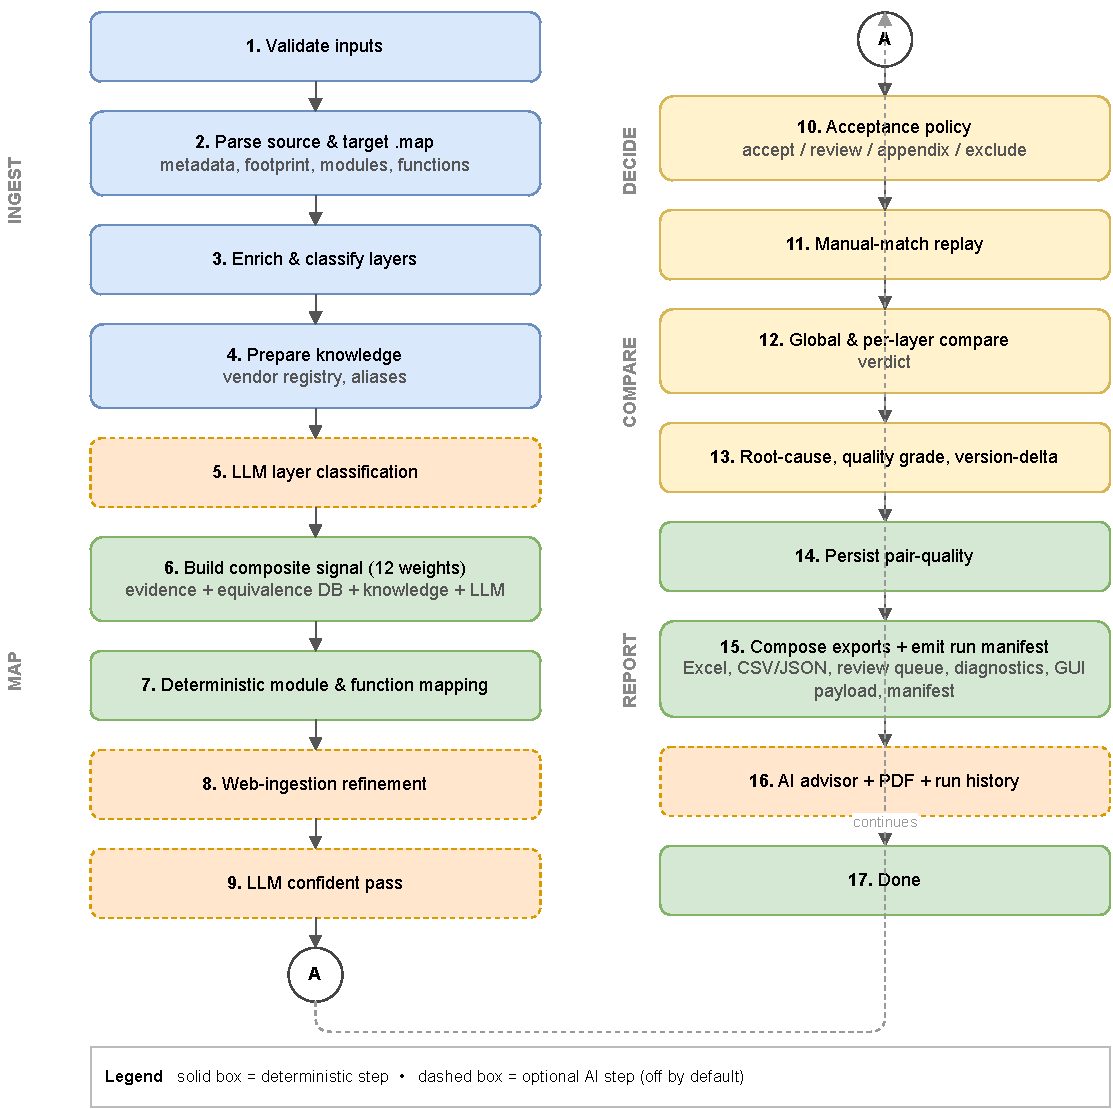
\includegraphics[width=0.9\textwidth]{Figures/footprint-tool/pipeline.pdf}
\caption{End-to-end benchmark pipeline, from linker-map ingestion to report generation.
Dashed stages are optional AI-assisted steps that are disabled by default; the solid
deterministic path runs end to end on its own.}
\label{fig:tool-pipeline}
\end{figure}

A second, lighter mode produces a single-map footprint summary --- validate, parse, classify,
and write a footprint workbook --- which is useful when only one build is available or to
sanity-check a map before a full comparison.

\section{Implementation}
\label{sec:tool-implementation}

The tool is written entirely in Python ($\geq$~3.11)~\cite{python}, with a small,
deliberately conventional dependency set summarised in Table~\ref{tab:tool-stack}. We
favoured the standard library wherever it was sufficient: all persistence uses the built-in
SQLite engine~\cite{sqlite}, and every network call to a language model goes through the
standard \texttt{urllib} module rather than a vendor SDK, which keeps the executable small
and the dependency surface auditable. The whole application can be packaged into a
stand-alone Windows executable with PyInstaller~\cite{pyinstaller}.

\begin{table}[H]
\centering
\caption{Implementation stack and the role of each external dependency.}
\label{tab:tool-stack}
\begin{tabularx}{\textwidth}{l l X}
\toprule
\textbf{Concern} & \textbf{Technology} & \textbf{Role in the tool} \\
\midrule
Language & Python $\geq$ 3.11 \cite{python} & Entire code base (version 0.2.0). \\
Desktop GUI & PySide6 / Qt \cite{pyside6} & 14+ tab windows, mind-map panel, chat assistant. \\
Tabular export & pandas \cite{pandas} & Scoped CSV/JSON/Excel export. \\
Excel I/O & openpyxl \cite{openpyxl} & Reads prior workbooks, writes results. \\
Charts \& PDF & matplotlib \cite{matplotlib} & Figures in the 8-page PDF report. \\
Persistence & SQLite \cite{sqlite} & Knowledge base, equivalence store, run history. \\
Packaging & PyInstaller \cite{pyinstaller} & Stand-alone Windows executable. \\
\bottomrule
\end{tabularx}
\end{table}

\subsection{Parsing linker maps and classifying layers}
\label{sec:tool-parsing}

The single required input is the linker map emitted by the IAR Embedded Workbench for ARM
(EWARM) toolchain~\cite{iar-ewarm}. The parser reads this map and reconstructs, for
each module and function, the read-only code and data it contributes and the read-write data
it reserves. From these we derive the two footprint figures the benchmark cares about: flash
occupancy as the sum of read-only code and read-only data, and RAM occupancy as the
read-write data. This is a \emph{static} measurement taken from the linked image; it captures
what the firmware costs to store, not its dynamic stack or heap behaviour at run time, and we
are careful to present it as such.

Each symbol is then assigned to one of four architectural layers --- application, middleware,
low-level driver, or system runtime --- by a deterministic classifier driven by module names,
known vendor prefixes, and section attributes. This layering is what lets the final report say
not merely that one firmware is larger, but \emph{where} it is larger, which is far more useful
when the goal is to understand a vendor's engineering trade-offs.
Figure~\ref{fig:tool-layer-classification} details the decision flow.

\begin{figure}[H]
\centering
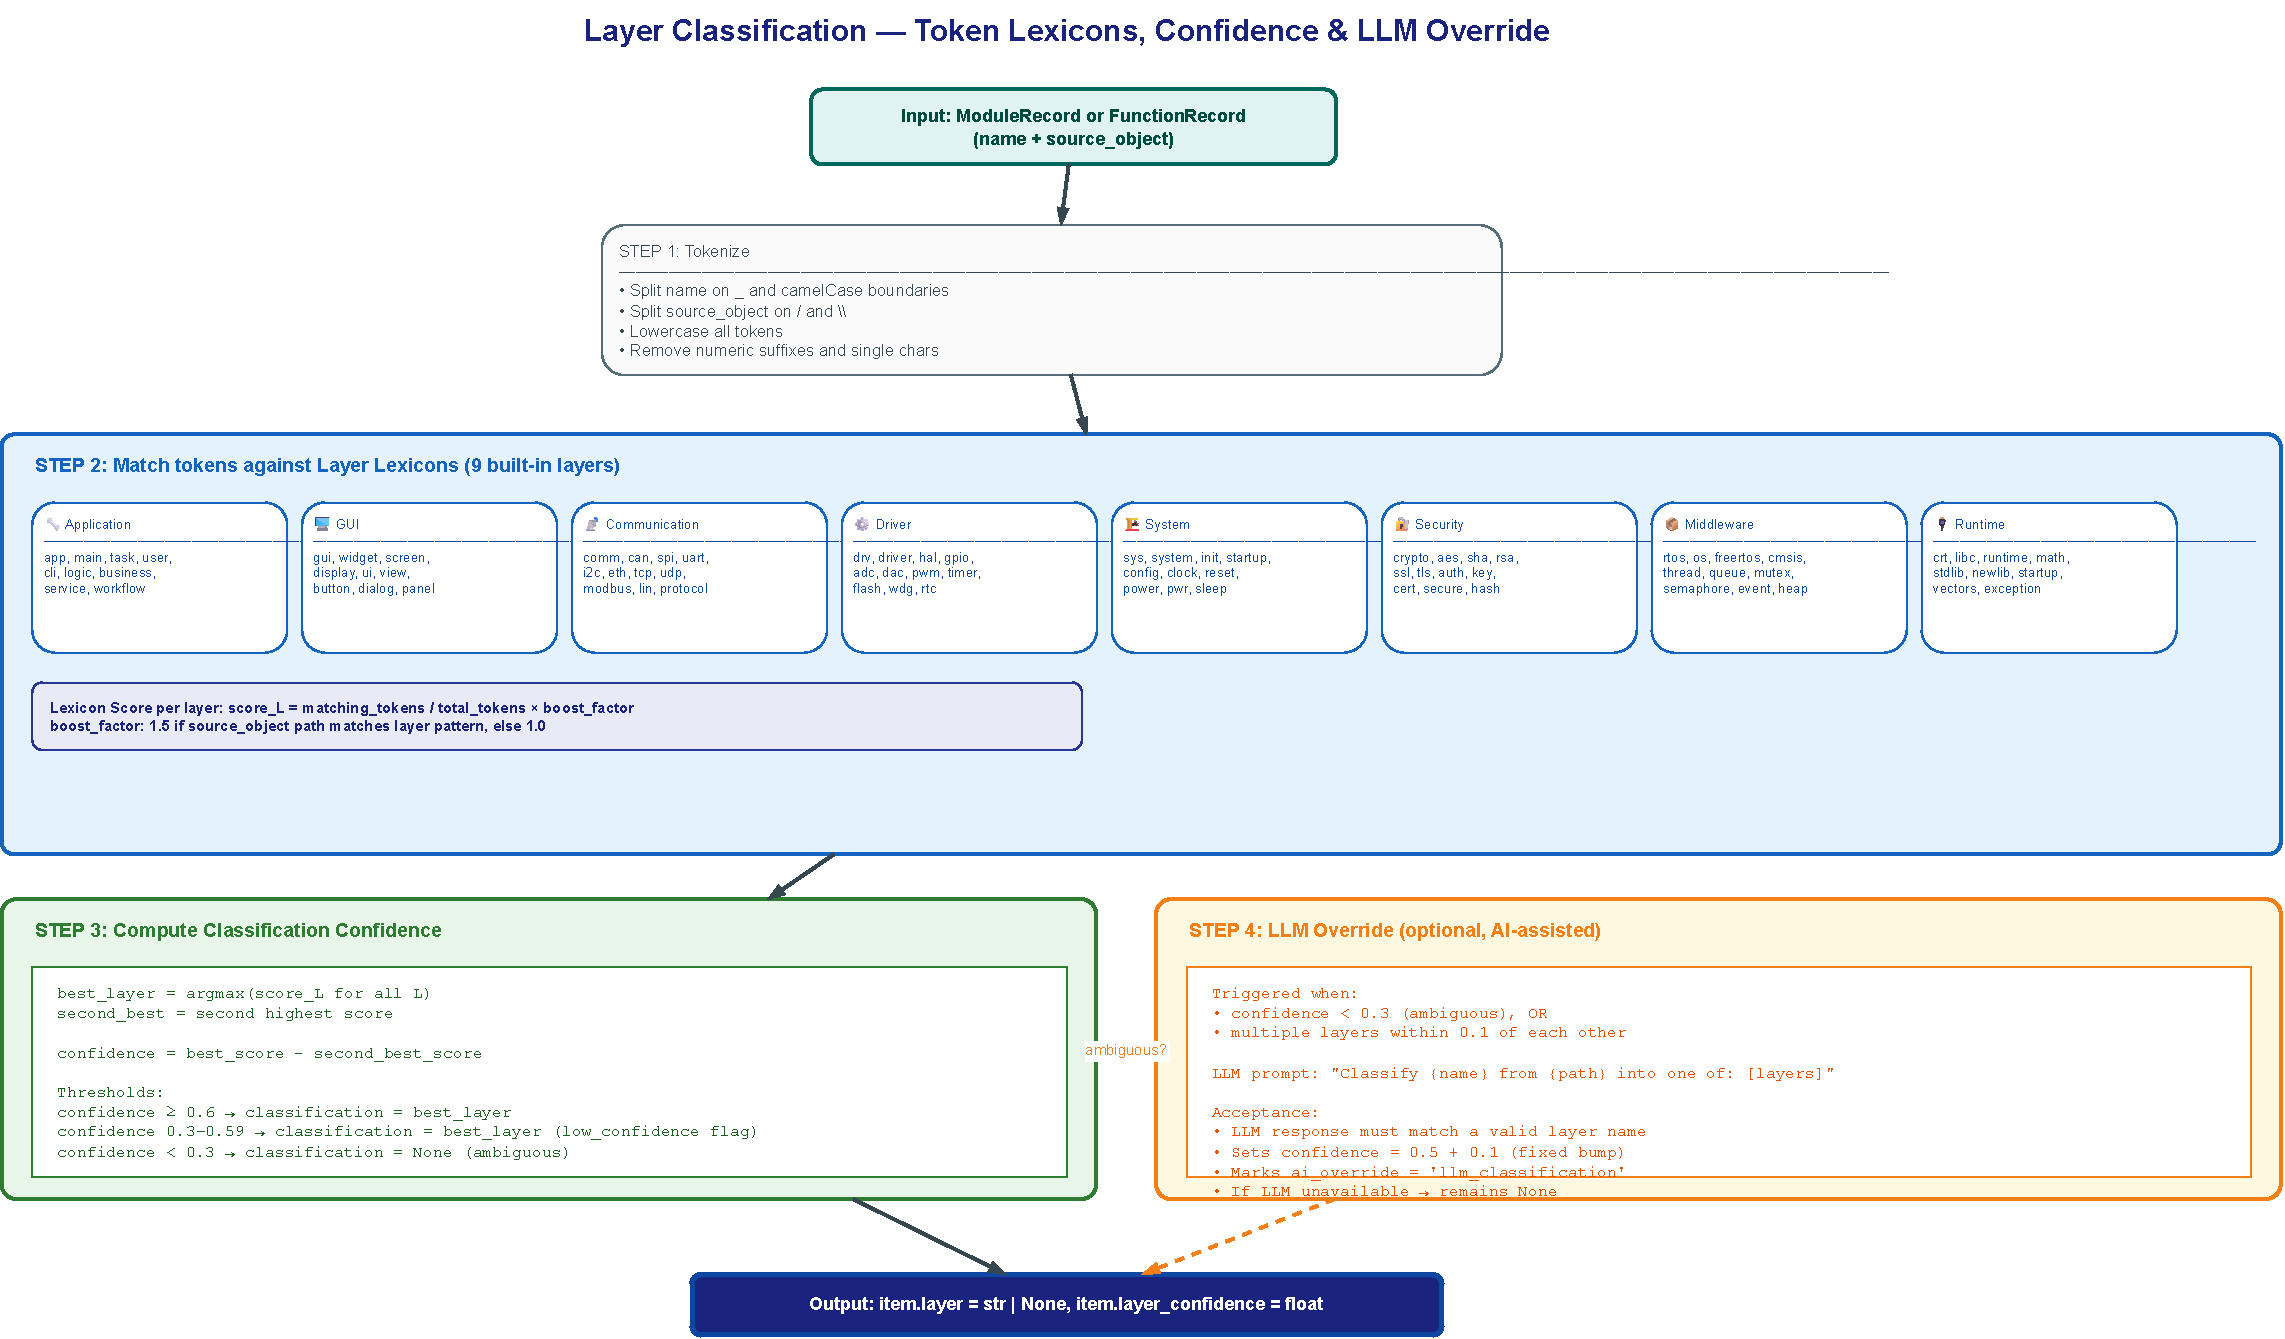
\includegraphics[width=\textwidth]{Figures/footprint-tool/layer-classification.pdf}
\caption{Layer-classification decision flow. Each symbol's tokens are matched against
priority-ordered lexicons (system, middleware, low-level, application); the first match
determines the layer with an associated confidence.}
\label{fig:tool-layer-classification}
\end{figure}

\subsection{The multi-signal mapping engine}
\label{sec:tool-mapping}

Matching ST symbols to their competitor counterparts is the part that, done manually, costs the
most time and is the least repeatable, so it received the most care. Rather than rely on name
similarity alone --- which fails precisely when two vendors name the same function differently
--- the engine scores each candidate pair by combining twelve weighted signals into a single,
explainable confidence value. Role similarity and alias similarity carry the most weight
(0.18 each), followed by name similarity and operation similarity (0.12 each), external
references and signature cues (0.10 each), footprint proximity (0.08), object similarity
(0.06), context cues (0.04), and three knowledge-base priors (history, board-pair,
scenario --- contributing the remaining 0.02). The weights sum to exactly~1.0.
Figure~\ref{fig:tool-weights} shows the relative weights, and
Figure~\ref{fig:tool-scoring-signals} expands the computation and penalty mechanics of each
signal.

\begin{figure}[H]
\centering
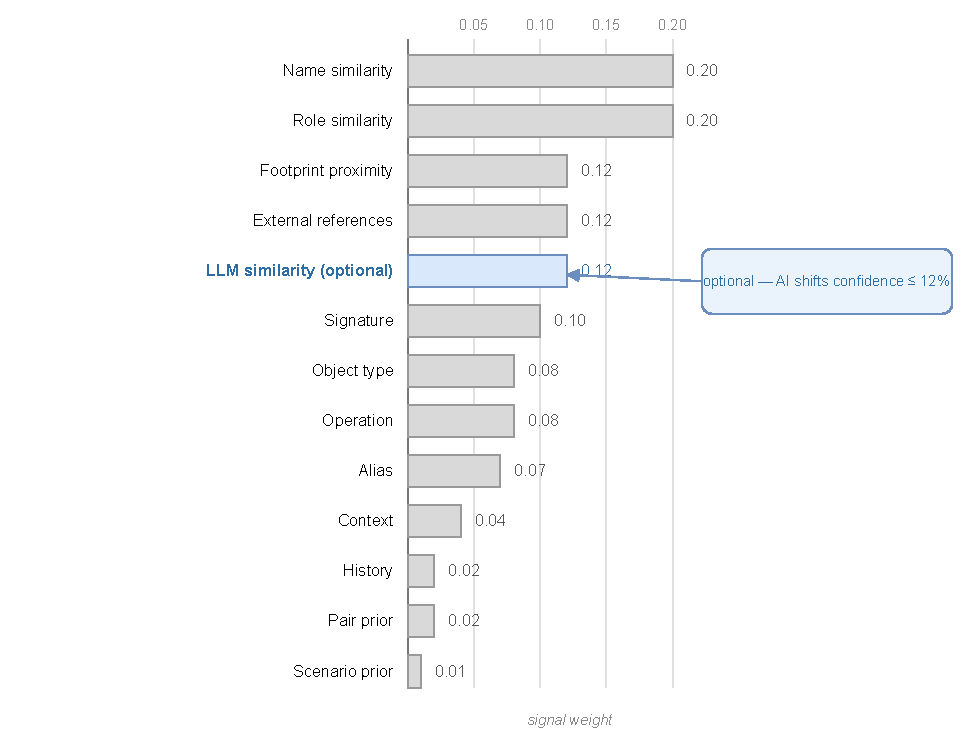
\includegraphics[width=0.88\textwidth]{Figures/footprint-tool/weights.pdf}
\caption{Relative weights of the signals combined by the deterministic mapping scorer. Name
and role similarity dominate; the optional LLM-similarity signal (highlighted) is capped so
that AI assistance can shift a candidate's confidence by at most twelve percent.}
\label{fig:tool-weights}
\end{figure}

\begin{figure}[H]
\centering
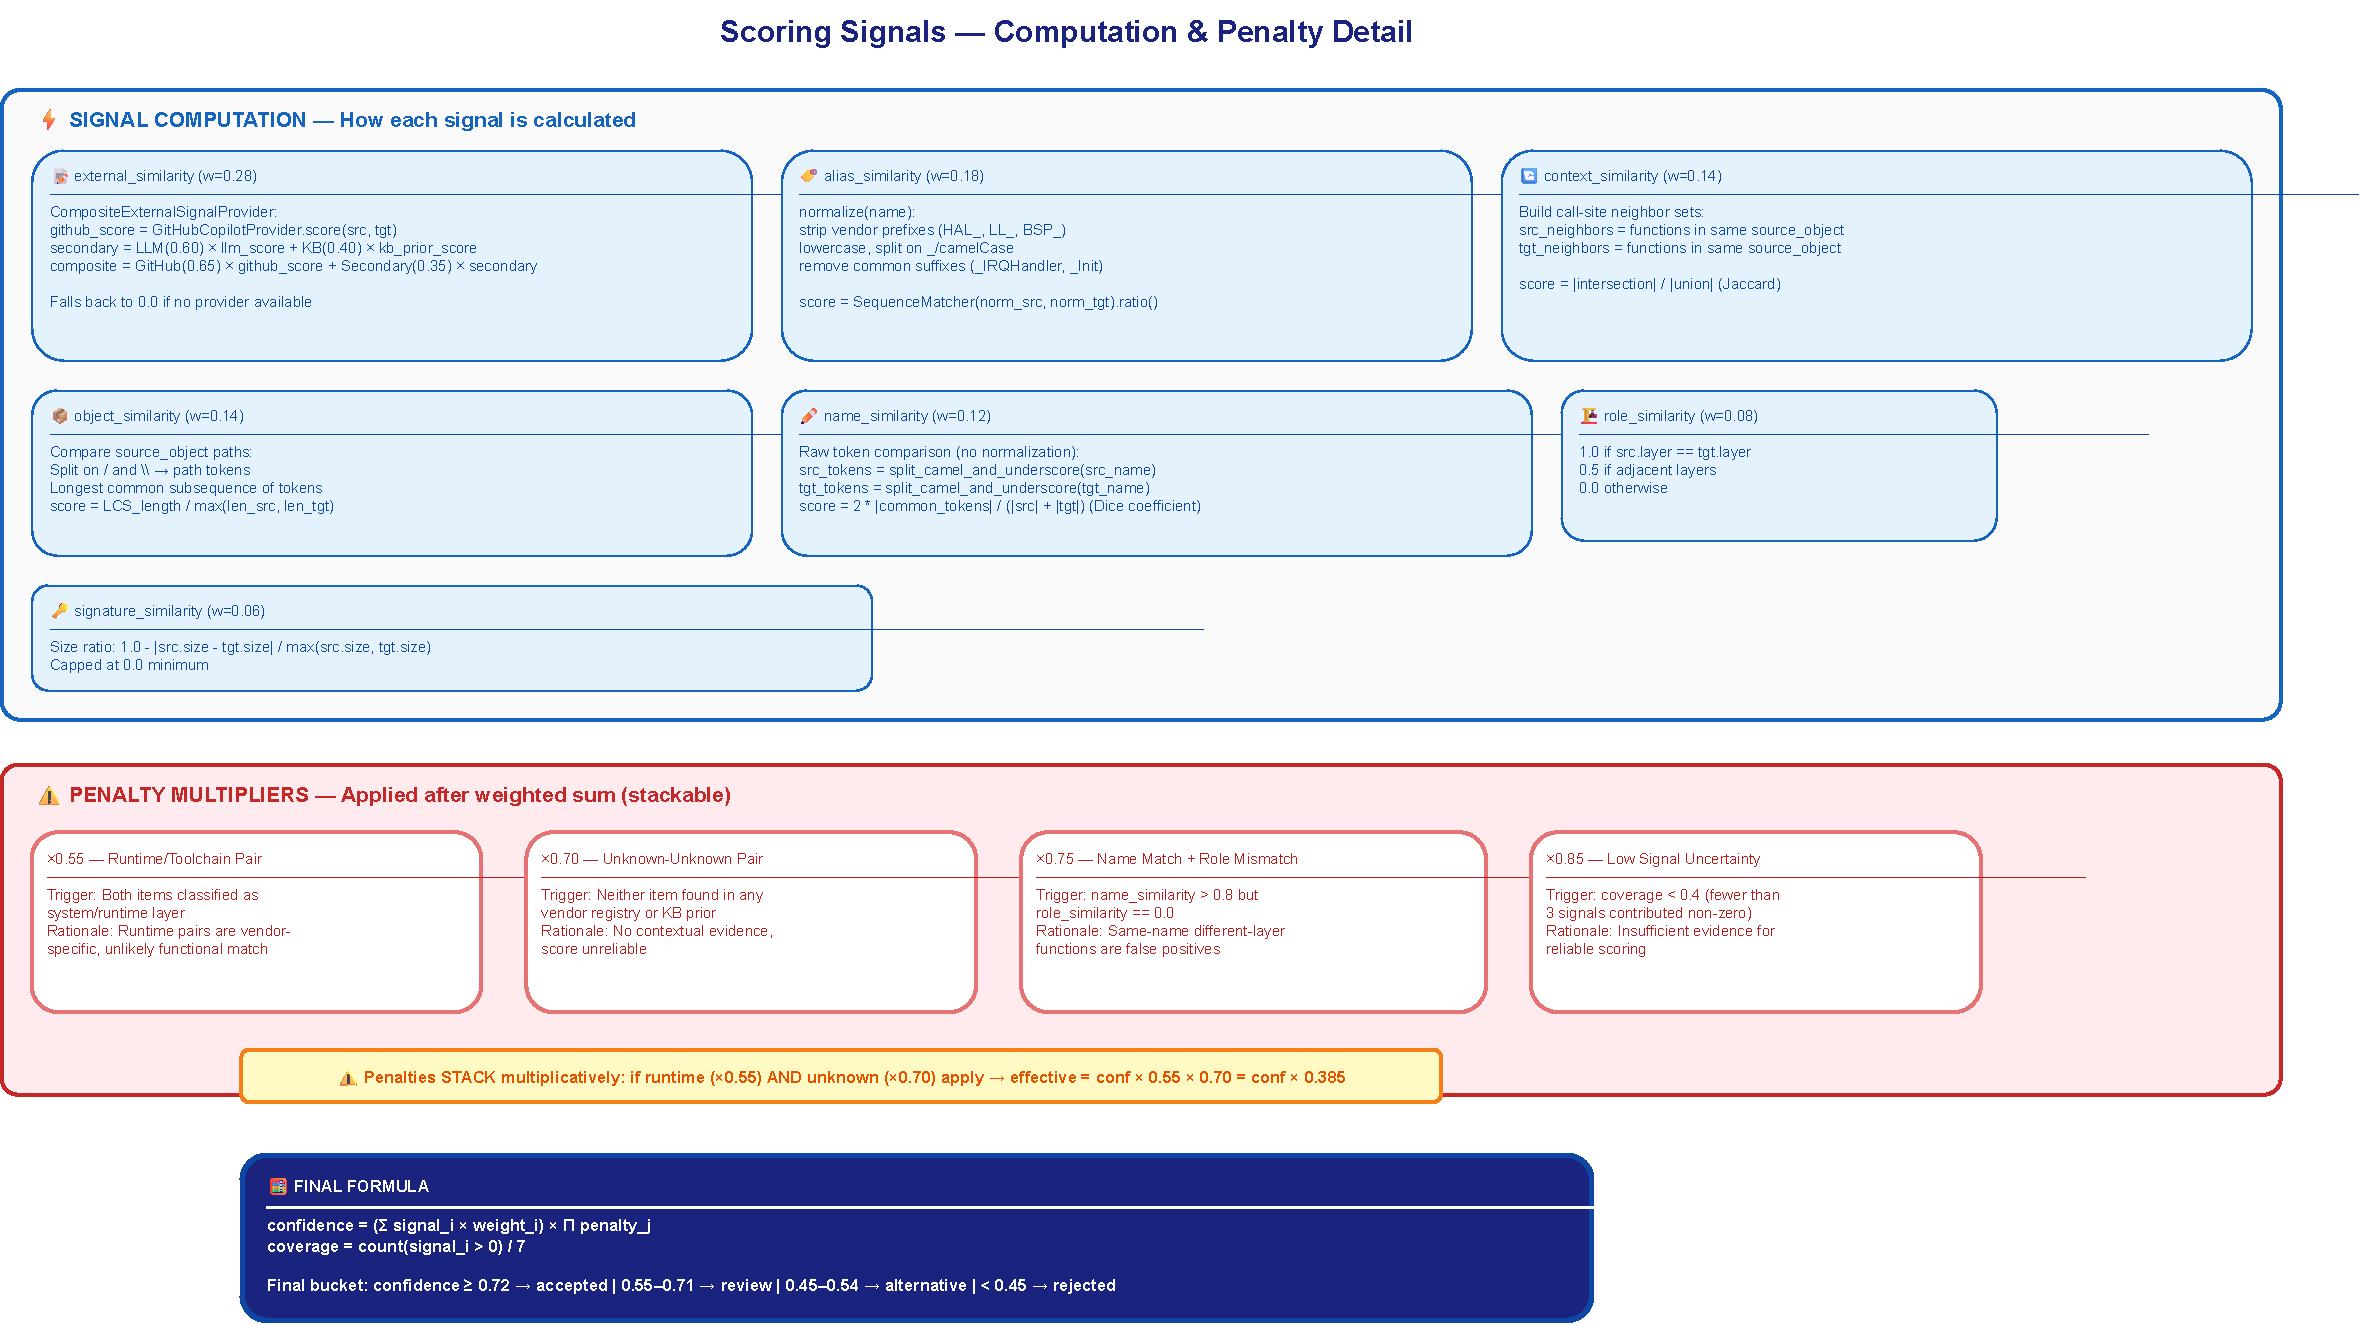
\includegraphics[width=\textwidth]{Figures/footprint-tool/scoring-signals.pdf}
\caption{Detailed signal computation and penalty system. Seven evidence signals are computed
for each candidate pair; penalties for size mismatch and layer conflict reduce the composite
score before the acceptance threshold is applied.}
\label{fig:tool-scoring-signals}
\end{figure}

The resulting confidence drives a transparent acceptance policy. A correspondence is accepted
automatically once its confidence reaches $0.72$, queued for manual review above $0.55$, kept
as a weaker alternative above $0.45$, and an unmatched symbol is retained on its own only above
$0.80$. The engine also records the cardinality of each match --- one-to-one, one-to-many, or
many-to-one --- which matters because vendors routinely split or merge functionality
differently, and a one-to-many match is itself a finding about how the two stacks are
structured. Every decision, with its per-signal breakdown, is written to the mapping
diagnostics so that a reviewer can see exactly why two symbols were paired.
Figure~\ref{fig:tool-candidate-ranking} illustrates the complete flow from candidate
generation through pruning, scoring, and threshold-based bucketing.

\begin{figure}[H]
\centering
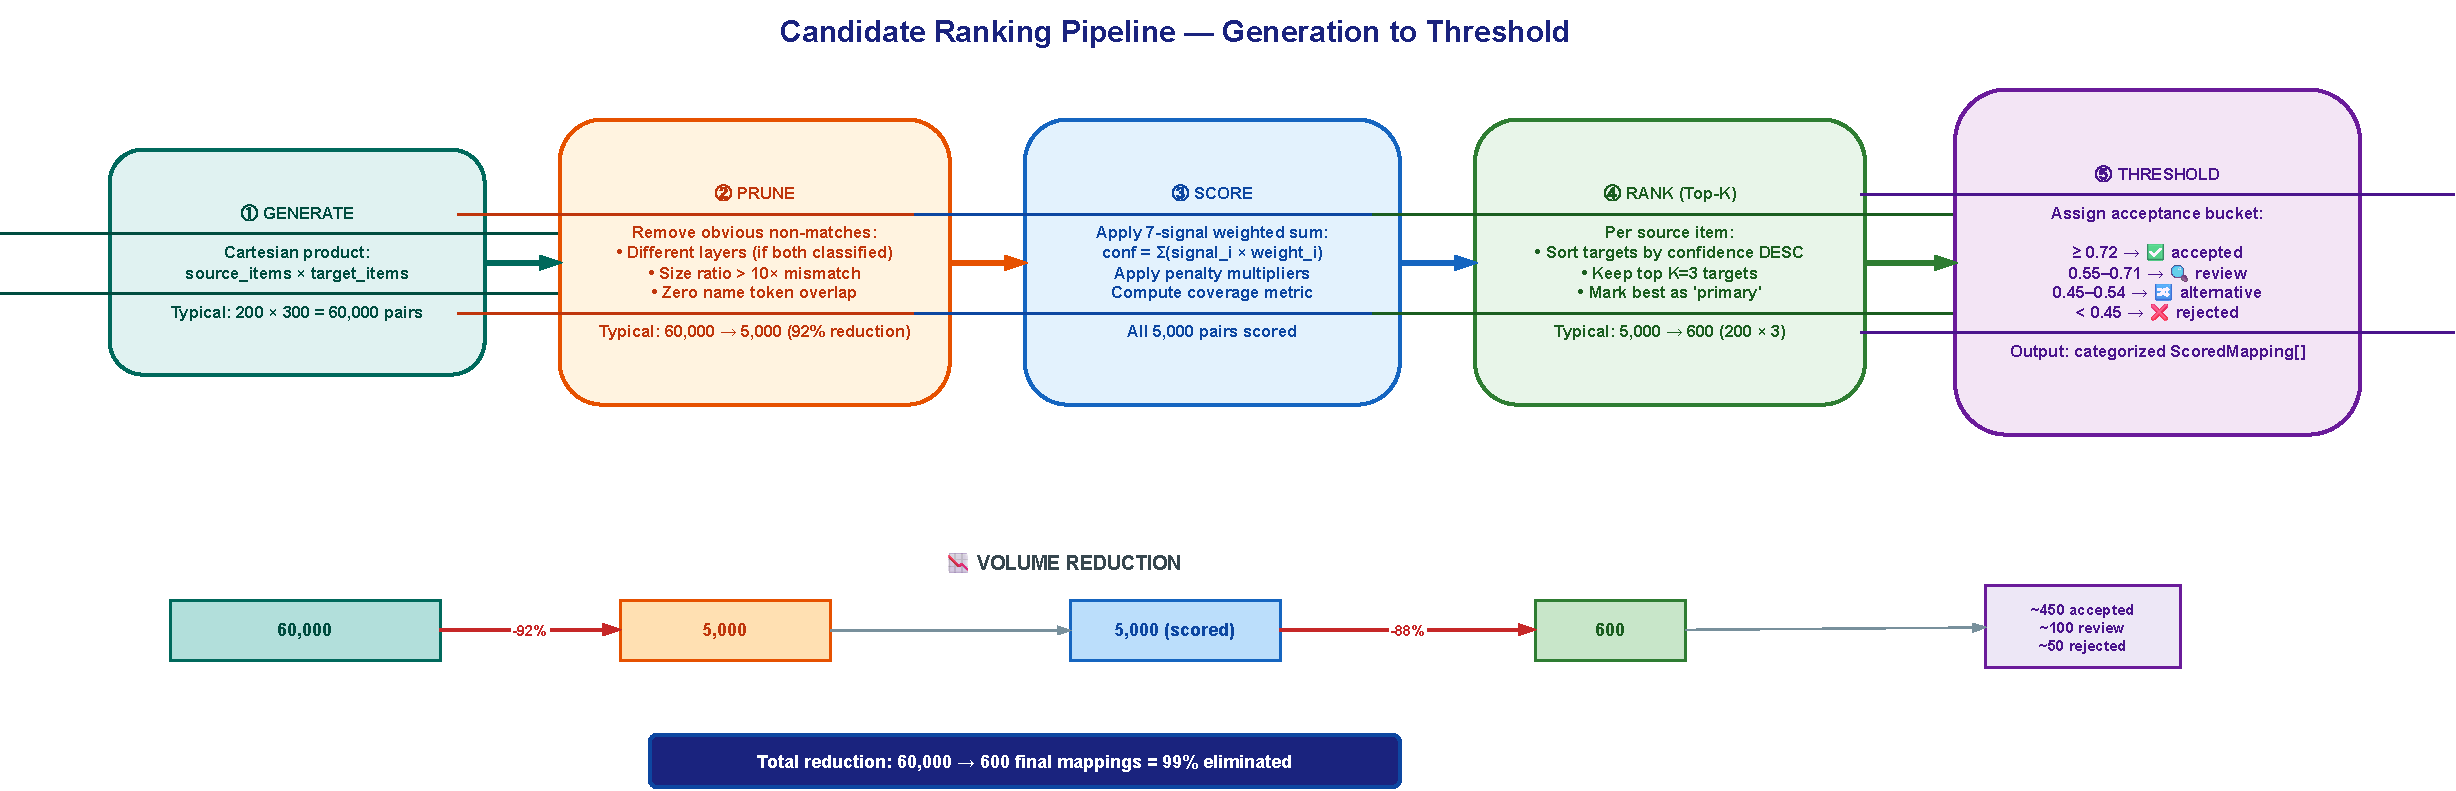
\includegraphics[width=\textwidth]{Figures/footprint-tool/candidate-ranking.pdf}
\caption{Candidate generation, ranking, and threshold flow. The Cartesian product of source
and target items is pruned by fast rejection filters, scored on all signals, and bucketed
into accepted, review, alternative, and unmatched categories by confidence thresholds.}
\label{fig:tool-candidate-ranking}
\end{figure}

\subsection{Optional AI assistance}
\label{sec:tool-ai}

The tool is best described as a deterministic core with \emph{optional} language-model
assistance, not as an "AI tool" in the sense of one that cannot work without a model. Every
language-model feature is opt-in and disabled by default, and the engine produces a complete,
reproducible result with all of them switched off. When they are enabled, they act in three
bounded ways. First, a large language model (LLM) can supply one additional
similarity signal during mapping; as Figure~\ref{fig:tool-weights} makes explicit, that signal
is weighted and capped so it can move a candidate's confidence by at most twelve percent, and
the run stays within a fixed call budget. Second, a "confident pass" may confirm or reject
borderline matches, and an advisor may suggest where STM32 firmware could be tightened.
Third, the desktop interface offers a chat assistant for exploring a comparison in natural
language.

These features can be served by several interchangeable back-ends, listed in
Table~\ref{tab:tool-ai}, selected automatically in a fixed order or pinned explicitly. They
range from a hosted GitHub Copilot endpoint~\cite{github-copilot} to a fully offline Ollama
server~\cite{ollama}, so the assistance can run without any data leaving the machine. If a
back-end is unavailable or returns something unusable, the tool degrades gracefully to its
deterministic output rather than failing. Figure~\ref{fig:tool-ai-integration} shows the
provider abstraction and the auto-detection fallback chain.

\begin{figure}[H]
\centering
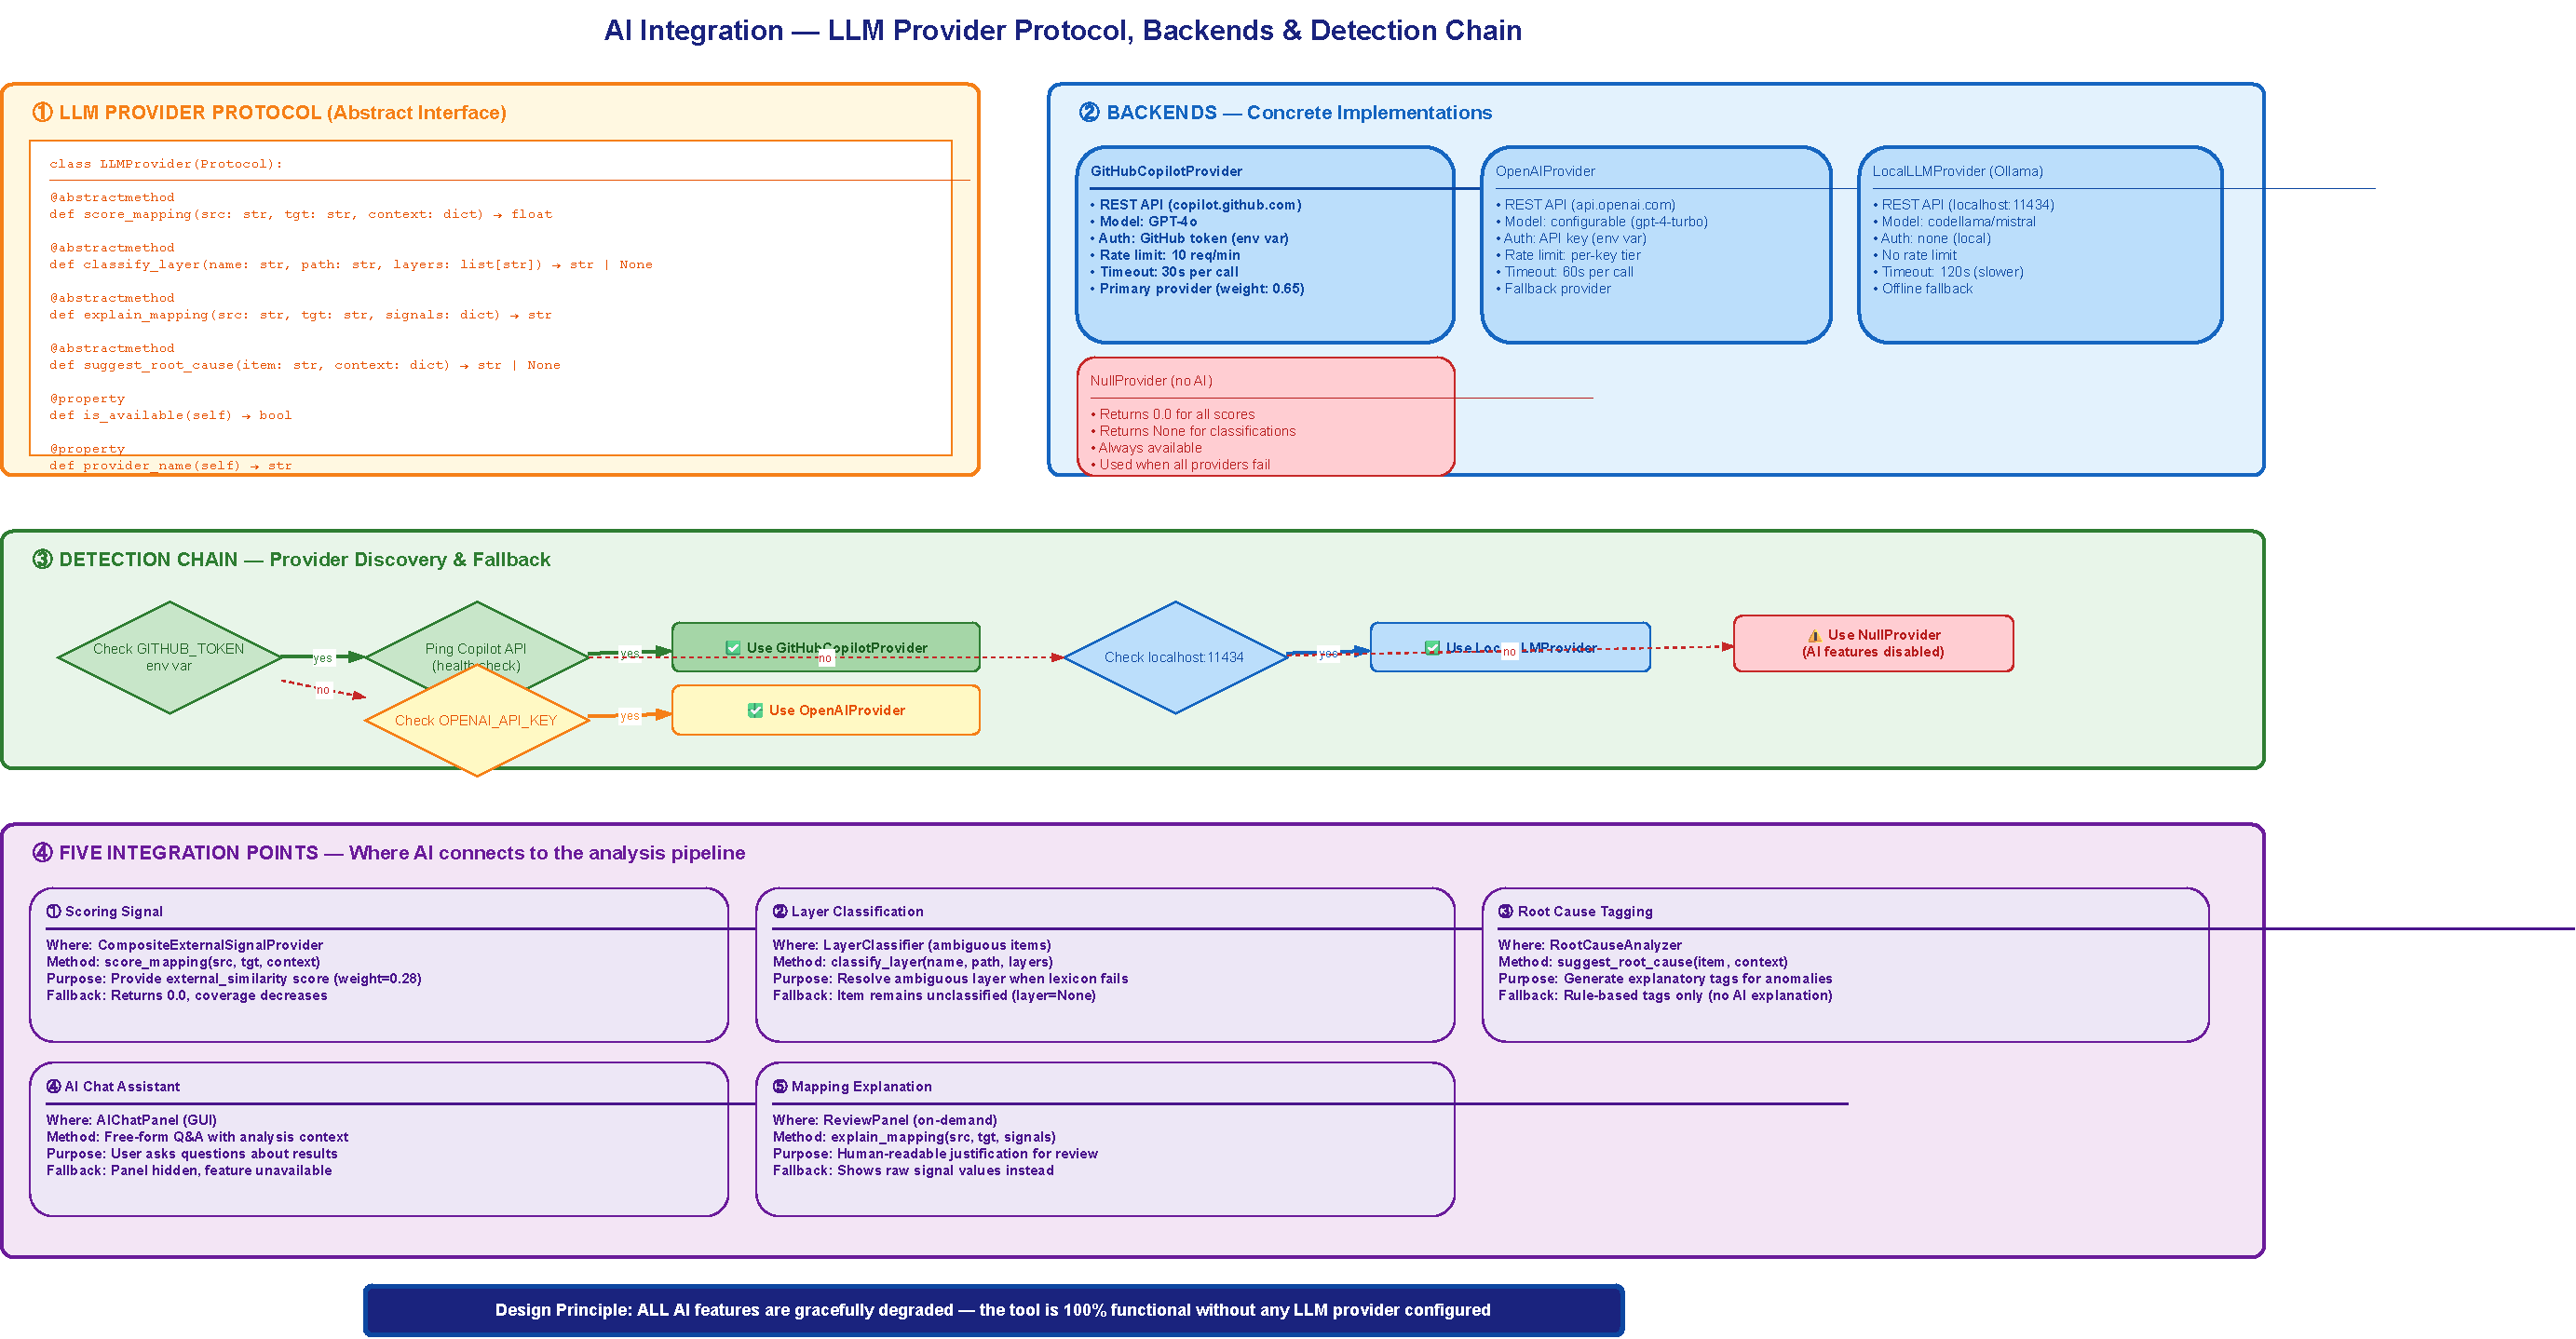
\includegraphics[width=\textwidth]{Figures/footprint-tool/ai-integration.pdf}
\caption{AI integration flow. A common protocol abstracts all back-ends; an auto-detection
chain probes them in priority order (Copilot, OpenAI, Ollama) and falls back gracefully to
purely deterministic operation if none is available.}
\label{fig:tool-ai-integration}
\end{figure}

\begin{table}[H]
\centering
\caption{Optional language-model back-ends. All are disabled by default; the tool runs fully
without them.}
\label{tab:tool-ai}
\begin{tabularx}{\textwidth}{l l X}
\toprule
\textbf{Back-end} & \textbf{Default model} & \textbf{Selection / requirement} \\
\midrule
GitHub Copilot \cite{github-copilot} & Claude (Anthropic) \cite{anthropic} & OAuth device flow; first in the auto-detect order. \\
OpenAI \cite{openai-api} & GPT-4o & \texttt{OPENAI\_API\_KEY} environment variable. \\
Ollama \cite{ollama} & Llama 3.1 (8B) & Local server; fully offline. \\
GitHub Models \cite{github-models} & gpt-4.1-mini & Default for the narrative assistant. \\
\bottomrule
\end{tabularx}
\end{table}

\subsection{Persistence and learning}
\label{sec:tool-persistence}

All state lives in local SQLite databases: the vendor registry, the store of confirmed
correspondences, a cache of assistant responses, and a history of runs. A manual confirmation
made during review can be replayed on later runs, so the tool improves as it is used on a given
vendor pair. We treat this learning, together with the web-ingestion and run-history features,
as useful but experimental, and none of it is on the critical path of a comparison.

\subsection{Cross-vendor equivalence database}
\label{sec:tool-equivalence}

A critical addition to the scoring engine is the \emph{cross-vendor equivalence database},
which encodes deterministic knowledge about which modules and functions serve the same
peripheral function across vendor SDKs. When two symbols are confirmed equivalents by this
database, their confidence is boosted to the high-confidence threshold regardless of naming
differences.

The database covers twenty-five peripheral groups (GPIO, UART, SPI, I\textsuperscript{2}C,
Timer, Clock, Power, DMA, USB Device, USB Host, Flash, ADC, DAC, CAN, Ethernet, RTC,
Watchdog, CRC, RNG, I\textsuperscript{2}S, Pin Mux, Interrupt, Cortex core, BSP/Board,
System Init, Startup, and PWM) with token-pattern entries for six vendors: STM32, NXP,
Renesas, TI, GigaDevice, and Infineon. It also encodes sixteen action-verb equivalence
classes (init/deinit, start/stop, transmit/receive, set/get, reset, callback, register/
unregister, lock/unlock, suspend/resume), so that \texttt{HAL\_GPIO\_Init} and
\texttt{GPIO\_Setup} are recognised as serving the same role.

The database is designed as an offline, provenance-tracked artefact: an equivalence miner
extracts entries from pinned vendor SDK repositories (resolved to a specific commit SHA for
reproducibility), records provenance for every entry, and produces a content-hashed mining
manifest. This ensures that the equivalence knowledge used in any given run is auditable
and frozen --- it cannot drift silently between executions.

\subsection{Source-code signal provider}
\label{sec:tool-source-code}

When both source and target IAR EWARM project directories are available, an optional
source-code signal provider enriches the mapping with three additional signals derived from
the actual C source files: function signature similarity (parameter count and return-type
patterns), call-graph structural similarity (shared callee patterns), and include-graph
co-location (functions in files with similar \texttt{\#include} dependencies). This
provider operates as an external-signal plug-in to the scoring engine and is disabled by
default; when enabled, it provides a richer correspondence basis for firmware that is
available locally, without requiring any network access or language model.

\subsection{Firmware quality metrics and grading}
\label{sec:tool-quality}

Beyond comparing two builds, the tool computes firmware quality metrics for the source
(STM32) firmware independently: total flash and RAM, module and function counts, average
and maximum module size, layer-balance score, modularity score, code density, HAL
abstraction ratio, middleware ratio, application ratio, large-module count, dead-weight
estimate, optimisation potential, and an overall quality grade (A through~F). These metrics
appear in the PDF report and help the technical marketing team assess not just how STM32
compares to a competitor, but how well the STM32 firmware itself is structured.

\subsection{Run manifest and reproducibility}
\label{sec:tool-manifest}

Every benchmark run emits a \emph{run manifest} that captures the tool version, the
deterministic mode (strict or assisted), the schema version, input file checksums, and a
hash of the equivalence database state at the time of execution. This manifest allows any
run to be proven reproducible: given the same inputs, configuration, and frozen knowledge
state, the tool must produce byte-for-byte identical logical output. The deterministic
hardening specification formalises this guarantee by requiring stable sort tie-breaks,
rounded floating-point scores, and canonical export ordering across all stages.

\section{Integration into the benchmark workflow}
\label{sec:tool-integration}

The tool occupies a precise place in our method. Once a software stack has been built for an
STM32 board and for the competing vendor's board under identical scenarios, each build's IAR
linker map is fed to the tool as the source and the target. Its per-layer and global footprint
figures, its verdict, and its root-cause breakdown are exactly the numbers the per-vendor
benchmarking chapters of this report quote when they weigh ST's flash and RAM cost against a
competitor's for a given stack. In other words, the footprint comparisons reported later are not
assembled by hand: they are produced, with an auditable trail, by the tool described here, which
is why we document it before presenting any results that depend on it.

\section{Usage and outputs}
\label{sec:tool-usage}

% TODO(screenshot): Replace placeholder with actual GUI screenshot
\begin{figure}[H]
\centering
\fbox{\parbox{0.9\textwidth}{\centering\vspace{4cm}\textbf{[PLACEHOLDER --- GUI screenshot]}\\Capture the MCU Workflow Studio desktop interface showing a completed\\benchmark comparison (main window with charts and layer breakdown).\vspace{4cm}}}
\caption{MCU Workflow Studio desktop interface showing a USB HID footprint comparison between STM32 and a competitor.}
\label{fig:tool-gui}
\end{figure}

A comparison can be driven either from the desktop interface or, for reproducible and scriptable
runs, from the command line. A typical invocation names the two maps and their vendors and points
at an output directory, as in Listing~\ref{lst:tool-cli}.

\lstset{style=mystyle}
\begin{lstlisting}[language=bash, caption={Command-line invocation of a footprint benchmark.}, label={lst:tool-cli}]
mcu-workflow-cli benchmark \
  --source stm32usbhidclassproject.map --source-vendor stm32 \
  --target nxpusbhidclassproject.map   --target-vendor nxp \
  --out results/
\end{lstlisting}

The run leaves behind the artefacts of Table~\ref{tab:tool-io}: a results workbook with the
per-layer and global comparison, scoped CSV/JSON exports, a prioritised review queue of the
matches that warrant a human look, the full mapping diagnostics, and --- on request --- an
eight-page PDF report with an executive summary, source-versus-target charts, an
architecture-and-module breakdown, a gap analysis, and recommendations. The samples we used to
develop and validate the tool are themselves a representative comparison: a USB human interface device (HID)
class project built for an STM32U575 board against the equivalent project built for an NXP
MCXN947 board~\cite{nxp-mcuxpresso}, both compiled with the same IAR toolchain so that only the
vendor software stacks differ.

% TODO(screenshot): Replace placeholder with actual Excel workbook screenshot
\begin{figure}[H]
\centering
\fbox{\parbox{0.9\textwidth}{\centering\vspace{3cm}\textbf{[PLACEHOLDER --- Results workbook screenshot]}\\Capture a screenshot of \texttt{benchmark\_results.xlsx} open in Excel, showing\\the per-layer comparison sheet with ROM/RAM columns.\vspace{3cm}}}
\caption{Sample output: the results workbook showing per-layer and global footprint comparison.}
\label{fig:tool-results-xlsx}
\end{figure}

% TODO(screenshot): Replace placeholder with actual PDF report page
\begin{figure}[H]
\centering
\fbox{\parbox{0.9\textwidth}{\centering\vspace{3cm}\textbf{[PLACEHOLDER --- PDF report screenshot]}\\Capture the first page (executive summary) of the optional PDF report\\generated by the tool, showing the verdict chart.\vspace{3cm}}}
\caption{First page of the optional PDF report: executive summary with source-vs-target charts.}
\label{fig:tool-pdf-report}
\end{figure}

\section{Engineering value and limitations}
\label{sec:tool-value}

The value of the tool is that it turns a slow, subjective, once-off comparison into a fast,
explainable, and repeatable one. A footprint benchmark that previously took an afternoon of
careful map-reading now runs in seconds and produces the same answer every time, with a
documented reason behind every symbol correspondence and a clear attribution of where each
kilobyte of difference originates. The run manifest, the frozen equivalence database, and the
deterministic hardening guarantee that the same inputs always yield the same verdict ---
satisfying the reproducibility requirement of academic evaluation.

The twelve-signal scoring engine, backed by the cross-vendor equivalence database covering
twenty-five peripheral groups and sixteen action-verb classes, achieves high-confidence
mappings across six vendors without relying on language models. The firmware quality metrics
and grading system provide an independent structural assessment of the STM32 firmware, and
the multi-run history tracks how footprint evolves across SDK versions.

We are equally clear about what the tool does not do. It reads IAR EWARM linker maps; builds
produced by other toolchains are out of scope for now, and broadening the parser is the most
obvious avenue for future work. Its footprint figures are static, derived from the linked image
rather than from execution. The quality grades and optimisation-potential estimates that the
report produces are heuristic indications, not measured quantities, and we label them
accordingly wherever they appear. Finally, the language-model features, while useful, are
optional and still maturing; the trustworthy core of the tool is, and is meant to remain, fully
deterministic.

\section*{Conclusion}

We designed and built MCU Workflow Studio to remove the manual bottleneck in cross-vendor
footprint benchmarking and to make its results reproducible and explainable. Its deterministic
core parses two IAR linker maps, classifies every symbol into an architectural layer, maps
STM32 symbols to their competitor counterparts using a twelve-signal scoring engine backed by a
cross-vendor equivalence database, and reports per-layer and global flash and RAM differences
with a clear root cause. The run manifest guarantees reproducibility; the firmware quality
metrics provide an independent structural assessment; and the optional, strictly bounded
language-model assistance enriches the mapping without ever sitting on the critical path. The
chapters that follow rely on this tool for the footprint figures they report, which is why we
have presented it first, as a contribution in its own right.


\chapter{An Autonomous AI Agent for Benchmark Campaigns}
\label{chap:benchmark-agent}

\section*{Introduction}

The previous chapter presented a tool that analyses the \emph{output} of a benchmark ---
two linker maps produced by completed builds. However, producing those builds in the first
place is itself a substantial engineering task. Each new cross-vendor comparison requires
creating a benchmark project for the competitor platform, porting the STM32 reference code
while preserving its exact runtime semantics, configuring the IAR Embedded Workbench for
ARM (EWARM) project correctly, and debugging the inevitable compiler, linker, and runtime
issues that arise when targeting unfamiliar silicon. Done manually, this process is slow,
error-prone, and difficult to keep consistent across many vendor comparisons.

To address this, we designed and built the \emph{MCU Benchmark Copilot Agent} --- a custom
GitHub Copilot agent system that operates inside Visual Studio Code (VS Code) and
\emph{autonomously} drives end-to-end benchmark campaigns: from scenario resolution and
firmware acquisition, through project creation, IAR build automation, evidence-driven
debugging, measurement extraction, and semantic-equivalence verification~\cite{vscode,
github-copilot}. Unlike a passive assistant, the agent executes builds, fetches missing
materials from official vendor sources, applies fixes, and iterates --- asking the user
only before programming physical hardware. Where MCU Workflow Studio analyses what
\emph{exists}, the agent system \emph{creates} what does not yet exist, and it does so
under strict rules that enforce semantic equivalence and benchmark fairness at every step.
The two tools are complementary: the agent produces validated builds, and the studio
analyses their footprint.

This chapter documents the agent as an engineering contribution. We describe the problem it
addresses, its layered architecture (agents, skills, automation tools, configuration
registry), its deterministic campaign workflow, the always-on policies that govern its
behaviour, and its integration with the broader benchmarking effort.

\section{The benchmark engineering problem}
\label{sec:agent-problem}

A single STM32-versus-competitor benchmark involves several non-trivial steps. The STM32
reference project must first be understood in full --- task structure, timing, peripheral
usage, reporting format, and observable behaviour. A corresponding project must then be
created for the target platform, mapping every STM32 hardware abstraction layer (HAL) call
to the competitor's equivalent application programming interface (API) without altering the
benchmark's semantics. The resulting project must be configured for the IAR
toolchain~\cite{iar-ewarm} with the correct device selection, startup file, linker
configuration, include paths, and compiler defines. Once it compiles, runtime issues --- wrong interrupt vectors,
misconfigured clocks, broken universal asynchronous receiver-transmitter (UART) output ---
must be diagnosed from real evidence rather than guesswork. And throughout, the comparison
must remain fair: same optimisation level, same measurement scope, same observable output
format.

Doing this for one vendor pair and one software stack is manageable. Repeating it for
multiple vendors (GigaDevice, NXP, Renesas, Texas Instruments, Infineon, Nordic,
Microchip) across multiple stacks (USB device, FreeRTOS, CoreMark) quickly becomes the
dominant time cost of the benchmarking campaign. Each port also carries a risk of
\emph{semantic drift} --- subtle changes in task priorities, timing, or synchronisation
that invalidate the comparison without being immediately visible.

We needed a system that could enforce the methodology consistently across every port,
refuse to guess when evidence was missing, execute deterministic build and measurement
workflows without manual intervention, and make its reasoning transparent. A
general-purpose large language model (LLM) cannot do this out of the box: it lacks the
domain-specific checklists, the structured routing, the automation tooling, and the policy
of refusing to claim success without hardware evidence. A custom agent system, built on VS
Code's Copilot extensibility framework, gave us the ability to encode our benchmarking
methodology --- and to \emph{execute} it autonomously --- directly within the development
environment~\cite{vscode-agent-mode}.

\section{Architecture}
\label{sec:agent-architecture}

The system is structured as four cooperating layers: specialist \emph{agents} that handle
reasoning and delegation, reusable \emph{skills} that encode methodology as checklists,
\emph{automation tools} (PowerShell and Python scripts) that perform deterministic
operations, and a \emph{configuration registry} (YAML files) that provides ground truth
about boards, MCUs, vendors, toolchains, and measurement profiles. A shared set of
always-on rules governs all layers. All configuration lives in a \texttt{.github/}
directory within the benchmark workspace --- no compiled code, no external server, no
deployment step. The agents run inside VS Code's GitHub Copilot Chat
extension~\cite{github-copilot} and have access to the workspace file system, terminal,
web, and search capabilities.

Figure~\ref{fig:agent-architecture} illustrates the layered arrangement. A user request
enters the coordinator agent, which resolves the scenario, classifies the task, acquires
missing materials, and delegates to the appropriate specialist agent or invokes a skill
workflow. Specialist agents operate in isolated context, use the automation tools for
deterministic operations, and return structured results.

\begin{figure}[H]
\centering
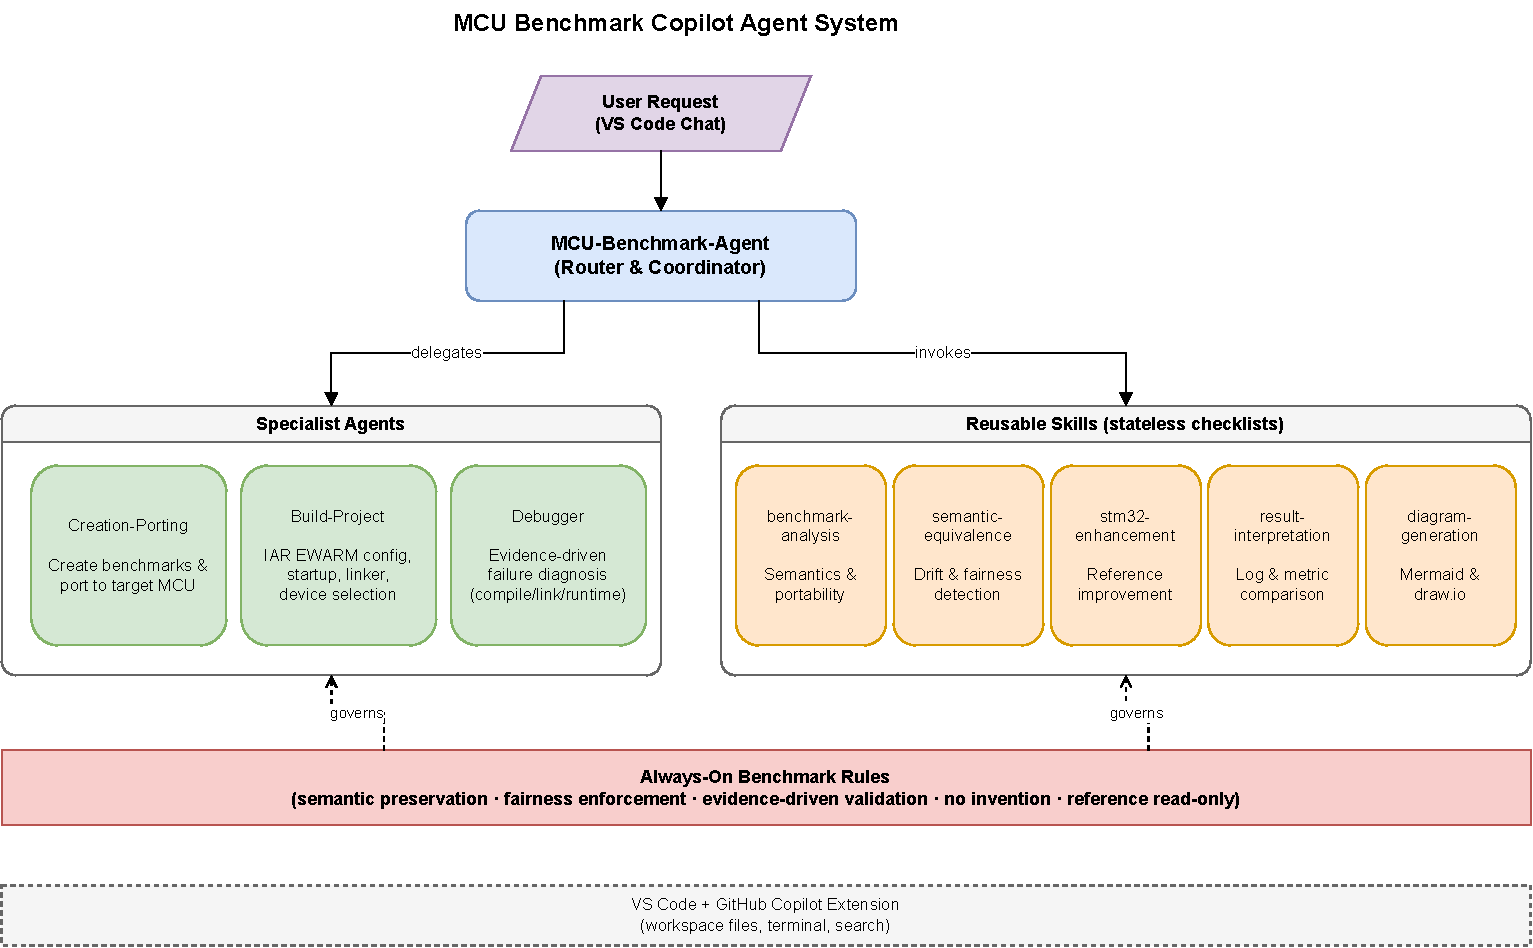
\includegraphics[width=\textwidth]{Figures/benchmark-agent/architecture.pdf}
\caption{Architecture of the MCU Benchmark Copilot Agent system. The coordinator resolves
scenarios and delegates to specialist agents; automation tools handle deterministic
build/measurement operations; all layers operate under the shared always-on benchmark rules
and consult the configuration registry.}
\label{fig:agent-architecture}
\end{figure}

\subsection{The four specialist agents}
\label{sec:agent-specialists}

Each agent has a defined responsibility, a restricted tool set, an autonomy contract, and a
structured output contract. Table~\ref{tab:agent-roles} summarises them.

\begin{table}[H]
\centering
\caption{Specialist agents and their responsibilities.}
\label{tab:agent-roles}
\begin{tabularx}{\textwidth}{l l X}
\toprule
\textbf{Agent} & \textbf{Role} & \textbf{Responsibility} \\
\midrule
MCU-Benchmark-Agent & Autonomous coordinator & Resolves scenarios from partial input, acquires missing materials, orchestrates end-to-end campaigns, delegates to specialists. Full tool access including web and execute. \\
Creation-Porting & Project generation & Creates new benchmark projects from scratch or ports existing benchmarks in any direction (STM32$\to$competitor, competitor$\to$STM32, vendor$\to$vendor, board$\to$board). Acquires firmware autonomously. \\
Build-Project & Build automation & Autonomously executes IAR builds, classifies failures, applies project-level fixes, and rebuilds --- without user intervention for non-hardware tasks. \\
Debugger & Failure diagnosis & Autonomously diagnoses compiler, linker, and runtime failures; extracts measurements from logs and captures; applies minimal fixes and revalidates. \\
\bottomrule
\end{tabularx}
\end{table}

The coordinator's routing decision tree is deterministic: project understanding goes to the
\emph{benchmark-analysis} skill; cross-vendor porting goes to \emph{Creation-Porting};
build execution and configuration go to \emph{Build-Project}; failures accompanied by real
evidence go to \emph{Debugger}; and result interpretation uses the dedicated skill. This
routing prevents a general-purpose model from attempting tasks outside its configured
expertise and ensures each specialist receives only the context it needs.

Figure~\ref{fig:agent-use-case} presents a complete use case diagram of the system,
showing all actors, the twenty internal capabilities, and the hardware approval boundary
that separates autonomous operations from those requiring user confirmation.

\begin{figure}[H]
\centering
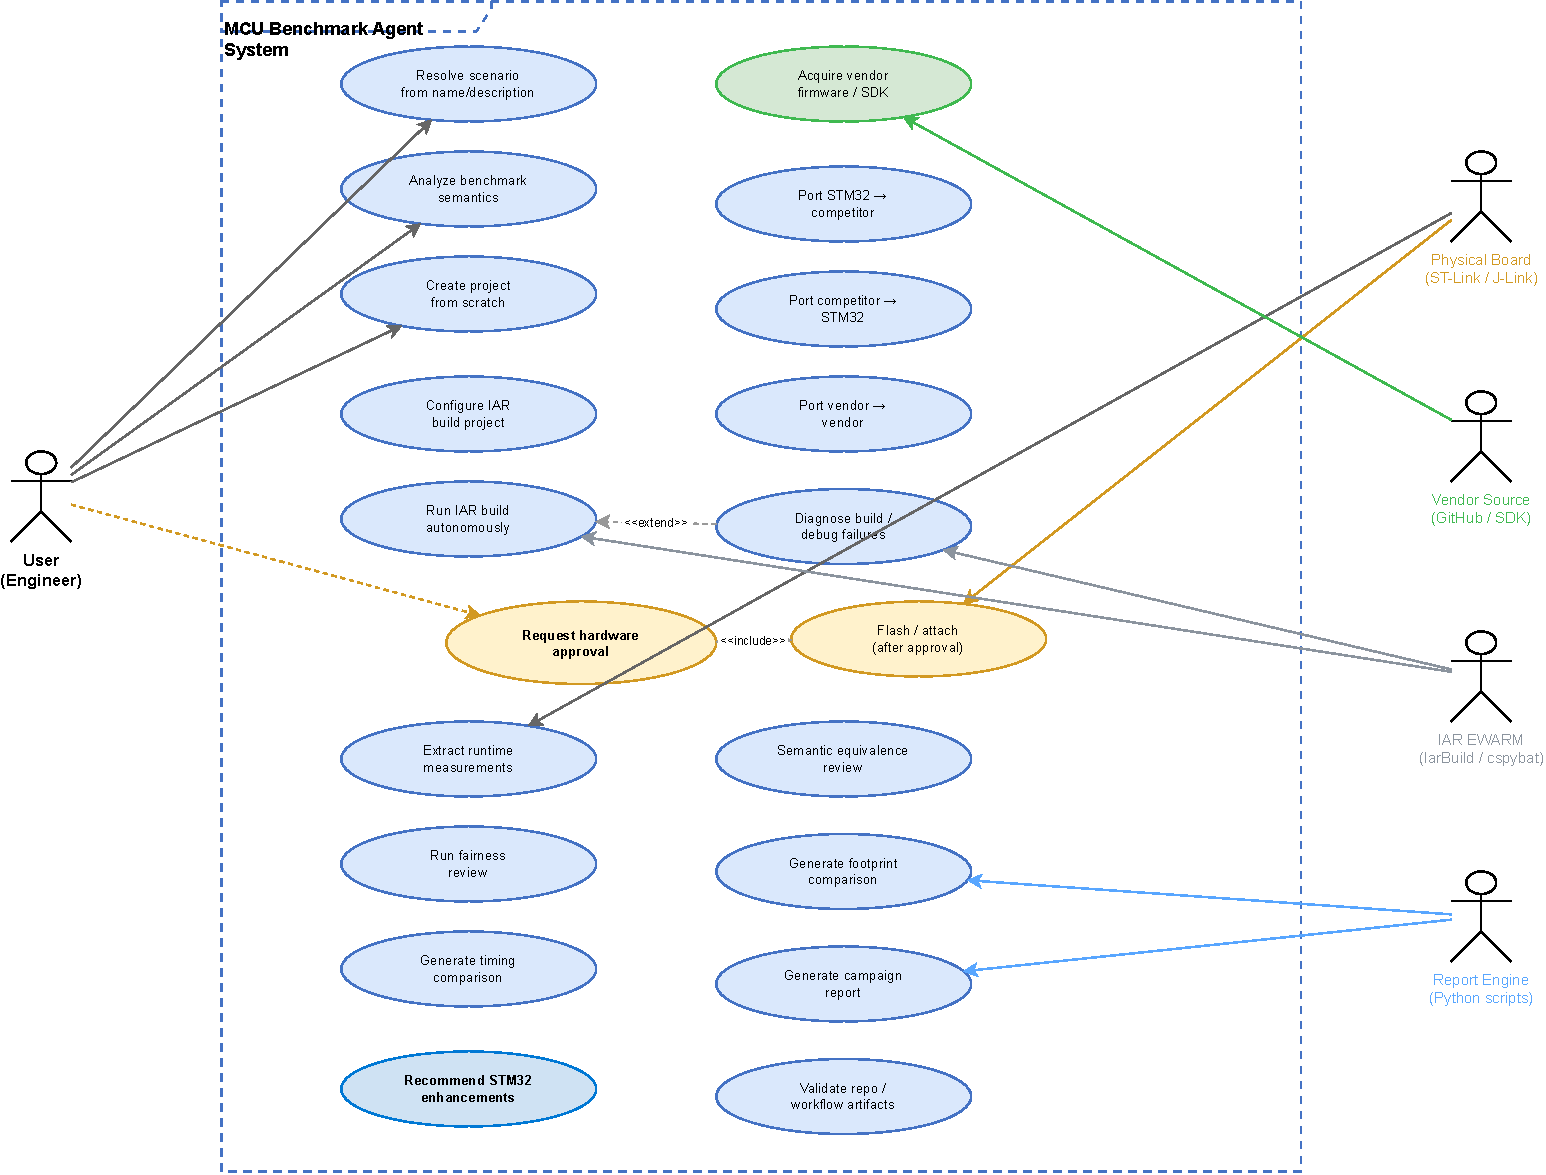
\includegraphics[width=\textwidth]{Figures/benchmark-agent/use-case.pdf}
\caption{UML use case diagram of the MCU Benchmark Copilot Agent system. Blue ellipses
represent autonomous use cases; yellow ellipses require user approval; green indicates
external acquisition. External actors include the user, physical board, vendor source
repositories, IAR EWARM toolchain, and the report engine scripts.}
\label{fig:agent-use-case}
\end{figure}

\subsection{The six reusable skills}
\label{sec:agent-skills}

Skills encode repeatable workflows as structured Markdown checklists. Unlike agents, they
do not receive isolated context or delegated reasoning --- they provide structure, not
autonomy. Table~\ref{tab:agent-skills} lists them.

\begin{table}[H]
\centering
\caption{Reusable skills and their purposes.}
\label{tab:agent-skills}
\begin{tabularx}{\textwidth}{l X l}
\toprule
\textbf{Skill} & \textbf{Purpose} & \textbf{Primary users} \\
\midrule
benchmark-analysis & File classification, semantics extraction, and portability split of an existing project. & Coordinator, Creation-Porting \\
semantic-equivalence & Reference-versus-target behaviour comparison and drift detection. & Coordinator, Creation-Porting \\
iar-template-resolution & Resolve, acquire, and integrate IAR project templates per board type using a deterministic lookup algorithm. & Creation-Porting, Build-Project \\
stm32-enhancement & Gap-driven recommendations for improving STM32 reference portability. & Coordinator \\
result-interpretation & Comparative interpretation of benchmark logs, measurements, and result files. & Coordinator, Debugger \\
diagram-generation & Mermaid and draw.io workflow, architecture, and presentation diagrams. & Coordinator \\
\bottomrule
\end{tabularx}
\end{table}

\subsection{Automation tools}
\label{sec:agent-tools}

A critical addition to the system is a library of twelve deterministic scripts
(\texttt{.github/tools/}) that the agents invoke via the terminal for operations that must
produce repeatable results. Table~\ref{tab:agent-automation-tools} lists the key scripts.

\begin{table}[H]
\centering
\caption{Automation tools in the agent system.}
\label{tab:agent-automation-tools}
\begin{tabularx}{\textwidth}{l l X}
\toprule
\textbf{Script} & \textbf{Language} & \textbf{Purpose} \\
\midrule
\texttt{run\_iar\_build.ps1} & PowerShell & Wraps IarBuild.exe with structured output, exit-code handling, and log capture. \\
\texttt{discover\_iar.ps1} & PowerShell & Deterministic IAR installation discovery at known paths. \\
\texttt{acquire\_iar\_template.ps1} & PowerShell & Downloads and materialises IAR board templates from official vendor sources. \\
\texttt{run\_cspy\_capture.ps1} & PowerShell & Runs cspybat.exe batch debug sessions and captures measurement output~\cite{iar-cspybat}. \\
\texttt{collect\_measurements.py} & Python & Parses UART, SWO, and C-SPY output into structured measurement YAML. \\
\texttt{normalize\_measurements.py} & Python & Normalises raw measurements for cross-platform comparison. \\
\texttt{compare\_measurements.py} & Python & Computes deltas and fairness-aware comparisons between platforms. \\
\texttt{normalize\_build\_log.py} & Python & Structures IAR build diagnostics into classified error/warning lists. \\
\texttt{parse\_map\_file.py} & Python & Extracts memory-usage data from IAR linker map files. \\
\texttt{generate\_benchmark\_report.py} & Python & Produces structured campaign reports from collected artifacts. \\
\texttt{validate\_benchmark\_repo.py} & Python & Validates workspace structure and campaign artifact completeness. \\
\texttt{validate\_iar\_templates.py} & Python & Checks materialized IAR templates against expected file inventories. \\
\bottomrule
\end{tabularx}
\end{table}

These scripts ensure that build commands, measurement parsing, and comparison logic execute
identically regardless of which agent invokes them or when. The agents handle reasoning and
decision-making; the scripts handle deterministic execution.

\subsection{Configuration registry}
\label{sec:agent-config-registry}

The YAML-based configuration registry (\texttt{.github/config/}) provides ground truth
that the agents consult rather than hallucinate. Table~\ref{tab:agent-config-files} lists
its files.

\begin{table}[H]
\centering
\caption{Configuration registry files.}
\label{tab:agent-config-files}
\begin{tabularx}{\textwidth}{l X}
\toprule
\textbf{File} & \textbf{Content} \\
\midrule
\texttt{boards.yaml} & Board registry with official identifiers, MCU, core, probe, measurement capabilities, and aliases for all supported evaluation boards. \\
\texttt{mcus.yaml} & MCU specifications: flash, RAM, clock, peripherals, startup and linker file references. \\
\texttt{vendors.yaml} & Vendor metadata: supported families, HAL framework, RTOS defaults, wrapper model, and board naming conventions for ST, TI, NXP, Renesas, GigaDevice, Infineon, Nordic, and Microchip. \\
\texttt{toolchains.yaml} & IAR EWARM binary paths, discovery order, build-command patterns, and configuration areas. \\
\texttt{iar\_templates.yaml} & IAR project template registry with acquisition status, source URLs, and resolution algorithm metadata. \\
\texttt{vendor\_sources.yaml} & Official firmware acquisition URLs and SDK references per vendor. \\
\texttt{measurement\_profiles.yaml} & Standard measurement definitions (task-switch cycles, IRQ latency, flash/RAM footprint) with fairness risks and required evidence. \\
\texttt{reporting.yaml} & Output format templates for campaign reports. \\
\bottomrule
\end{tabularx}
\end{table}

The registry solves a fundamental problem with LLM-based agents: when the model does not
know a board's pin mapping or a vendor's SDK repository URL, it might invent one. By
encoding verified facts in YAML and instructing the agents to consult these files, we
eliminate an entire class of hallucination errors.

\section{Supported workflow directions}
\label{sec:agent-directions}

A key design decision was to support benchmarking in \emph{all} directions, not only the
obvious STM32-to-competitor port. The system handles six workflow directions:

\begin{enumerate}
\item \textbf{STM32 $\to$ competitor} --- port an STM32 reference benchmark to a competitor target (the primary use case).
\item \textbf{Competitor $\to$ STM32} --- port a competitor's reference project to an STM32 target (useful when the competitor has a ready example that ST lacks).
\item \textbf{Vendor~A $\to$ Vendor~B} --- port between any two non-ST vendors.
\item \textbf{Board~A $\to$ Board~B} --- replicate a ready scenario on a different board (same or different vendor).
\item \textbf{Scenario description $\to$ new project from scratch} --- create a complete benchmark project from only a textual scenario description, with no pre-existing reference code.
\item \textbf{Firmware/benchmark name only $\to$ acquire and build} --- the user provides only a firmware package name (e.g.\ \texttt{USB\_Device\_HID}); the agent resolves the scenario, acquires the firmware from official sources, and proceeds autonomously.
\end{enumerate}

In all directions, the same semantic preservation and fairness rules apply. The agent
generates a new target project rather than modifying any reference, and it preserves
benchmark semantics (observable behaviours), not vendor API names.

\section{Autonomy model and approval gates}
\label{sec:agent-autonomy}

The agent operates autonomously by default for all workspace inspection, file generation,
build execution, debug preparation, material acquisition, and measurement extraction.
Table~\ref{tab:agent-autonomy} clarifies the boundary.

\begin{table}[H]
\centering
\caption{Autonomy model: autonomous actions versus approval-required actions.}
\label{tab:agent-autonomy}
\begin{tabularx}{\textwidth}{X X}
\toprule
\textbf{Autonomous (no confirmation)} & \textbf{Requires user approval} \\
\midrule
Read, search, and inspect any workspace file &
Flash or program a physical board \\

Create, edit, or reorganise application-layer project files &
Erase or reset a physical device \\

Run IarBuild.exe and other local build commands &
Attach a live debug probe to real hardware \\

Parse build logs, linker maps, UART output, and debugger captures &
Modify vendor baseline file contents (startup, linker, HAL, BSP, middleware) \\

Fetch firmware, CMSIS headers, BSP, and documentation from official vendor sources &
--- \\

Apply minimal project-configuration fixes and rebuild &
--- \\

Run cspybat.exe in simulation/batch mode &
--- \\
\bottomrule
\end{tabularx}
\end{table}

After the user grants one explicit board-programming approval in a session, the agent
continues autonomously through the remaining flash~$\to$~debug~$\to$~measure~$\to$~report
sequence for that board without re-asking. This design maximises throughput while
maintaining a hard safety boundary at the point where actions become physically
irreversible.

\section{Board firmware baseline immutability}
\label{sec:agent-baseline}

A distinctive policy of the system is the \emph{Board Firmware Baseline Immutability Rule}.
Vendor SDK, HAL, Low-Layer (LL), Board Support Package (BSP), startup, linker,
middleware, and driver files constitute a read-only baseline infrastructure. The agents
integrate benchmarks exclusively at the application layer, preserving the board firmware
baseline intact. Table~\ref{tab:agent-surfaces} classifies the writable and protected
surfaces.

\begin{table}[H]
\centering
\caption{Surface classification under the baseline immutability rule.}
\label{tab:agent-surfaces}
\begin{tabularx}{\textwidth}{l l X}
\toprule
\textbf{Surface} & \textbf{Policy} & \textbf{Examples} \\
\midrule
Application layer & Writable (default) & \texttt{main.c}, \texttt{benchmark\_tasks.c}, app wrappers and adapters \\
Middleware / RTOS & Protected (read-only) & FreeRTOS kernel, USB stack, filesystem \\
HAL / BSP / Startup / Linker & Protected (read-only) & \texttt{startup\_*.s}, \texttt{*.icf}, \texttt{stm32xx\_hal\_*.c} \\
Build surface & Configure only & \texttt{.ewp} references, include paths, defines, device selection \\
\bottomrule
\end{tabularx}
\end{table}

The key distinction is between \emph{selection} and \emph{modification}. The agent may
freely \emph{select} which existing vendor file to reference in the project (e.g.\ choosing
\texttt{startup\_stm32u575xx.s} from the SDK). However, \emph{editing the content} of that
file --- to add instrumentation, change the vector table, or alter initialisation sequences
--- is an approval-required deviation. If a benchmark cannot be implemented through
application-layer integration alone, the agent reports the need and requests explicit
approval before proceeding. Any approved deviation is recorded in the campaign's
\texttt{fairness\_baseline.yaml} for audit.

This rule ensures that benchmark results reflect the vendor's actual firmware
infrastructure, not a customised version that would invalidate the comparison.

\section{Always-on benchmark rules}
\label{sec:agent-rules}

All agents and skills inherit a shared policy layer --- the \emph{always-on benchmark
rules} --- that constrains the system's behaviour regardless of which specialist is active.
These rules encode the core principles of our benchmarking methodology:

\begin{itemize}
\item \textbf{Reference is read-only.} The STM32 reference project is never modified
unless the user explicitly requests it; new target projects are generated instead.
\item \textbf{Semantic preservation.} A seventeen-point checklist governs what must be
identical between reference and target: task count and creation order, priorities,
delays, periodicity, synchronisation primitives, suspend/resume and yield behaviour,
counters, state transitions, measurement scopes, reporting format, and error behaviour.
\item \textbf{No invention.} The system does not invent vendor APIs, pin mappings,
peripheral choices, or board details. Uncertain hardware details are marked as
\texttt{TODO} rather than guessed. The configuration registry is consulted for verified
facts.
\item \textbf{Evidence-driven validation.} No claim of runtime success is made without
actual compiler output, runtime logs, UART captures, or debugger observations.
\item \textbf{Fairness enforcement.} A fairness checklist --- covering optimisation level,
clock frequency, memory configuration, RTOS wrapper differences, measurement
instrumentation overhead, and environmental differences --- is applied to every
comparison. Any fairness-sensitive difference is reported \emph{before} performance
conclusions.
\item \textbf{Provenance tracking.} Every acquired resource (firmware, CMSIS headers,
BSP files, documentation) is recorded with its source URL, version, branch/tag/commit,
and acquisition date.
\item \textbf{Command transparency.} Every command the agent executes (build, debug,
inspection) is reported with its exact invocation, working directory, and outcome.
\end{itemize}

These rules solve a specific problem with using general-purpose LLMs for embedded work:
without them, a model may silently simplify a benchmark, invent an API that does not exist,
claim that code works when it has never been compiled, or obscure the provenance of
acquired materials. The always-on policy prevents all four failure modes.

\section{Semantic preservation in detail}
\label{sec:agent-semantics}

The semantic-equivalence skill deserves elaboration because it is the mechanism that keeps
cross-vendor comparisons valid. When the Creation-Porting agent produces a target project,
the semantic-equivalence skill is invoked to compare the target against the reference on
every point of the checklist. The result is classified into one of five categories:

\begin{enumerate}
\item \textbf{Equivalent} --- behaviour matches within the benchmark definition.
\item \textbf{Equivalent with caveats} --- behaviour matches, but environment or
implementation details affect fairness (e.g.\ a different tick source).
\item \textbf{Drift} --- behaviour differs and may affect results.
\item \textbf{Approval required} --- an intentional deviation that the user must accept.
\item \textbf{Unknown} --- evidence is insufficient to determine equivalence.
\end{enumerate}

Any result other than category~1 halts the workflow and produces a clear report of what
differs and why. This prevents semantic drift from silently propagating into published
benchmark numbers.

\section{Deterministic campaign workflow}
\label{sec:agent-workflow}

Every autonomous benchmark campaign follows a stable twelve-step sequence. This
determinism ensures that results are reproducible regardless of when or how many times the
campaign is executed.

\begin{enumerate}
\item \textbf{Resolve scenario} --- identify benchmark, board, MCU, and firmware from partial user input and workspace context.
\item \textbf{Acquire materials} --- fetch missing firmware, startup, linker, CMSIS, BSP, and device descriptions from official sources; record provenance.
\item \textbf{Analyse semantics} --- extract exact observable behaviours, identify portable versus board-specific layers (invoke \emph{benchmark-analysis} skill).
\item \textbf{Resolve IAR template} --- look up the target board in the template registry; acquire and materialise if needed (invoke \emph{iar-template-resolution} skill).
\item \textbf{Create or port project} --- delegate to Creation-Porting agent; generate new target project at the application layer only.
\item \textbf{Configure build} --- delegate to Build-Project agent; set device, debugger, startup, linker, defines, includes consistently.
\item \textbf{Build} --- execute IarBuild.exe autonomously; classify failures; fix and rebuild.
\item \textbf{Debug preparation} --- delegate to Debugger agent; parse logs, apply minimal fixes, revalidate.
\item \textbf{Hardware approval gate} --- ask user before flashing/attaching to real board.
\item \textbf{Extract measurements} --- capture runtime metrics from UART, debugger, or batch sessions.
\item \textbf{Semantic equivalence and fairness review} --- verify that the port preserves all benchmark-observable behaviours; report all fairness-sensitive differences.
\item \textbf{Generate report} --- produce structured output with provenance, results, fairness status, and unresolved unknowns.
\end{enumerate}

Figure~\ref{fig:agent-workflow} shows the end-to-end lifecycle with the handoff point to
MCU Workflow Studio.

\begin{figure}[H]
\centering
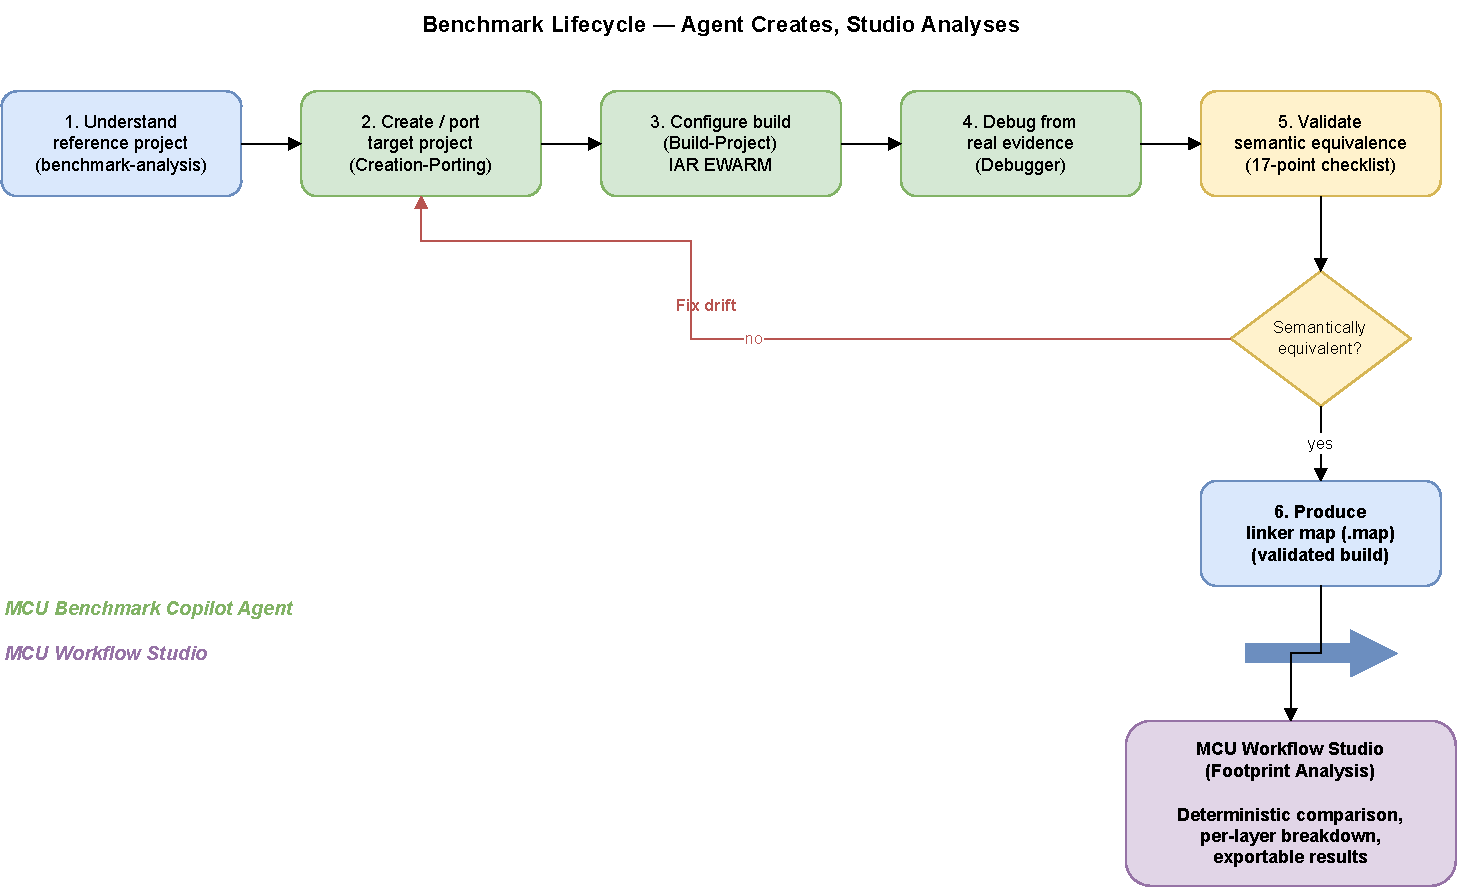
\includegraphics[width=\textwidth]{Figures/benchmark-agent/workflow.pdf}
\caption{End-to-end benchmark lifecycle. The MCU Benchmark Copilot Agent handles steps~1
through~11 autonomously (with a hardware gate at step~9); once semantic equivalence is
confirmed, the validated linker map is handed to MCU Workflow Studio for footprint analysis.}
\label{fig:agent-workflow}
\end{figure}

Figure~\ref{fig:agent-sequence} presents the same campaign as a UML sequence diagram,
showing the actual participant delegation, message flow, the hardware approval gate, and
artifact emission at each step.

\begin{figure}[H]
\centering
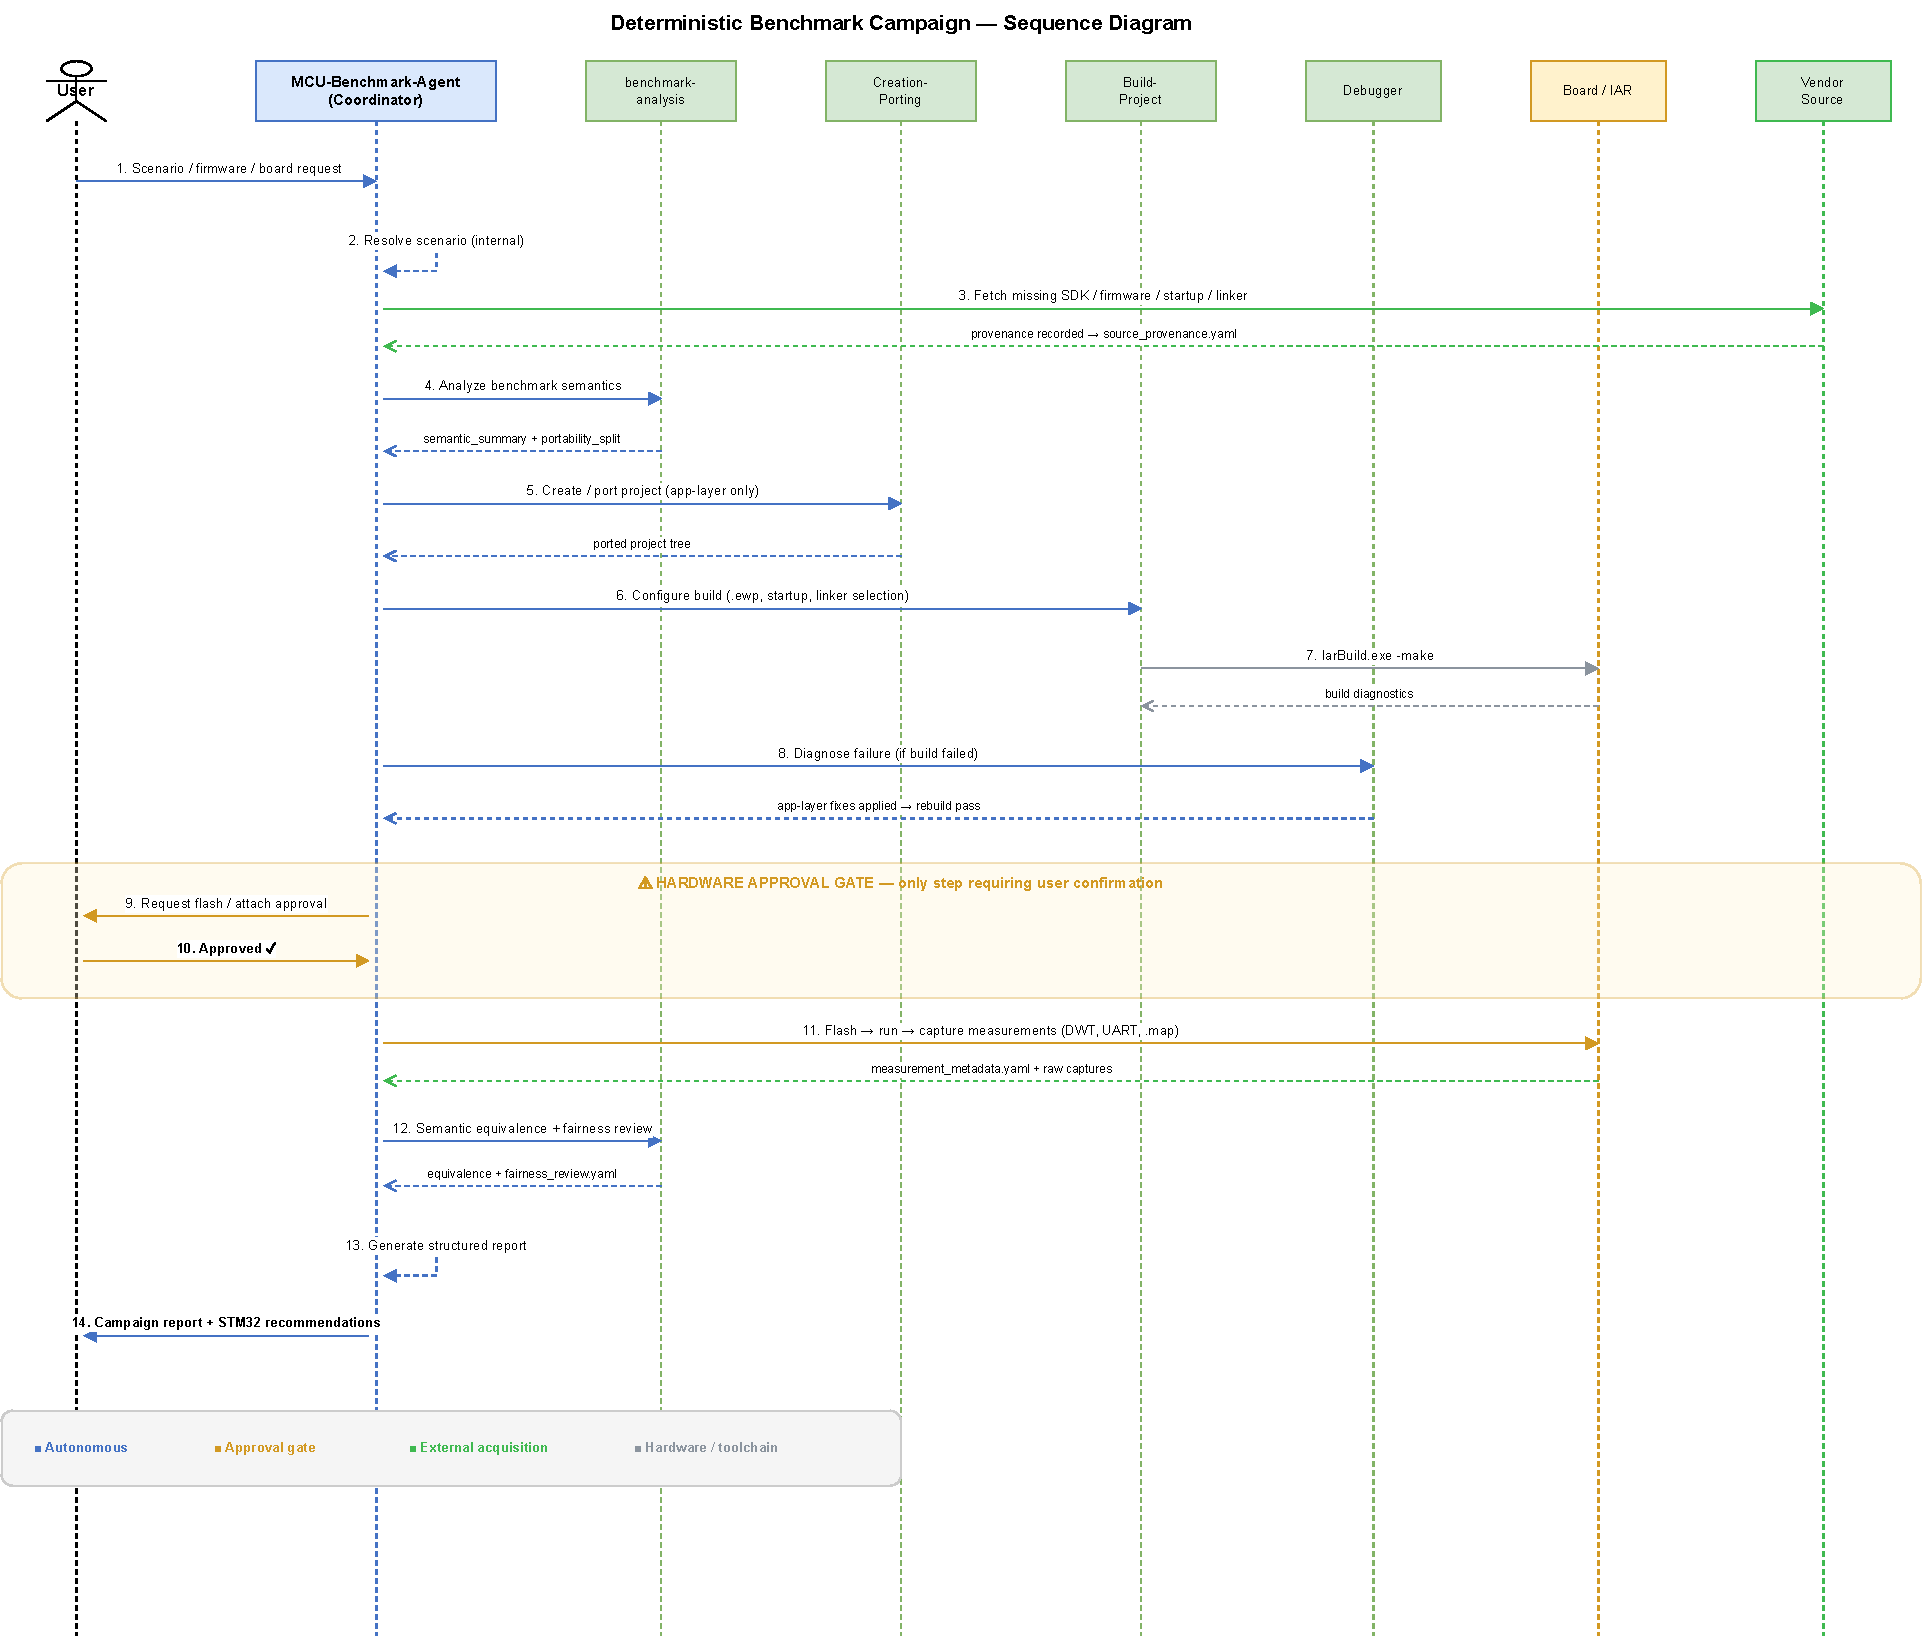
\includegraphics[width=\textwidth]{Figures/benchmark-agent/sequence.pdf}
\caption{UML sequence diagram of a deterministic benchmark campaign. The coordinator
delegates to specialist agents (benchmark-analysis, Creation-Porting, Build-Project,
Debugger) and interacts with external actors (Vendor Source, Board/IAR). The hardware
approval gate (steps~9--10, highlighted) is the only point requiring user confirmation;
all other steps execute autonomously.}
\label{fig:agent-sequence}
\end{figure}

This separation keeps each tool focused. The agent does not attempt footprint analysis, and
the studio does not attempt code generation or debugging. Together, they cover the full
lifecycle of a cross-vendor benchmark: resolve, acquire, create, build, debug, validate,
measure, then analyse.

\section{IAR template resolution}
\label{sec:agent-iar-templates}

Before creating any benchmark project, the system must resolve the correct IAR project
template for the target board. We designed a deterministic four-step resolution algorithm
encoded in the \emph{iar-template-resolution} skill:

\begin{enumerate}
\item \textbf{Exact board match} --- search the template registry (\texttt{iar\_templates.yaml}) for an entry whose \texttt{board\_id} matches the target exactly.
\item \textbf{Family fallback} --- if no exact match, search for a family-level fallback template and adjust device, startup, and linker for the specific MCU.
\item \textbf{Board-type fallback} --- if no family match, select the closest template matching the board type and vendor with explicitly downgraded confidence.
\item \textbf{Unresolved} --- if no suitable template exists, document the gap and report to the user rather than fabricating a template.
\end{enumerate}

When a template is identified but not yet materialised locally, the
\texttt{acquire\_iar\_template.ps1} script fetches it from official vendor GitHub
repositories or SDK packages, records provenance, and verifies the file inventory. The
materialised template then serves as the read-only project baseline into which benchmark
application code is integrated through designated integration points.

\section{Source acquisition policy}
\label{sec:agent-acquisition}

When materials are missing, the agent acquires them autonomously using a strict preference
order:

\begin{enumerate}
\item Workspace files already present.
\item Local SDK content (IAR device/config directories, installed CMSIS packs).
\item Official vendor GitHub repositories (tagged releases preferred).
\item Official vendor websites, SDK packages, CMSIS Pack Index.
\item Third-party mirrors --- only as a last resort, with an explicit risk note.
\end{enumerate}

For every acquired resource, the agent records: source URL, version or branch/tag/commit,
package name, and date of acquisition. This provenance chain ensures that any benchmark
result can be traced back to the exact firmware version used, satisfying the
reproducibility requirements of academic evaluation.

\section{Campaign artifact model}
\label{sec:agent-artifacts}

Each benchmark campaign persists its state in a structured dossier under
\texttt{.github/benchmark/campaigns/<campaign\_id>/}. Key artifacts include:

\begin{itemize}
\item \texttt{campaign\_manifest.yaml} --- campaign identity, platforms, and stage tracking.
\item \texttt{execution\_status.yaml} --- per-stage status with timestamps and blockers.
\item \texttt{source\_provenance.yaml} --- acquisition provenance for every resource used.
\item \texttt{scenario\_resolution.yaml} --- how partial input was resolved.
\item \texttt{fairness\_baseline.yaml} --- per-platform configuration baseline for fairness comparison.
\item \texttt{semantic\_equivalence.yaml} --- verification results per checklist item.
\item \texttt{fairness\_review.yaml} --- all fairness-sensitive differences identified.
\item \texttt{measurement\_metadata.yaml} --- metrics collected, methods, triggers, and confidence levels.
\end{itemize}

This artifact model makes every campaign auditable and reproducible. A reviewer can inspect
the dossier to understand exactly what was resolved, acquired, built, measured, and
concluded --- without re-running the campaign.

\section{Prompt-driven usage}
\label{sec:agent-prompts}

To lower the barrier to entry, the system ships ten pre-built prompt templates
(\texttt{.github/prompts/}) that encode common benchmark tasks. The user selects a prompt
from the Copilot chat picker and fills in minimal parameters (a board name, a scenario, or
a firmware package name); the agent handles everything else. Table~\ref{tab:agent-prompts}
lists the available prompts.

\begin{table}[H]
\centering
\caption{Pre-built prompt templates for common benchmark tasks.}
\label{tab:agent-prompts}
\begin{tabularx}{\textwidth}{c X}
\toprule
\textbf{\#} & \textbf{Purpose} \\
\midrule
01 & Autonomous benchmark from firmware name only --- agent resolves, acquires, builds, and measures. \\
02 & Port a benchmark to another board with fairness guarantee. \\
03 & Build, debug, and measure an existing project autonomously. \\
04 & Compare two boards fairly with semantic-equivalence check. \\
05 & Recommend STM32 improvements after a measured competitor gap. \\
06 & Create a new benchmark from a scenario description (no reference). \\
07 & Port STM32 reference to a competitor platform. \\
08 & Port competitor benchmark to STM32. \\
09 & Port between two non-ST vendors. \\
10 & Resolve and build from a firmware/SDK package name alone. \\
\bottomrule
\end{tabularx}
\end{table}

% TODO(screenshot): Replace placeholder with actual VS Code agent session screenshot
\begin{figure}[H]
\centering
\fbox{\parbox{0.9\textwidth}{\centering\vspace{4cm}\textbf{[PLACEHOLDER --- VS Code agent session screenshot]}\\Capture a VS~Code window showing the Copilot Chat panel with the MCU Benchmark\\Agent active during an autonomous campaign (showing structured output with\\provenance, semantic equivalence, and fairness review).\vspace{4cm}}}
\caption{An autonomous benchmark campaign in VS~Code: the MCU Benchmark Copilot Agent resolves the scenario, acquires firmware, builds, and reports semantic equivalence and fairness status.}
\label{fig:agent-session}
\end{figure}

\section{Implementation}
\label{sec:agent-implementation}

The entire agent system is implemented within a \texttt{.github/} directory, leveraging the
VS Code GitHub Copilot extensibility framework~\cite{github-copilot, vscode-agent-mode,
vscode-custom-agents}.
Agent and skill definitions use YAML frontmatter to declare metadata (name, description,
tool permissions) and Markdown bodies for behavioural instructions. The automation tools are
standalone PowerShell and Python scripts. Table~\ref{tab:agent-impl} summarises the file
structure.

\begin{table}[H]
\centering
\caption{File structure of the agent system.}
\label{tab:agent-impl}
\begin{tabularx}{\textwidth}{l X}
\toprule
\textbf{Path} & \textbf{Role} \\
\midrule
\texttt{.github/copilot-instructions.md} & Always-on rules inherited by every agent and skill. \\
\texttt{.github/agents/*.agent.md} & One file per specialist agent (4 files). \\
\texttt{.github/skills/*/SKILL.md} & One directory per skill, each containing a structured checklist (6 directories). \\
\texttt{.github/tools/*.ps1, *.py} & Twelve automation scripts for deterministic operations. \\
\texttt{.github/config/*.yaml} & Eight configuration registry files (boards, MCUs, vendors, toolchains, templates, sources, measurements, reporting). \\
\texttt{.github/prompts/*.prompt.md} & Ten pre-built prompt templates for common tasks. \\
\texttt{.github/templates/benchmark-dossier/} & Campaign artifact templates (YAML skeletons). \\
\texttt{.github/docs/} & Developer documentation (quickstart, porting guide, validation guide, naming conventions, etc.). \\
\texttt{.github/schemas/} & JSON/YAML schemas for artifact validation. \\
\bottomrule
\end{tabularx}
\end{table}

The implementation requires no external server, no API keys beyond the user's existing
GitHub Copilot subscription, and no deployment pipeline. Adding a new agent, skill, tool,
or board entry is a matter of creating a file and restarting the Copilot Chat session. This
minimal footprint was deliberate: the system should be as easy to maintain and
version-control as the benchmark source code itself.

\section{Integration with the benchmarking workflow}
\label{sec:agent-integration}

The agent system occupies a precise position in the benchmarking pipeline. It sits
\emph{before} MCU Workflow Studio in the workflow: the agent resolves the scenario, acquires
materials, creates and validates the target project, ensures it compiles under IAR EWARM,
confirms that its runtime behaviour matches the reference, and extracts measurements. Only
then does the build's linker map become an input to MCU Workflow Studio for footprint
analysis. The relationship is strictly sequential and complementary --- the agent is
responsible for \emph{producing and validating} correct builds, and the studio is
responsible for \emph{measuring and comparing} them.

\section{Engineering value and limitations}
\label{sec:agent-value}

The agent system's primary value is \emph{autonomous methodology enforcement at scale}. By
encoding the semantic-equivalence checklist, the fairness checklist, the evidence-driven
validation policy, the baseline immutability rule, and the provenance tracking requirement
directly into the tool's behaviour, we ensure that every benchmark campaign follows the
same discipline regardless of which vendor is targeted or how many campaigns run in
parallel.

In practical terms, the agent reduces the time to produce a correct, validated target
project from several hours of manual porting and debugging to an autonomous session
requiring human intervention only at the hardware-programming gate. The deterministic
workflow, the configuration registry, and the campaign artifact model make every result
auditable and reproducible.

The structured output contracts --- each agent returns objective, scenario resolution,
actions executed, semantic equivalence status, fairness status, key findings, unresolved
unknowns, and next action --- make the work transparent and reviewable without re-executing
the campaign.

We acknowledge several limitations. The system depends on the quality of the underlying
language model; while the always-on rules and the configuration registry constrain its
behaviour, they cannot prevent all model errors, particularly for vendor APIs that are
poorly represented in the model's training data. The tool supports IAR EWARM~9.60.3 as the
primary toolchain; extending it to other compilers (GCC, Keil) would require additional
Build-Project configurations and toolchain registry entries. The evidence-driven validation
policy means the system halts at the hardware gate --- it cannot flash a board without
explicit approval. This is by design: in embedded benchmarking, the hardware is the ground
truth, and no amount of static reasoning can substitute for it.

\section*{Conclusion}

We designed and built the MCU Benchmark Copilot Agent as an autonomous campaign coordinator
that fills the engineering gap between defining a benchmark and having a validated,
measured, and fairly compared result. Its four specialist agents cover the full lifecycle
from scenario resolution to measurement extraction; its six reusable skills encode our
methodology as structured checklists; its twelve automation tools provide deterministic
execution; and its configuration registry eliminates hallucination for known hardware facts.
The always-on rules enforce semantic equivalence, benchmark fairness, baseline immutability,
provenance tracking, and evidence-driven validation at every step.

Together with MCU Workflow Studio, the agent forms a complete autonomous toolchain for
reproducible, explainable cross-vendor firmware benchmarking: the agent resolves, acquires,
creates, builds, debugs, validates, and measures; the studio analyses the resulting
footprint. The system supports eight MCU vendors, six workflow directions, and ten
pre-built prompt templates --- making it scalable to the full breadth of the STM32Cube
competitive analysis campaign.

\pagebreak

\chapter{Benchmarking ST against GD32}
\label{chap:vs-gd32}

\section*{Introduction}

GigaDevice Semiconductor is a Chinese fabless semiconductor company that produces the GD32
series of 32-bit microcontrollers \cite{gigadevice-gd32}. The GD32 family is often
positioned as a pin-compatible, drop-in alternative to STM32 parts, sharing the same Arm
Cortex-M cores, similar peripheral sets, and comparable pricing. This close correspondence
makes GD32 a particularly relevant competitor: engineers evaluating an MCU platform
frequently shortlist both vendors, and the choice often comes down to measurable differences
in software-stack quality rather than silicon specifications.

In this chapter we compare the STM32Cube ecosystem against GigaDevice's GD32 firmware
libraries on two middleware stacks: the \textbf{USB device stack} (exercised through HID and
CDC scenarios) and the \textbf{FreeRTOS} real-time operating system integration (exercised
through basic, cooperative, and preemptive scheduling scenarios). For each stack we present
the scenario design, per-scenario footprint and execution-time results, a per-layer ROM
breakdown, and an interpretation of the trade-offs the data reveals.

All measurements follow the methodology described in
Chapter~\ref{chap:general-description}: identical scenarios on both platforms, same compiler
optimisation level, same clock frequency, and results extracted from IAR EWARM linker maps
using the footprint analysis tool presented in Chapter~\ref{chap:footprint-tool}.

% ====================================================================
\section{Hardware platforms}
\label{sec:gd32-boards}

Every scenario in this chapter runs on two boards hosting comparable Cortex-M33 parts: the
STMicroelectronics \textbf{NUCLEO-U575ZI-Q} (STM32U575ZIT6Q) and GigaDevice's
\textbf{GD32E507} evaluation board (GD32E507ZET6). Both devices integrate an Arm Cortex-M33
core clocked at 160\,MHz for these tests, ensuring that performance differences reflect
software-stack efficiency rather than raw silicon speed.
Table~\ref{tab:gd32-boards} contrasts their key characteristics.

\begin{table}[H]
  \centering
  \caption{Board characteristics: ST reference vs GigaDevice GD32.}
  \label{tab:gd32-boards}
  \begin{tabularx}{\textwidth}{l X X}
    \toprule
    \textbf{Characteristic} & \textbf{ST (STM32U575ZIT6Q)} & \textbf{GD32 (GD32E507ZET6)} \\
    \midrule
    Core              & Arm Cortex-M33              & Arm Cortex-M33 \\
    Clock (test)      & 160\,MHz                    & 160\,MHz \\
    Flash             & 2\,MB                       & 512\,KB \\
    SRAM              & 786\,KB                     & 128\,KB \\
    USB               & Full-Speed device            & Full-Speed device \\
    Security          & TrustZone, AES, PKA, HASH    & --- \\
    Toolchain / IDE   & STM32CubeIDE / IAR EWARM     & IAR EWARM \\
    % TODO(source): verify GD32E507 reference price
    \bottomrule
  \end{tabularx}
\end{table}

The STM32U575 belongs to the ultra-low-power STM32U5 series and offers substantially more
flash and RAM, hardware security accelerators, and a richer peripheral set
\cite{stm32u575-ds}. The GD32E507 targets a similar performance point at a competitive
price but with fewer on-chip resources \cite{gigadevice-gd32}. For our benchmarks, the
relevant constant is that \emph{both devices run the same core at the same frequency},
so footprint and execution-time differences are attributable to the vendor's software stack
and HAL implementation.

% ====================================================================
% STACK 1: USB DEVICE STACK
% ====================================================================
\section{USB device stack}
\label{sec:gd32-usb}

The Universal Serial Bus (USB) device stack is a critical middleware component for any MCU
that needs to communicate with a host PC. We benchmark ST's USB Device Library (part of the
STM32Cube middleware) against GigaDevice's USB library, both operating in
\textbf{Full-Speed} mode and running bare-metal (no RTOS).

% --- Scenario design ------------------------------------------------
\subsection{Scenario design}
\label{sec:gd32-usb-scenarios}

We defined two scenarios that cover the most commonly used USB device classes:

\begin{enumerate}
  \item \textbf{HID (Human Interface Device)} --- a low-rate interrupt-transfer scenario in
    which the MCU acts as a USB mouse, sending periodic HID reports to the host. This
    exercises the enumeration path, descriptor handling, and interrupt-endpoint transfer
    logic.
  \item \textbf{CDC (Communication Device Class)} --- a higher-throughput bulk-transfer
    scenario in which the MCU exposes a virtual COM port. The host sends data to the
    device, which echoes it back. This exercises bulk IN/OUT transfers, line-coding
    negotiation, and buffering.
\end{enumerate}

Each scenario was implemented identically on both platforms: same USB descriptors, same
endpoint configuration (Full-Speed), same clock source (internal oscillator ---
HSI48 on STM32, IRC48M on GD32), and same core frequency of 160\,MHz.
Table~\ref{tab:gd32-usb-scenarios} summarises the scenarios and the metrics collected.

\begin{table}[H]
  \centering
  \caption{USB device stack benchmark scenarios.}
  \label{tab:gd32-usb-scenarios}
  \begin{tabularx}{\textwidth}{l X l}
    \toprule
    \textbf{Scenario} & \textbf{What it exercises} & \textbf{Metrics} \\
    \midrule
    HID  & Interrupt transfers, enumeration, descriptor handling
         & ROM/RAM (bytes), init/enum/TX time (ms) \\
    CDC  & Bulk transfers, virtual COM port, echo loopback
         & ROM/RAM (bytes), init/enum/TX/RX time (ms) \\
    \bottomrule
  \end{tabularx}
\end{table}

% --- Results --------------------------------------------------------
\subsection{Results}
\label{sec:gd32-usb-results}

% ---- HID ----------------------------------------------------------
\subsubsection{HID scenario}
\label{sec:gd32-usb-hid}

Table~\ref{tab:gd32-usb-hid-footprint} presents the total ROM and RAM footprint for the
HID scenario.

\begin{table}[H]
  \centering
  \caption{USB HID device footprint (bytes).}
  \label{tab:gd32-usb-hid-footprint}
  \begin{tabular}{l r r r}
    \toprule
    \textbf{Metric} & \textbf{STM32U575} & \textbf{GD32E507} & \textbf{Difference} \\
    \midrule
    ROM (total) & 16\,269 & 9\,175  & $+77\,\%$ \\
    RAM (total) & 3\,446  & 9\,608  & $-65\,\%$ \\
    \bottomrule
  \end{tabular}
\end{table}

The STM32 firmware consumes 77\,\% more ROM than GD32, but uses 65\,\% \emph{less} RAM.
The RAM advantage is substantial: the GD32 implementation requires 0x2000 bytes (8\,KB) of
stack and 0x2000 bytes of heap, whereas the STM32 configuration needs only 0x400 bytes
(1\,KB) of stack and 0x200 bytes (512~bytes) of heap.

Table~\ref{tab:gd32-usb-hid-rom} breaks down the ROM consumption by architectural layer.

\begin{table}[H]
  \centering
  \caption{USB HID ROM breakdown by layer (bytes).}
  \label{tab:gd32-usb-hid-rom}
  \begin{tabular}{l r r r}
    \toprule
    \textbf{Layer} & \textbf{STM32U575} & \textbf{GD32E507} & \textbf{Difference} \\
    \midrule
    Application    & 2\,580  & 1\,942 & $+33\,\%$ \\
    HAL drivers    & 10\,426 & 820    & $+1\,171\,\%$ \\
    MW stack       & 2\,859  & 5\,743 & $-50\,\%$ \\
    \bottomrule
  \end{tabular}
\end{table}

The HAL layer dominates the difference. On STM32, the HAL RCC module alone accounts for
4\,560 bytes (44\,\% of total HAL ROM) and the combined HAL/LL USB driver adds another
4\,988 bytes (48\,\%). By contrast, GD32's HAL layer is minimal at 820 bytes because
GigaDevice folds much of the peripheral-initialisation logic into the middleware itself.
This architectural choice gives GD32 a smaller HAL at the cost of a larger middleware
layer: the GD32 USB library ROM (5\,743 bytes) is twice the size of ST's (2\,859 bytes).

The STM32 application layer is 33\,\% larger because the STM32Cube USB library externalises
device configuration into user files (\texttt{usbd\_desc.c}, \texttt{usbd\_conf.c}),
accounting for 985 bytes (38\,\% of application ROM). On GD32, these configuration concerns
are handled inside the middleware. This design gives STM32 users more configuration
flexibility at the cost of a larger application footprint.

Table~\ref{tab:gd32-usb-hid-exec} shows the execution-time measurements.

\begin{table}[H]
  \centering
  \caption{USB HID execution time (ms).}
  \label{tab:gd32-usb-hid-exec}
  \begin{tabular}{l r r r}
    \toprule
    \textbf{Operation} & \textbf{STM32U575} & \textbf{GD32E507} & \textbf{Difference} \\
    \midrule
    Initialisation      & 9.990  & 26.084 & $-61.7\,\%$ \\
    Enumeration         & 213    & 216    & $-1.4\,\%$ \\
    Data transmission   & 0.0093 & 0.0094 & $-0.7\,\%$ \\
    \bottomrule
  \end{tabular}
\end{table}

The STM32 USB initialisation is 61.7\,\% faster than GD32's --- a significant difference
that reflects more efficient clock-tree configuration and peripheral bring-up in the
STM32Cube HAL. Enumeration and data-transmission times are nearly identical, as expected:
these phases are dominated by USB protocol timing rather than software overhead.

% ---- CDC ----------------------------------------------------------
\subsubsection{CDC scenario}
\label{sec:gd32-usb-cdc}

Table~\ref{tab:gd32-usb-cdc-footprint} presents the total footprint for the CDC scenario.

\begin{table}[H]
  \centering
  \caption{USB CDC device footprint (bytes).}
  \label{tab:gd32-usb-cdc-footprint}
  \begin{tabular}{l r r r}
    \toprule
    \textbf{Metric} & \textbf{STM32U575} & \textbf{GD32E507} & \textbf{Difference} \\
    \midrule
    ROM (total) & 17\,049 & 9\,085  & $+88\,\%$ \\
    RAM (total) & 4\,089  & 9\,683  & $-57.7\,\%$ \\
    \bottomrule
  \end{tabular}
\end{table}

The pattern mirrors HID: STM32 uses substantially more ROM ($+88\,\%$) but far less RAM
($-57.7\,\%$). The CDC scenario adds transmit and receive buffer management, which
increases both vendors' footprints relative to HID, but the ratio remains consistent.

Table~\ref{tab:gd32-usb-cdc-rom} provides the per-layer ROM breakdown.

\begin{table}[H]
  \centering
  \caption{USB CDC ROM breakdown by layer (bytes).}
  \label{tab:gd32-usb-cdc-rom}
  \begin{tabular}{l r r r}
    \toprule
    \textbf{Layer} & \textbf{STM32U575} & \textbf{GD32E507} & \textbf{Difference} \\
    \midrule
    Application    & 2\,683  & 1\,882 & $+42.5\,\%$ \\
    HAL drivers    & 10\,446 & 820    & $+1\,174\,\%$ \\
    MW stack       & 2\,423  & 5\,709 & $-57.5\,\%$ \\
    \bottomrule
  \end{tabular}
\end{table}

The root cause is the same as in HID. The STM32 HAL RCC module (4\,560 bytes) and the
HAL/LL USB driver (5\,006 bytes) together account for 92\,\% of the HAL ROM.
The STM32 application layer is 42.5\,\% larger due to the externalised USB device
configuration files (\texttt{usb\_device.c}, \texttt{usbd\_cdc\_if.c},
\texttt{usbd\_desc.c}, \texttt{usbd\_conf.c}), contributing 1\,164 bytes (43\,\% of
application ROM). In return, the STM32 USB middleware library itself is 57.5\,\% smaller
than GD32's, because GigaDevice bundles configuration and driver logic into its middleware
layer.

Table~\ref{tab:gd32-usb-cdc-exec} shows the execution-time measurements.

\begin{table}[H]
  \centering
  \caption{USB CDC execution time (ms).}
  \label{tab:gd32-usb-cdc-exec}
  \begin{tabular}{l r r r}
    \toprule
    \textbf{Operation} & \textbf{STM32U575} & \textbf{GD32E507} & \textbf{Difference} \\
    \midrule
    Initialisation      & 9.994   & 26.076 & $-61.7\,\%$ \\
    Enumeration         & 218.2   & 218.5  & $-0.1\,\%$ \\
    Data transmission   & 0.00988 & 0.01003 & $-1.5\,\%$ \\
    Data reception      & 0.00986 & 0.00993 & $-0.7\,\%$ \\
    \bottomrule
  \end{tabular}
\end{table}

Once again, initialisation is where STM32 dominates: 61.7\,\% faster than GD32. The
remaining operations (enumeration, transmission, reception) are within 1.5\,\% of each
other, confirming that steady-state USB throughput is protocol-bound rather than
software-bound.

% --- Interpretation -------------------------------------------------
\subsection{Interpretation}
\label{sec:gd32-usb-interp}

The USB benchmark reveals a clear architectural trade-off between the two vendors.

\paragraph{ROM footprint.}
STM32 consumes 77--88\,\% more total ROM than GD32 across both scenarios. The dominant
contributor is the HAL layer, which is roughly twelve times larger on STM32. Two modules
drive this cost: the \textbf{HAL RCC} clock-configuration driver ($\approx$4\,560 bytes)
and the \textbf{HAL/LL USB} peripheral driver ($\approx$5\,000 bytes). GigaDevice achieves
a much smaller HAL by embedding peripheral-initialisation logic inside the middleware
library rather than exposing it as a separate, reusable driver layer.

\paragraph{RAM footprint.}
The situation is reversed: STM32 uses 57--65\,\% less RAM. The GD32 implementation
defaults to much larger stack and heap allocations (8\,KB each vs $\leq$1.5\,KB for STM32).
This suggests that the GD32 USB library relies more heavily on dynamic allocation or deep
call chains, whereas the STM32Cube library uses statically allocated buffers and a
shallower call stack.

\paragraph{Execution time.}
STM32's USB initialisation is consistently 61.7\,\% faster across both HID and CDC. After
initialisation, the two platforms perform within 1--2\,\% of each other, as the USB
protocol itself (enumeration handshake, bulk/interrupt transfers) dictates the timing.

\paragraph{Design philosophy.}
STM32Cube separates concerns: HAL handles clocks and peripheral access, the middleware
handles protocol logic, and the application owns configuration through user-editable files
(\texttt{usbd\_conf.c}, \texttt{usbd\_desc.c}). This modular design gives developers
explicit control and reusability at the cost of a larger total ROM. GigaDevice takes a more
monolithic approach --- smaller HAL, but a thicker middleware that bundles configuration
internally, reducing ROM but also reducing the user's configuration flexibility.

\paragraph{Enhancement proposals.}
The data suggests two concrete areas where STM32Cube could reduce ROM without sacrificing
functionality:

\begin{enumerate}
  \item \textbf{HAL RCC optimisation.} The HAL RCC module accounts for $\approx$4.5\,KB in
    every USB project regardless of the clocks actually configured. A conditionally compiled
    or link-time-optimised RCC driver that includes only the clock paths used would
    significantly narrow the HAL gap.
  \item \textbf{HAL/LL USB driver consolidation.} The combined HAL and LL USB driver
    ($\approx$5\,KB) provides a comprehensive abstraction but may include code paths
    (e.g.\ High-Speed, OTG, DMA) that Full-Speed-only projects never execute. Finer
    compile-time selection of USB features could reduce this cost.
\end{enumerate}

% ====================================================================
% STACK 2: FreeRTOS
% ====================================================================
\section{FreeRTOS integration}
\label{sec:gd32-freertos}

FreeRTOS is the most widely adopted real-time operating system for Cortex-M
microcontrollers \cite{freertos}. Both STMicroelectronics and GigaDevice ship FreeRTOS
integration packages as part of their firmware offerings. We benchmark the two
implementations using FreeRTOS v11.2, running on the same two boards at 160\,MHz with a
1\,ms tick (time slice) per task.

% --- Scenario design ------------------------------------------------
\subsection{Scenario design}
\label{sec:gd32-freertos-scenarios}

We defined three scheduling scenarios that stress progressively more complex RTOS
mechanisms:

\begin{enumerate}
  \item \textbf{Basic processing} --- a single counting thread runs at low priority
    alongside a high-priority reporting thread. The counting thread increments a global
    counter in a tight loop; the reporting thread wakes every 30\,s and prints the counter
    delta. This isolates single-task throughput with minimal scheduler overhead.
  \item \textbf{Cooperative processing} --- five threads at the same low priority, each
    incrementing its own counter and then calling \texttt{taskYIELD()} to voluntarily yield
    the processor. A high-priority reporter prints all five counters every 30\,s. This
    exercises voluntary context switching under equal-priority round-robin scheduling.
  \item \textbf{Preemptive processing} --- five threads at ascending priorities. Each
    thread resumes the next-higher-priority thread (which preempts it), increments its
    counter, then suspends itself. A high-priority reporter prints all five counters every
    30\,s. This exercises the full preemptive scheduler: suspend, resume, and
    priority-based preemption.
\end{enumerate}

Table~\ref{tab:gd32-freertos-scenarios} summarises the three scenarios.

\begin{table}[H]
  \centering
  \caption{FreeRTOS benchmark scenarios.}
  \label{tab:gd32-freertos-scenarios}
  \begin{tabularx}{\textwidth}{l X l}
    \toprule
    \textbf{Scenario} & \textbf{What it exercises} & \textbf{Metric} \\
    \midrule
    Basic        & Single-thread throughput, minimal scheduler overhead
                 & Thread iterations/s \\
    Cooperative  & Voluntary context switching (\texttt{taskYIELD})
                 & Total thread iterations/30\,s \\
    Preemptive   & Priority-based preemption, suspend/resume
                 & Total thread iterations/30\,s \\
    \bottomrule
  \end{tabularx}
\end{table}

% --- Results --------------------------------------------------------
\subsection{Results}
\label{sec:gd32-freertos-results}

% ---- Basic processing ---------------------------------------------
\subsubsection{Basic processing}
\label{sec:gd32-freertos-basic}

Table~\ref{tab:gd32-freertos-basic-perf} shows the performance result and
Table~\ref{tab:gd32-freertos-basic-fp} the footprint.

\begin{table}[H]
  \centering
  \caption{FreeRTOS basic processing --- performance.}
  \label{tab:gd32-freertos-basic-perf}
  \begin{tabular}{l r r r}
    \toprule
    \textbf{Metric} & \textbf{STM32U575} & \textbf{GD32E507} & \textbf{Difference} \\
    \midrule
    Thread iterations/s & 47\,943 & 47\,955 & $-0.025\,\%$ \\
    \bottomrule
  \end{tabular}
\end{table}

\begin{table}[H]
  \centering
  \caption{FreeRTOS basic processing --- footprint (bytes).}
  \label{tab:gd32-freertos-basic-fp}
  \begin{tabular}{l r r r}
    \toprule
    \textbf{Metric} & \textbf{STM32U575} & \textbf{GD32E507} & \textbf{Difference} \\
    \midrule
    ROM & 14\,266 & 10\,128 & $+40.9\,\%$ \\
    RAM & 11\,960 & 11\,716 & $+2.1\,\%$ \\
    \bottomrule
  \end{tabular}
\end{table}

Performance is virtually identical ($-0.025\,\%$), confirming that the counting loop is
CPU-bound and both FreeRTOS ports schedule it with the same efficiency. The ROM difference
($+40.9\,\%$) is significant; the RAM difference is negligible.

% ---- Cooperative processing ----------------------------------------
\subsubsection{Cooperative processing}
\label{sec:gd32-freertos-coop}

\begin{table}[H]
  \centering
  \caption{FreeRTOS cooperative processing --- performance.}
  \label{tab:gd32-freertos-coop-perf}
  \begin{tabular}{l r r r}
    \toprule
    \textbf{Metric} & \textbf{STM32U575} & \textbf{GD32E507} & \textbf{Difference} \\
    \midrule
    Thread iterations/30\,s & 1\,220\,066 & 1\,200\,666 & $+1.6\,\%$ \\
    \bottomrule
  \end{tabular}
\end{table}

\begin{table}[H]
  \centering
  \caption{FreeRTOS cooperative processing --- footprint (bytes).}
  \label{tab:gd32-freertos-coop-fp}
  \begin{tabular}{l r r r}
    \toprule
    \textbf{Metric} & \textbf{STM32U575} & \textbf{GD32E507} & \textbf{Difference} \\
    \midrule
    ROM & 15\,422 & 11\,224 & $+37\,\%$ \\
    RAM & 10\,972 & 10\,728 & $+2.3\,\%$ \\
    \bottomrule
  \end{tabular}
\end{table}

STM32 completes 1.6\,\% more thread iterations over 30 seconds, indicating a marginally
faster \texttt{taskYIELD()} context switch. The footprint gap narrows slightly to
$+37\,\%$ ROM.

% ---- Preemptive processing -----------------------------------------
\subsubsection{Preemptive processing}
\label{sec:gd32-freertos-preemptive}

\begin{table}[H]
  \centering
  \caption{FreeRTOS preemptive processing --- performance.}
  \label{tab:gd32-freertos-preemptive-perf}
  \begin{tabular}{l r r r}
    \toprule
    \textbf{Metric} & \textbf{STM32U575} & \textbf{GD32E507} & \textbf{Difference} \\
    \midrule
    Thread iterations/30\,s & 294\,615 & 285\,144 & $+3.3\,\%$ \\
    \bottomrule
  \end{tabular}
\end{table}

\begin{table}[H]
  \centering
  \caption{FreeRTOS preemptive processing --- footprint (bytes).}
  \label{tab:gd32-freertos-preemptive-fp}
  \begin{tabular}{l r r r}
    \toprule
    \textbf{Metric} & \textbf{STM32U575} & \textbf{GD32E507} & \textbf{Difference} \\
    \midrule
    ROM & 16\,226 & 12\,028 & $+35\,\%$ \\
    RAM & 10\,996 & 10\,748 & $+2.3\,\%$ \\
    \bottomrule
  \end{tabular}
\end{table}

Preemptive scheduling is the most demanding scenario, involving suspend, resume, and
priority-based task switching. STM32 achieves 3.3\,\% more iterations, the largest
performance advantage across the three FreeRTOS scenarios. The ROM gap ($+35\,\%$) is
consistent with the other scenarios.

% ---- Per-layer ROM breakdown (all three scenarios) -----------------
\subsubsection{Per-layer ROM breakdown}
\label{sec:gd32-freertos-rom-breakdown}

To understand \emph{where} the ROM overhead originates, Table~\ref{tab:gd32-freertos-rom}
breaks down the ROM footprint into three architectural layers --- application, HAL drivers,
and FreeRTOS middleware stack --- for all three scenarios.

\begin{table}[H]
  \centering
  \caption{FreeRTOS ROM breakdown by layer (bytes).}
  \label{tab:gd32-freertos-rom}
  \begin{tabular}{l l r r r}
    \toprule
    \textbf{Scenario} & \textbf{Layer} & \textbf{STM32U575} & \textbf{GD32E507}
        & \textbf{Diff.} \\
    \midrule
    \multirow{3}{*}{Basic}
      & Application & 4\,531  & 4\,278 & $+6\,\%$ \\
      & HAL drivers & 4\,927  & 1\,078 & $+357\,\%$ \\
      & MW stack    & 4\,808  & 4\,772 & $+0.7\,\%$ \\
    \midrule
    \multirow{3}{*}{Cooperative}
      & Application & 5\,823  & 5\,484 & $+6\,\%$ \\
      & HAL drivers & 4\,911  & 1\,078 & $+355\,\%$ \\
      & MW stack    & 4\,688  & 4\,662 & $+0.6\,\%$ \\
    \midrule
    \multirow{3}{*}{Preemptive}
      & Application & 6\,191  & 5\,810 & $+6\,\%$ \\
      & HAL drivers & 4\,911  & 1\,078 & $+355\,\%$ \\
      & MW stack    & 5\,124  & 5\,140 & $-0.3\,\%$ \\
    \bottomrule
  \end{tabular}
\end{table}

The pattern is strikingly consistent across all three scenarios:

\begin{itemize}
  \item The \textbf{FreeRTOS middleware stack} itself is virtually identical in size
    ($\leq$1\,\% difference). Both vendors ship the same upstream FreeRTOS kernel, so
    this is expected.
  \item The \textbf{application layer} is $\approx$6\,\% larger on STM32, reflecting
    slightly more initialisation code in the STM32Cube project template.
  \item The \textbf{HAL layer} is 355--357\,\% larger on STM32, entirely accounting for
    the total ROM gap. The dominant contributor is the \textbf{HAL RCC} module, which
    configures the clock tree.
\end{itemize}

% --- Interpretation -------------------------------------------------
\subsection{Interpretation}
\label{sec:gd32-freertos-interp}

\paragraph{Performance.}
FreeRTOS scheduling performance is nearly identical between the two platforms in the basic
scenario ($-0.025\,\%$) and slightly favours STM32 in the cooperative ($+1.6\,\%$) and
preemptive ($+3.3\,\%$) scenarios. The advantage grows with scheduler complexity, suggesting
that the STM32Cube FreeRTOS port has a marginally more efficient context-switch
implementation. However, these differences are small enough that application-level
performance is unlikely to be affected.

\paragraph{ROM footprint.}
The ROM overhead follows the same pattern as the USB stack: a 35--41\,\% total increase
driven almost entirely by the HAL layer, specifically the HAL RCC clock-configuration
module. Crucially, the FreeRTOS middleware itself contributes no measurable overhead ---
the gap is in the vendor's hardware-abstraction code, not in the RTOS kernel.

\paragraph{RAM footprint.}
RAM differences are negligible (2.1--2.3\,\%), indicating that both FreeRTOS ports allocate
task stacks and kernel structures similarly.

\paragraph{Enhancement proposals.}
The FreeRTOS results reinforce the conclusion from the USB benchmark: the HAL RCC module
is the single largest contributor to STM32's ROM overhead across \emph{all} middleware
stacks. A targeted effort to slim the RCC driver --- through dead-code elimination,
conditional compilation based on the clocks actually used, or link-time optimisation ---
would benefit every STM32 project, not just FreeRTOS.

% ====================================================================
\section*{Conclusion}

The ST-versus-GD32 comparison across two middleware stacks (USB device and FreeRTOS) and
five scenarios reveals a consistent pattern:

\begin{itemize}
  \item \textbf{Performance:} STM32 matches or slightly exceeds GD32 in every scenario.
    USB initialisation is 61.7\,\% faster; FreeRTOS preemptive scheduling is 3.3\,\% faster;
    steady-state throughput is equivalent.
  \item \textbf{ROM footprint:} STM32 consumes 35--88\,\% more flash, with the HAL layer
    (principally HAL RCC and, for USB, HAL/LL USB) responsible for the bulk of the
    difference. The middleware stacks themselves are comparable in size.
  \item \textbf{RAM footprint:} STM32 uses significantly less RAM than GD32 in USB
    scenarios (57--65\,\% less) thanks to smaller default stack/heap allocations and more
    static memory management. FreeRTOS RAM is nearly identical.
  \item \textbf{Architectural trade-off:} STM32Cube's modular, layered design (separate
    HAL, middleware, and user-configuration files) provides greater flexibility and
    reusability but at a measurable ROM cost. GigaDevice's more monolithic approach yields
    smaller ROM by bundling driver and configuration logic into the middleware, at the
    expense of less user-visible modularity.
\end{itemize}

The single most impactful enhancement for STM32 would be \textbf{optimising the HAL RCC
module}: it appears in every project and consistently accounts for the largest share of the
HAL ROM gap. A secondary improvement for USB projects would be \textbf{finer-grained
compile-time selection} of USB driver features (Full-Speed vs High-Speed, device vs OTG)
to exclude unused code paths.

\pagebreak

\chapter{Benchmarking ST against Texas Instruments}
\label{chap:vs-ti}

\section*{Introduction}

Texas Instruments (TI) is one of the world's largest semiconductor manufacturers, with a
broad portfolio of embedded processors and microcontrollers~\cite{ti-about}. Its MSPM0 and
MSPM3 families, built around Arm Cortex-M0+ and Cortex-M33 cores respectively, target
cost-sensitive and mixed-signal applications with a strong emphasis on analog
integration~\cite{ti-mspm33-product}. Unlike GigaDevice, which competes primarily on
pin-compatibility, TI competes on a fundamentally different SDK architecture: a
SysConfig-centric, unified serial peripheral model and a single-layer driver library
(driverlib) rather than the dual HAL/LL approach used by STMicroelectronics.

This chapter presents the first phase of our ST-versus-TI comparison: a comprehensive
\textbf{static analysis} of the low-level driver layers of both SDKs. Unlike the
runtime-focused benchmarks in Chapter~\ref{chap:vs-gd32}, this analysis examines source-code
quality and SDK breadth without executing firmware on hardware. We compare the
STM32CubeC5 Low-Layer (LL) drivers~\cite{stm32cubec5-sw} against the TI MSPM33 SDK
driverlib~\cite{ti-mspm33-sdk} across seven quality dimensions --- lines of code,
documentation coverage, code duplication, cyclomatic complexity, API surface design,
MISRA~C:2012 compliance, and security (CWE analysis). For the scope definition, we also
map the SDK coverage in terms of peripheral drivers, middleware, cryptographic algorithms,
and communication protocols, identifying what each vendor offers exclusively.

All measurements were produced by automated scripts using
\texttt{cloc}~\cite{cloc-tool}, \texttt{cppcheck}~\cite{cppcheck-tool} (with its
\texttt{--addon=misra} and \texttt{--addon=cert} modes),
\texttt{lizard}~\cite{lizard-tool} for cyclomatic complexity, and
\texttt{jscpd}~\cite{jscpd-tool} for duplication detection.

% ====================================================================
\section{Hardware platforms}
\label{sec:ti-boards}

The analysis in this chapter targets driver code for two boards hosting comparable
Cortex-M33 parts. Table~\ref{tab:ti-board-comparison} summarises their key characteristics.

\begin{table}[H]
\centering
\caption{Board and MCU comparison --- STM32C5A3 vs.\ MSPM33C321A.}
\label{tab:ti-board-comparison}
\begin{tabular}{l l l}
\toprule
\textbf{Feature} & \textbf{STM32C5A3 (NUCLEO-C5A3ZG)} & \textbf{MSPM33C321A (LP-MSPM33C321A)} \\
\midrule
Core & Arm Cortex-M33 (FPU, DSP, MPU) & Arm Cortex-M33 (FPU, DSP, TrustZone) \\
Max frequency & 144\,MHz & 160\,MHz \\
Flash & 1\,MB (ECC, dual-bank) & 1\,MB (ECC, dual-bank, address swap) \\
SRAM & 256\,KB (128\,KB with ECC) & 256\,KB (ECC) \\
ADC & 3 $\times$ 12-bit, 4.5\,MSPS & 2 $\times$ 12-bit, 9.4\,MSPS \\
DAC & 1 $\times$ 12-bit & 2 $\times$ 8-bit \\
CAN & 2 $\times$ FDCAN & 2 $\times$ CAN\,FD \\
USB & USB\,2.0 FS (Host/Device/DRD) & --- \\
Ethernet & Yes (MAC with DMA) & --- \\
I3C & Yes & --- \\
Debug probe & ST-LINK & XDS110 (EnergyTrace) \\
\bottomrule
\end{tabular}
\end{table}

Both parts share the same core architecture and identical flash/RAM capacities, which makes
the comparison fair at the silicon level. The STM32C5A3 offers broader connectivity (USB,
Ethernet, I3C), while the MSPM33C321A favours higher analog bandwidth (9.4\,MSPS ADC) and
provides TrustZone support~\cite{ti-mspm33-ds,stm32c5a3-product}.

% ====================================================================
\section{Static analysis of the driver layer}
\label{sec:ti-static-analysis}

This section compares the LL driver layer of STM32CubeC5 against the driverlib of the
MSPM33 SDK. The LL layer was chosen for ST because it is the closest architectural
equivalent to TI's driverlib: both are thin, inline-heavy abstractions over peripheral
registers, designed for performance-critical code. We analyse seven complementary
dimensions.

% --------------------------------------------------------------------
\subsection{Scope and methodology}
\label{subsec:ti-scope}

The analysis targets the following source sets:

\begin{itemize}
  \item \textbf{ST:} all 33 header files in
        \texttt{stm32c5xx\_drivers/ll/} (the LL layer of STM32CubeC5).
  \item \textbf{TI:} all 85 source and header files in
        \texttt{source/ti/driverlib/} and its \texttt{m33/} subdirectory
        (the driverlib of MSPM33 SDK v1.03.00.01).
\end{itemize}

Both sets were analysed on the same workstation under identical tool configurations. The
tools and their roles are:

\begin{itemize}
  \item \textbf{cloc} v2.08~\cite{cloc-tool} --- counts blank, comment, and code lines per
        language and file.
  \item \textbf{lizard}~\cite{lizard-tool} --- computes cyclomatic complexity, number of
        parameters, and token count per function.
  \item \textbf{cppcheck} v2.x~\cite{cppcheck-tool} --- runs MISRA~C:2012 addon
        (\texttt{--addon=misra}) and CWE/CERT checks.
  \item \textbf{jscpd}~\cite{jscpd-tool} --- detects copy-pasted code blocks (duplication).
  \item A custom Python script (\texttt{analyze\_firmware.py}) --- extracts API surface
        metrics (public/static/inline functions, macros, enums, naming patterns, parameter
        distributions) and documentation coverage (Doxygen blocks, \texttt{@brief},
        \texttt{@param}, \texttt{@return} tags, file headers).
\end{itemize}

% --------------------------------------------------------------------
\subsection{Lines of code}
\label{subsec:ti-loc}

Table~\ref{tab:ti-loc} presents the line-count breakdown for each SDK's driver layer.

\begin{table}[H]
\centering
\caption{Lines-of-code comparison --- ST LL vs.\ TI driverlib.}
\label{tab:ti-loc}
\begin{tabular}{l r r}
\toprule
\textbf{Metric} & \textbf{ST (LL)} & \textbf{TI (driverlib)} \\
\midrule
Source files      &        33 &        85 \\
Blank lines       &     5\,744 &     8\,747 \\
Comment lines     &    57\,649 &    45\,763 \\
Code lines        &    22\,292 &    27\,972 \\
\midrule
Total lines       &    85\,685 &    82\,482 \\
Comment-to-code ratio & 2.59 & 1.64 \\
\bottomrule
\end{tabular}
\end{table}

ST delivers its LL layer in 33 header-only files containing 22\,292 lines of code, while
TI spreads its driverlib across 85 files (both \texttt{.c} and \texttt{.h}) with
27\,972 code lines. Despite having 25\% more code, TI's total line count is slightly
lower because ST invests significantly more in inline comments: 57\,649 comment lines
versus 45\,763, yielding a comment-to-code ratio of 2.59 for ST compared with 1.64 for TI.
This difference reflects ST's header-only, fully-documented inline function strategy, where
each function carries extensive Doxygen annotations embedded alongside the implementation.

% --------------------------------------------------------------------
\subsection{Documentation coverage}
\label{subsec:ti-doc}

We measured documentation quality through Doxygen tag extraction.
Table~\ref{tab:ti-doc} summarises the results.

\begin{table}[H]
\centering
\caption{Documentation coverage --- ST LL vs.\ TI driverlib.}
\label{tab:ti-doc}
\begin{tabular}{l r r}
\toprule
\textbf{Metric} & \textbf{ST (LL)} & \textbf{TI (driverlib)} \\
\midrule
Total functions         &   3\,713 &   3\,056 \\
Documented functions    &   3\,613 &   2\,525 \\
\textbf{Doc.\ coverage} & \textbf{97.3\,\%} & \textbf{82.6\,\%} \\
\midrule
Doxygen blocks          &   5\,967 &   3\,357 \\
\texttt{@brief} tags    &   3\,826 &   5\,568 \\
\texttt{@param} tags    &   4\,440 &   3\,970 \\
\texttt{@return} tags   &   1\,705 &   2\,172 \\
File headers            &      33  &      85  \\
Inline comments         &       0  &     283  \\
\bottomrule
\end{tabular}
\end{table}

ST achieves 97.3\% function-level documentation coverage, leaving only 100 undocumented
functions. TI reaches 82.6\%, with 531 undocumented functions --- mostly in \texttt{.c}
implementation files, where TI concentrates complex logic (e.g.\ flash controller
operations, PLL configuration) without per-function Doxygen blocks. This architectural
choice is deliberate: TI documents the \emph{header} API thoroughly but omits Doxygen in
\texttt{.c} bodies, whereas ST's header-only approach means every function definition is
also its documented declaration.

Interestingly, TI uses more \texttt{@brief} tags (5\,568 vs.\ 3\,826) and more
\texttt{@return} tags (2\,172 vs.\ 1\,705), suggesting that when TI does document a
function, it tends to be descriptive about purpose and return values. ST, however, produces
78\% more Doxygen blocks overall (5\,967 vs.\ 3\,357), reflecting its higher raw volume of
documented entities.

% --------------------------------------------------------------------
\subsection{Code duplication}
\label{subsec:ti-dup}

Table~\ref{tab:ti-dup} presents the duplication metrics.

\begin{table}[H]
\centering
\caption{Code duplication --- ST LL vs.\ TI driverlib.}
\label{tab:ti-dup}
\begin{tabular}{l r r}
\toprule
\textbf{Metric} & \textbf{ST (LL)} & \textbf{TI (driverlib)} \\
\midrule
Total lines analysed     &    85\,685 &    82\,403 \\
Code lines               &    10\,461 &    18\,008 \\
Duplicate blocks         &        71 &       414 \\
Duplicate lines          &       229 &     1\,306 \\
\textbf{Duplication \%}  & \textbf{2.19\,\%} & \textbf{7.25\,\%} \\
\midrule
Same-file clones         &        71 &       338 \\
Cross-file clones        &         0 &        76 \\
\bottomrule
\end{tabular}
\end{table}

TI's driver layer exhibits 3.3$\times$ more duplication than ST's (7.25\% vs.\ 2.19\%).
All 71 duplicate blocks in ST occur within the same file, typically in symmetric
getter/setter pairs for multi-channel peripherals (e.g.\ ADC rank configuration).
TI, by contrast, has 76 cross-file clones --- code that is structurally identical across
different peripheral modules. This pattern arises from TI's UniComm architecture, where
\texttt{dl\_unicommuart.h}, \texttt{dl\_unicommspi.h}, and \texttt{dl\_unicommi2cc.h}
share a common General Serial Controller (GSC) base but replicate similar interrupt-handling
and configuration boilerplate in each specialisation.

The higher duplication in TI is not inherently a quality defect --- it reflects a design
choice that trades some code reuse for peripheral-specific readability. However, from a
maintenance perspective, ST's lower duplication means fewer locations to update when fixing
a bug or adapting to silicon errata.

% --------------------------------------------------------------------
\subsection{Cyclomatic complexity}
\label{subsec:ti-complexity}

Cyclomatic complexity (CC) measures the number of linearly independent paths through a
function; higher values indicate more decision branches and, consequently, harder-to-test
code~\cite{lizard-tool}. We ran Lizard on every function in both driver sets and
summarise the results in Table~\ref{tab:ti-complexity}.

\begin{table}[H]
\centering
\caption{Cyclomatic complexity comparison --- ST LL vs.\ TI driverlib.}
\label{tab:ti-complexity}
\begin{tabular}{l r r}
\toprule
\textbf{Metric} & \textbf{ST (LL)} & \textbf{TI (driverlib)} \\
\midrule
Analysed functions       &    3\,542 &    2\,539 \\
Mean CC                  &      4.44 &      7.35 \\
Median CC                &         4 &         5 \\
Maximum CC               &        49 &       141 \\
\midrule
Functions with CC $>$ 10 &    44 \scriptsize(1.2\,\%) &   335 \scriptsize(13.2\,\%) \\
Functions with CC $>$ 20 &    12 \scriptsize(0.3\,\%) &    97 \scriptsize(3.8\,\%) \\
\bottomrule
\end{tabular}
\end{table}

ST's driver code is markedly flatter: the average function has fewer than five decision
points, and only 1.2\,\% of functions exceed the widely accepted threshold of
CC\,=\,10~\cite{misra-c2012}. The maximum (CC\,=\,49) occurs in a temperature-calculation
helper (\texttt{LL\_ADC\_CALC\_TEMPERATURE}) that contains a long chain of calibration
look-ups.

TI's SDK shows a heavier tail: 13.2\,\% of its functions exceed CC\,=\,10, with a peak of
141 in a single function. Many of these high-complexity functions reside in the UniComm
serial-controller layer, where a large \texttt{switch} dispatches configuration variants
for UART, SPI, and I\textsuperscript{2}C through a shared code path. While this design
consolidates peripheral logic, it concentrates branching in ways that complicate unit testing
and formal verification.

From a maintainability standpoint, ST's approach of decomposing peripheral logic into many
small, low-complexity inline functions aligns better with safety-coding guidelines that
recommend CC\,$\leq$\,10 per function.

% --------------------------------------------------------------------
\subsection{API surface}
\label{subsec:ti-api}

Table~\ref{tab:ti-api} compares the API design characteristics.

\begin{table}[H]
\centering
\caption{API surface comparison --- ST LL vs.\ TI driverlib.}
\label{tab:ti-api}
\begin{tabular}{l r r}
\toprule
\textbf{Metric} & \textbf{ST (LL)} & \textbf{TI (driverlib)} \\
\midrule
Public functions         &    3\,543 &    2\,500 \\
Static functions         &         1 &        42 \\
Inline functions         &    3\,543 &    2\,032 \\
Functional macros        &       194 &        27 \\
Constant macros          &     3\,993 &    3\,271 \\
Enums                    &         1 &       361 \\
Typedefs                 &         0 &       470 \\
\midrule
Avg.\ parameters/func.  &      1.17 &      1.69 \\
Max parameters           &         8 &         8 \\
\texttt{extern "C"} guards &    33 &        43 \\
Include guards           &        33 &         0 \\
\midrule
\multicolumn{3}{l}{\textbf{Parameter distribution (functions by param count)}} \\
0 parameters             &       492 &       120 \\
1 parameter              &     2\,303 &     1\,160 \\
2 parameters             &       658 &       933 \\
3 parameters             &       135 &       274 \\
4+ parameters            &        48 &       139 \\
\bottomrule
\end{tabular}
\end{table}

The two APIs reflect fundamentally different design philosophies:

\begin{itemize}
  \item \textbf{ST LL} exposes 3\,543 public functions, \emph{all} of which are
        \texttt{\_\_STATIC\_INLINE}. The API is almost entirely composed of one-parameter
        getters and zero-parameter status queries (65\% of functions take 0 or 1 parameter).
        Type safety relies on constant macros rather than enums. The naming convention
        follows the \texttt{LL\_PERIPHERAL\_Action} pattern consistently across all 33
        files.
  \item \textbf{TI driverlib} exposes 2\,500 public functions, of which 2\,032 are inline
        (81\%). It makes heavier use of enums (361 enum types) and typedefs (470) for
        configuration parameters, which improves type safety and IDE autocompletion at the
        cost of a more complex type graph. The naming convention follows
        \texttt{DL\_Peripheral\_Action} uniformly. Functions tend to take more parameters
        on average (1.69 vs.\ 1.17), reflecting a more configuration-object-oriented
        style where a single call sets multiple related fields.
\end{itemize}

ST's 194 functional macros versus TI's 27 show that ST still uses preprocessor computation
in places (e.g.\ register-offset calculations, bit-field assembly) where TI has migrated
the same logic into inline functions. While both approaches compile to equivalent machine
code, the inline-function approach provides better debugging and type checking.

% --------------------------------------------------------------------
\subsection{MISRA~C:2012 compliance}
\label{subsec:ti-misra}

Both SDKs were analysed using \texttt{cppcheck} with the MISRA~C:2012
addon~\cite{misra-c2012}. Table~\ref{tab:ti-misra} presents the per-rule breakdown.

\begin{table}[H]
\centering
\caption{MISRA~C:2012 violations --- ST LL vs.\ TI driverlib.}
\label{tab:ti-misra}
\begin{tabular}{l l r r}
\toprule
\textbf{Rule} & \textbf{Description} & \textbf{ST} & \textbf{TI} \\
\midrule
17.3 & Function declared implicitly       & 3\,541 &  281 \\
11.4 & Conversion between pointer and integer & 84 &    4 \\
10.6 & Composite expression assigned to wider type & 29 & --- \\
20.7 & Macro parameter not enclosed in parentheses & 21 & --- \\
7.3  & Lower-case ``l'' suffix on literal  &    18 & --- \\
10.4 & Incompatible essential types in operation & --- & 67 \\
12.1 & Precedence of operators unclear     & --- &   52 \\
18.4 & Pointer arithmetic                  & --- &   76 \\
15.5 & Multiple return statements          &     4 &   14 \\
10.1 & Operands of inappropriate essential type & --- & 13 \\
3.1  & Comment contains nested comment     & --- &   11 \\
Other & Various minor rules                &    6 &   33 \\
\midrule
\textbf{Total} & & \textbf{3\,703} & \textbf{551} \\
\bottomrule
\end{tabular}
\end{table}

\subsubsection*{Interpretation}
At first glance, ST's LL layer appears to have far more MISRA violations (3\,703 vs.\ 551).
However, this requires careful interpretation:

\begin{enumerate}
  \item \textbf{Rule 17.3 dominates ST's count.} Of ST's 3\,703 violations, 3\,541 (96\%)
        are Rule~17.3 (implicit function declaration). These arise because every LL
        function is defined as \texttt{\_\_STATIC\_INLINE} in a header and \texttt{cppcheck}
        analyses each header in isolation, reporting each inline function call within the
        same header as an implicit declaration when the callee is defined later in the file.
        In a real compilation unit (where the header is \texttt{\#include}d), these are all
        resolved. This is a \emph{tooling artifact}, not a genuine code-quality issue.

  \item \textbf{Rule 11.4 is unavoidable in MCU drivers.} The 84 Rule~11.4 violations in ST
        are casts between integers and peripheral base-address pointers
        (\texttt{(ADC\_TypeDef~*)ADC1\_BASE}). Both vendors do this; TI has the same
        pattern but fewer instances (4) because TI defines peripheral pointers via
        device-header macros that \texttt{cppcheck} does not fully expand.

  \item \textbf{TI's violations are more diverse.} TI triggers 15 distinct MISRA rules
        compared with ST's 9. Rules 18.4 (pointer arithmetic, 76 occurrences), 10.4
        (essential-type mismatch, 67), and 12.1 (operator precedence, 52) point to more
        complex expression patterns in TI's \texttt{.c} implementation files.
\end{enumerate}

\noindent
If we exclude the tooling-artifact Rule~17.3 from both vendors, the adjusted counts are
ST~=~162 and TI~=~270, putting ST ahead on genuine MISRA conformance per line of code.

\subsubsection*{Security analysis (CWE)}
Both driver layers returned \textbf{zero CWE findings} from \texttt{cppcheck}'s CERT/CWE
checker. Neither SDK contains patterns flagged as common weakness enumerations, which is
expected for thin, register-level driver code that performs no dynamic allocation, string
handling, or network I/O.

% ====================================================================
\section{SDK coverage comparison}
\label{sec:ti-sdk-coverage}

Beyond driver-layer quality, the breadth of an SDK --- how many peripherals, middleware
stacks, and communication protocols it supports out of the box --- determines the
development effort required for a real product. We mapped the complete contents of both
SDKs file by file and identified exclusive features on each side.

% --------------------------------------------------------------------
\subsection{Peripheral driver coverage}
\label{subsec:ti-periph-gaps}

Table~\ref{tab:ti-periph-exclusive} lists the peripheral drivers present in only one
SDK.\footnote{For brevity, only a representative subset of ST's 25 exclusive drivers is
shown; the full list is available in the analysis output.}

\begin{table}[H]
\centering
\caption{Exclusive peripheral drivers --- features in one SDK only.}
\label{tab:ti-periph-exclusive}
\begin{tabular}{l p{5.5cm} l}
\toprule
\textbf{Vendor} & \textbf{Driver} & \textbf{Capability} \\
\midrule
\multicolumn{3}{l}{\textit{ST-exclusive (25 drivers)}} \\
ST & CORDIC accelerator              & HW trigonometric/hyperbolic math \\
ST & DAC (12-bit)                    & Full DAC peripheral \\
ST & Ethernet MAC                    & On-chip networking \\
ST & USB Host / Device / DRD         & Full USB stack support \\
ST & I3C controller                  & Next-gen I3C bus \\
ST & HASH accelerator (SHA)          & HW SHA-1/SHA-256 \\
ST & OPAMP                           & On-chip operational amplifier \\
ST & ICACHE controller               & Configurable instruction cache \\
ST & XSPI (Octo/Quad-SPI)           & Advanced memory-mapped SPI \\
ST & LPUART, USART, SmartCard, SMBus & Extended serial protocols \\
\midrule
\multicolumn{3}{l}{\textit{TI-exclusive (16 drivers)}} \\
TI & High-Speed ADC (HSADC)          & Dedicated 9.4\,MSPS ADC block \\
TI & General Serial Controller (GSC) & Unified serial engine \\
TI & UniComm (I2C/SPI/UART)          & Configurable serial block \\
TI & Signal Processing Subsystem     & On-chip analog processing \\
TI & Low-Frequency Subsystem (LFSS)  & Unified RTC + tamper + scratchpad \\
TI & Key Store Controller            & HW key management \\
TI & Error Action Module             & HW automatic fault handling \\
TI & UART extend (IrDA, Manchester)  & Extended UART modes \\
\bottomrule
\end{tabular}
\end{table}

ST leads with 25 exclusive peripheral drivers to TI's 16. The most significant gaps are
in connectivity: ST offers USB, Ethernet, and I3C, which are entirely absent from the
MSPM33C321A. TI compensates with stronger analog integration (high-speed ADC, signal
processing subsystem) and a unified serial architecture that consolidates UART, SPI, and
I2C into a single configurable peripheral.

% --------------------------------------------------------------------
\subsection{Middleware coverage}
\label{subsec:ti-mw-gaps}

Table~\ref{tab:ti-mw-exclusive} compares the middleware stacks.

\begin{table}[H]
\centering
\caption{Exclusive middleware --- present in one SDK only.}
\label{tab:ti-mw-exclusive}
\begin{tabular}{l l p{6cm}}
\toprule
\textbf{Vendor} & \textbf{Middleware} & \textbf{Purpose} \\
\midrule
ST & FileX              & FAT-compatible embedded file system \\
ST & LevelX             & Flash wear-leveling (NAND/NOR) \\
ST & LwIP               & Lightweight TCP/IP stack \\
ST & USBX               & USB device/host class drivers \\
ST & mbedTLS             & TLS/SSL library (TLS~1.2/1.3) \\
ST & Open Bootloader     & Multi-interface bootloader \\
ST & stFCF               & Security provisioning framework \\
ST & stCryptoLib          & Comprehensive crypto library \\
\midrule
TI & Edge AI             & On-device ML inference \\
TI & LVGL                & Embedded graphics/GUI library \\
TI & LIN Bus             & Automotive LIN protocol \\
TI & DALI                & Smart lighting protocol \\
TI & IQmath              & Fixed-point DSP math library \\
TI & Post-Quantum Crypto & ML-DSA (Dilithium) signatures \\
TI & Curve25519          & Modern elliptic curve crypto \\
\bottomrule
\end{tabular}
\end{table}

ST provides 8 exclusive middleware components focused on connectivity (USB, Ethernet/IP,
file system) and security (TLS, crypto library, secure boot). TI provides 7 exclusive
components that target emerging domains: Edge~AI for on-device machine learning, LVGL for
embedded GUIs, automotive protocols (LIN, DALI), and forward-looking cryptography
(post-quantum ML-DSA, Curve25519).

% --------------------------------------------------------------------
\subsection{Cryptographic algorithm coverage}
\label{subsec:ti-crypto}

Table~\ref{tab:ti-crypto} provides a detailed comparison of the algorithms available in
each vendor's crypto libraries.

\begin{table}[H]
\centering
\caption{Cryptographic algorithm coverage comparison.}
\label{tab:ti-crypto}
\begin{tabular}{l c c}
\toprule
\textbf{Algorithm} & \textbf{ST (stCryptoLib)} & \textbf{TI (crypto/)} \\
\midrule
AES (ECB, CBC, CTR, GCM)  & \checkmark & \checkmark \\
AES-CCM / AES-XTS         & \checkmark & ---        \\
SHA-224/256                & \checkmark & \checkmark \\
SHA-384/512, SHA-3         & \checkmark & ---        \\
HMAC                       & \checkmark & \checkmark \\
CMAC / KMAC                & \checkmark & ---        \\
RSA (PKCS\#1)              & \checkmark & \checkmark \\
ECDSA / ECDH               & \checkmark & \checkmark \\
EdDSA (Ed25519)            & \checkmark & \checkmark \\
SM2 / SM3 (Chinese std.)   & \checkmark & ---        \\
ChaCha20-Poly1305          & \checkmark & ---        \\
ML-DSA (Post-Quantum)      & ---        & \checkmark \\
Curve25519 / X25519         & ---        & \checkmark \\
TRNG (HW)                  & \checkmark & \checkmark \\
PKA (HW)                   & \checkmark & \checkmark \\
Key Store (HW)              & \checkmark & \checkmark \\
\bottomrule
\end{tabular}
\end{table}

ST offers the broader algorithm portfolio (10+ exclusive algorithms), covering legacy
standards (SHA-1), Chinese national standards (SM2/SM3), and authenticated-encryption
modes (AES-CCM, ChaCha20-Poly1305). TI, while narrower, holds a forward-looking advantage
with post-quantum cryptography (ML-DSA/Dilithium) and modern elliptic-curve primitives
(Curve25519), which positions it well for long-term security requirements~\cite{nist-pqc}.

% --------------------------------------------------------------------
\subsection{Communication protocol coverage}
\label{subsec:ti-comm}

Table~\ref{tab:ti-comm-protocols} summarises the communication protocol support.

\begin{table}[H]
\centering
\caption{Communication protocol support comparison.}
\label{tab:ti-comm-protocols}
\begin{tabular}{l c c}
\toprule
\textbf{Protocol} & \textbf{ST} & \textbf{TI} \\
\midrule
UART / SPI / I2C / I2S / CAN\,FD   & \checkmark & \checkmark \\
USB (Device + Host)                  & \checkmark & ---        \\
Ethernet                             & \checkmark & ---        \\
I3C                                  & \checkmark & ---        \\
SMBus / SmartCard (ISO~7816)         & \checkmark & ---        \\
LPUART / USART (synchronous)         & \checkmark & ---        \\
IrDA mode / Manchester encoding      & ---        & \checkmark \\
LIN Bus                              & ---        & \checkmark \\
\bottomrule
\end{tabular}
\end{table}

ST supports 7 exclusive communication protocols, with USB and Ethernet being the most
impactful for connected applications. TI brings 3 exclusive capabilities: IrDA mode,
Manchester encoding (both through its extended UART), and LIN Bus for automotive
applications.

% ====================================================================
\section{Summary of findings}
\label{sec:ti-static-summary}

Table~\ref{tab:ti-summary-scoreboard} provides a consolidated view of the static-analysis
results.

\begin{table}[H]
\centering
\caption{Static-analysis scoreboard --- STM32CubeC5 LL vs.\ TI MSPM33 driverlib.}
\label{tab:ti-summary-scoreboard}
\begin{tabular}{l l l l}
\toprule
\textbf{Dimension} & \textbf{ST result} & \textbf{TI result} & \textbf{Advantage} \\
\midrule
Code lines            & 22\,292          & 27\,972          & ST (leaner) \\
Documentation coverage & 97.3\,\%        & 82.6\,\%         & ST \\
Code duplication       & 2.19\,\%        & 7.25\,\%         & ST \\
Cyclomatic complexity  & 4.44 avg        & 7.35 avg         & ST (flatter) \\
API functions          & 3\,543          & 2\,500           & ST (wider) \\
Type safety (enums)    & 1               & 361              & TI \\
MISRA violations       & 162\textsuperscript{*} & 270       & ST \\
Security (CWE)         & 0               & 0                & Tie \\
Exclusive peripherals  & 25              & 16               & ST \\
Exclusive middleware   & 8               & 7                & Balanced \\
Crypto algorithms      & 10+ exclusive   & 2 exclusive      & ST (breadth), TI (PQC) \\
Comm.\ protocols       & 7 exclusive     & 3 exclusive      & ST \\
\bottomrule
\end{tabular}
\par\smallskip
{\footnotesize \textsuperscript{*}After excluding tooling-artifact Rule~17.3 from both vendors.}
\end{table}

The static analysis reveals that ST's LL driver layer is leaner, better documented, less
duplicated, and more MISRA-conformant when tooling artifacts are factored out. ST also holds
a clear lead in SDK breadth, particularly in connectivity (USB, Ethernet, I3C) and security
middleware (TLS, comprehensive crypto library).

TI, however, brings distinct strengths: stronger type safety through enums and typedefs,
forward-looking post-quantum cryptography, superior analog integration (9.4\,MSPS ADC), a
unified serial architecture that simplifies board design, and emerging-domain middleware
(Edge~AI, LVGL, automotive protocols). These advantages position TI well for mixed-signal
and AI-at-the-edge applications where connectivity is less critical than analog performance.

\newpage
\section*{Conclusion}

This chapter presented the first phase of our ST-versus-TI comparison, focusing on a
comprehensive static analysis of the low-level driver layers of STM32CubeC5 and the TI
MSPM33 SDK. The analysis covered seven quality dimensions and a complete SDK coverage
mapping.

The results demonstrate that ST's ecosystem is the more mature and broadly equipped
platform, excelling in documentation discipline, code hygiene, MISRA conformance, and
middleware breadth. TI offers a credible alternative with targeted advantages in analog
performance, type-safe API design, forward-looking cryptography, and emerging middleware for
AI and automotive applications.

Future work will extend this comparison to runtime benchmarks --- footprint analysis,
execution time, and power consumption on identical workloads --- to complement the
static-analysis findings presented here with empirical measurements from both platforms.


\input{Chapters/Conclusion}

\appendix


\chapter{Glossary}
\label{chap:Glossary}

\textbf{Architectural layer:} A classification of firmware symbols into one of four categories --- application, middleware, low-level driver, or system runtime --- used to attribute memory costs to comparable functional blocks across vendors.\\

\textbf{Board Support Package (BSP):} A set of drivers and configuration files that adapt a vendor's generic HAL to a specific evaluation or development board.\\

\textbf{Context switch:} The process by which an RTOS saves the CPU state of the currently running task and restores the state of the next task to be executed. Context-switch efficiency directly affects multi-threaded throughput.\\

\textbf{Cross-vendor benchmark:} A controlled experiment in which the same workload runs on two vendor platforms under identical conditions (clock, optimisation level, scenario logic), producing comparable metrics.\\

\textbf{Firmware footprint:} The amount of non-volatile (flash/ROM) and volatile (RAM) memory a firmware image occupies once compiled and linked. It is a static measurement taken from the linked binary, not a dynamic runtime observation.\\

\textbf{Linker map:} A text file produced by the linker at the end of the build process. It lists every module and function linked into the final image together with its code size, constant-data size, and variable-data size. It is the primary input to the footprint analysis tool.\\

\textbf{Middleware:} Software libraries that sit between the hardware abstraction layer and the application, providing protocol or service logic (e.g.\ USB device stack, FreeRTOS kernel, FatFS, LwIP).\\

\textbf{Semantic equivalence:} The property that two benchmark implementations --- one on the reference platform and one on the competitor --- exhibit identical observable behaviour (task structure, timing, synchronisation, reporting format) so that their comparison is fair.\\

\textbf{Software stack:} A vertical slice of firmware functionality (e.g.\ USB device, FreeRTOS integration) comprising application code, middleware, and hardware drivers, benchmarked as a unit.\\

\textbf{Tick (RTOS):} The periodic timer interrupt that drives the RTOS scheduler. A 1\,ms tick means the scheduler evaluates task readiness every millisecond.\\

\pagebreak

\chapter{Acronyms}

\begin{tabular}{l l}

\textbf{AES} & Advanced Encryption Standard \\
\textbf{AI} & Artificial Intelligence \\
\textbf{API} & Application Programming Interface \\
\textbf{BSP} & Board Support Package \\
\textbf{CAN} & Controller Area Network \\
\textbf{CDC} & Communication Device Class \\
\textbf{CLI} & Command-Line Interface \\
\textbf{CMSIS} & Cortex Microcontroller Software Interface Standard \\
\textbf{CRC} & Cyclic Redundancy Check \\
\textbf{CPU} & Central Processing Unit \\
\textbf{CSV} & Comma-Separated Values \\
\textbf{CWE} & Common Weakness Enumeration \\
\textbf{DAC} & Digital-to-Analog Converter \\
\textbf{DMA} & Direct Memory Access \\
\textbf{DRD} & Dual-Role Device (USB) \\
\textbf{DSP} & Digital Signal Processing \\
\textbf{DWT} & Data Watchpoint and Trace \\
\textbf{ECC} & Error Correction Code \\
\textbf{ECDSA} & Elliptic Curve Digital Signature Algorithm \\
\textbf{EWARM} & Embedded Workbench for ARM \\
\textbf{FDCAN} & Flexible Data-rate CAN \\
\textbf{FPU} & Floating-Point Unit \\
\textbf{FS} & Full-Speed (USB) \\
\textbf{FST} & Faculty of Sciences of Tunis \\
\textbf{GPIO} & General-Purpose Input/Output \\
\textbf{GSC} & General Serial Controller \\
\textbf{GUI} & Graphical User Interface \\
\textbf{HAL} & Hardware Abstraction Layer \\
\textbf{HID} & Human Interface Device \\
\textbf{HS} & High-Speed (USB) \\
\textbf{HSADC} & High-Speed Analog-to-Digital Converter \\
\textbf{HSI} & High-Speed Internal oscillator \\
\textbf{I3C} & Improved Inter-Integrated Circuit \\
\textbf{IAR} & IAR Systems (toolchain vendor) \\
\textbf{IDE} & Integrated Development Environment \\
\textbf{INPT} & Institut National des Postes et T\'el\'ecommunications \\
\textbf{IoT} & Internet of Things \\
\textbf{JSON} & JavaScript Object Notation \\
\textbf{KB} & Kilobyte \\

\end{tabular}

\pagebreak

\begin{tabular}{l l}

\textbf{LFSS} & Low-Frequency Subsystem \\
\textbf{LIN} & Local Interconnect Network \\
\textbf{LL} & Low-Layer (driver) \\
\textbf{LLM} & Large Language Model \\
\textbf{LOC} & Lines of Code \\
\textbf{MB} & Megabyte \\
\textbf{MCD} & Microcontrollers Division \\
\textbf{MCU} & Microcontroller Unit \\
\textbf{MISRA} & Motor Industry Software Reliability Association \\
\textbf{ML-DSA} & Module-Lattice Digital Signature Algorithm \\
\textbf{MPU} & Memory Protection Unit \\
\textbf{MSC} & Mass Storage Class \\
\textbf{MSPS} & Mega Samples Per Second \\
\textbf{MW} & Middleware \\
\textbf{NXP} & NXP Semiconductors \\
\textbf{OTG} & On-The-Go (USB) \\
\textbf{PDF} & Portable Document Format \\
\textbf{PFE} & Projet de Fin d'\'Etudes \\
\textbf{PKA} & Public Key Accelerator \\
\textbf{RAM} & Random-Access Memory \\
\textbf{RCC} & Reset and Clock Control \\
\textbf{ROM} & Read-Only Memory (flash) \\
\textbf{RTOS} & Real-Time Operating System \\
\textbf{SDK} & Software Development Kit \\
\textbf{SQL} & Structured Query Language \\
\textbf{SRAM} & Static Random-Access Memory \\
\textbf{ST} & STMicroelectronics \\
\textbf{TI} & Texas Instruments \\
\textbf{TLS} & Transport Layer Security \\
\textbf{TRNG} & True Random Number Generator \\
\textbf{UART} & Universal Asynchronous Receiver-Transmitter \\
\textbf{USB} & Universal Serial Bus \\
\textbf{UTM} & University of Tunis El~Manar \\
\textbf{VS Code} & Visual Studio Code \\
\textbf{XLSX} & Office Open XML Spreadsheet \\
\textbf{YAML} & YAML Ain't Markup Language \\

\end{tabular}

\chapter{Complementary Code Listings}
\label{chap:complementary-codes}

This appendix provides representative code excerpts that complement the tool and benchmark
descriptions in the main chapters. They illustrate the formats consumed and produced by our
tools and the firmware structure of the benchmark scenarios.

\lstset{style=mystyle}

% ====================================================================
\section{IAR EWARM linker map excerpt}
\label{sec:appendix-linker-map}

Listing~\ref{lst:linker-map} shows an abbreviated IAR EWARM linker map for a USB HID
project. This is the format parsed by MCU Workflow Studio
(Chapter~\ref{chap:footprint-tool}). Each entry lists a module, its read-only code size,
read-only data, and read-write data --- the three quantities from which flash and RAM
footprint are derived.

\begin{lstlisting}[language={}, caption={Abbreviated IAR EWARM linker map (USB HID, STM32U575).}, label={lst:linker-map}]
*******************************************************************************
*** MODULE SUMMARY
***

    Module               ro code  ro data  rw data
    ------               -------  -------  -------
    main.o                   164       --       --
    stm32u5xx_hal.o          212       --        4
    stm32u5xx_hal_gpio.o     456       --       --
    stm32u5xx_hal_rcc.o    4 560       16       --
    stm32u5xx_hal_pcd.o    2 496       --       --
    stm32u5xx_ll_usb.o     2 492       --       --
    usbd_core.o            1 048       --       --
    usbd_ctlreq.o            876       --       --
    usbd_hid.o               620       --       --
    usbd_conf.o              524       --       32
    usbd_desc.o              461      268       --
    system_stm32u5xx.o       128       16        4
    startup_stm32u575xx.o    394      512       --
    ------               -------  -------  -------
    Total:               14 431      812       40

*******************************************************************************
*** ENTRY LIST
***

    Entry                 Address    Size  Type  Object
    -----                 -------    ----  ----  ------
    HAL_Init             0x0800'1234   52  Code  stm32u5xx_hal.o
    HAL_RCC_OscConfig    0x0800'2000  1024  Code  stm32u5xx_hal_rcc.o
    HAL_RCC_ClockConfig  0x0800'2400   896  Code  stm32u5xx_hal_rcc.o
    USBD_Init            0x0800'3000   128  Code  usbd_core.o
    USBD_HID_Init        0x0800'3200    96  Code  usbd_hid.o
    ...
\end{lstlisting}

\pagebreak

% ====================================================================
\section{Agent configuration file}
\label{sec:appendix-agent-config}

Listing~\ref{lst:agent-config} shows the configuration of the Creation-Porting specialist
agent from the MCU Benchmark Copilot Agent system
(Chapter~\ref{chap:benchmark-agent}). The YAML frontmatter declares metadata, description,
argument hints, and tool permissions; the Markdown body contains the behavioural
instructions, autonomy contract, and supported workflow directions.

\begin{lstlisting}[language={}, caption={Creation-Porting agent configuration (abbreviated).}, label={lst:agent-config}]
---
name: Creation-Porting
description: "Create benchmark projects from scratch or port existing
  benchmarks in any direction (STM32->competitor, competitor->STM32,
  vendor->vendor, board->board). Use when: generating target project
  files, creating from a scenario description, separating
  portable/RTOS/board logic, or acquiring missing reference firmware."
argument-hint: A benchmark requirement, scenario description, scenario
  name, firmware name, or a reference project plus target platform.
tools: ['read', 'search', 'edit', 'vscode', 'todo', 'web', 'execute']
---

# Creation-Porting Agent

## Supported Directions
- From scratch (scenario description only)
- STM32 -> competitor
- Competitor -> STM32
- Vendor A -> Vendor B
- Board A -> Board B
- Name only (resolve, acquire, create)

## Autonomy Contract
- Operates autonomously for file generation, project creation, and
  material acquisition (web fetches from official sources).
- Asks only before flashing/programming/resetting hardware.
- Acquires missing firmware, CMSIS, BSP, startup, linker from
  official vendor GitHub repos and SDKs without confirmation.

## IAR Template Resolution
Before creating any project:
1. Look up target board in config/iar_templates.yaml
2. Follow resolution: exact board -> family fallback -> type fallback
3. Acquire template if status == "needs_download"
4. Use materialised template as read-only project baseline
5. Place benchmark code through app_integration_points only

## Multi-Layer Separation
1. Portable application layer (writable) - benchmark logic
2. RTOS / middleware layer (protected) - select, don't modify
3. Board-specific layer (protected) - select existing vendor files
4. Build surface (configure only) - .ewp references, defines, paths

## Semantic Preservation Rule
Preserve semantics and observable behaviors, not vendor API names.
Map CMSIS-RTOS2 <-> native FreeRTOS <-> ThreadX as needed via
app-level adapter files. Never modify vendor HAL source.
\end{lstlisting}

\pagebreak

% ====================================================================
\section{FreeRTOS cooperative benchmark scenario}
\label{sec:appendix-freertos-coop}

Listing~\ref{lst:freertos-coop} shows the core task logic of the cooperative processing
benchmark scenario from Chapter~\ref{chap:vs-gd32}. Five equal-priority threads each
increment a counter and yield; a reporter thread prints the results every 30~seconds.

\begin{lstlisting}[language=C, caption={FreeRTOS cooperative scenario --- task functions (STM32, simplified).}, label={lst:freertos-coop}]
/* Shared counters for the five worker threads */
volatile uint32_t counters[5] = {0};

/* Worker task: increment own counter, then yield */
void WorkerTask(void *param)
{
    uint32_t id = (uint32_t)param;
    for (;;)
    {
        counters[id]++;
        taskYIELD();
    }
}

/* Reporter task: print all counters every 30 s */
void ReporterTask(void *param)
{
    (void)param;
    for (;;)
    {
        vTaskDelay(pdMS_TO_TICKS(30000));
        printf("Counters: %lu %lu %lu %lu %lu\r\n",
               counters[0], counters[1], counters[2],
               counters[3], counters[4]);
        /* Reset for next interval */
        for (int i = 0; i < 5; i++)
            counters[i] = 0;
    }
}

/* Task creation (in main, after HAL and kernel init) */
void CreateBenchmarkTasks(void)
{
    for (uint32_t i = 0; i < 5; i++)
    {
        xTaskCreate(WorkerTask, "Worker", 128,
                    (void *)i, tskIDLE_PRIORITY + 1, NULL);
    }
    xTaskCreate(ReporterTask, "Reporter", 256,
                NULL, tskIDLE_PRIORITY + 2, NULL);
    vTaskStartScheduler();
}
\end{lstlisting}

\pagebreak

% ====================================================================
\section{Footprint tool CLI output}
\label{sec:appendix-tool-output}

Listing~\ref{lst:tool-output} shows a representative terminal output from a footprint
benchmark run using the MCU Workflow Studio command-line interface
(Chapter~\ref{chap:footprint-tool}).

\begin{lstlisting}[language={}, caption={MCU Workflow Studio CLI --- benchmark summary output.}, label={lst:tool-output}]
$ mcu-workflow-cli benchmark \
    --source stm32_usb_hid.map --source-vendor stm32 \
    --target gd32_usb_hid.map  --target-vendor gd32 \
    --out results/

[INFO] Parsing source map: stm32_usb_hid.map (IAR EWARM)
[INFO] Parsing target map: gd32_usb_hid.map (IAR EWARM)
[INFO] Classifying 47 source symbols into layers...
[INFO] Classifying 31 target symbols into layers...
[INFO] Mapping engine: 42 pairs scored, 38 accepted (confidence >= 0.72)
[INFO] 4 pairs queued for review (confidence 0.55-0.72)

=== FOOTPRINT COMPARISON (USB HID) ===

Layer           | STM32 ROM | GD32 ROM  | Diff
----------------|-----------|-----------|--------
Application     |   2 580 B |   1 942 B | +33%
HAL drivers     |  10 426 B |     820 B | +1171%
MW stack        |   2 859 B |   5 743 B | -50%
----------------|-----------|-----------|--------
TOTAL ROM       |  16 269 B |   9 175 B | +77%
TOTAL RAM       |   3 446 B |   9 608 B | -65%

Verdict: STM32 uses +77% more ROM but -65% less RAM.
Root cause: HAL RCC (4560 B) + HAL/LL USB (4988 B) = 93% of gap.

[INFO] Results written to results/benchmark_results.xlsx
[INFO] Mapping diagnostics: results/mapping_diagnostics.json
[INFO] Review queue (4 items): results/review_queue.csv
\end{lstlisting}

\pagebreak

% ====================================================================
\section{Static-analysis automation script (ST vs.\ TI)}
\label{sec:appendix-analyze-firmware}

Listing~\ref{lst:analyze-firmware} shows an abbreviated version of the Python script used
to extract API surface and documentation coverage metrics for the ST-versus-TI static
analysis (Chapter~\ref{chap:vs-ti}). The full script analyses duplication, documentation,
and API design in a single pass over the driver source trees.

\begin{lstlisting}[language=Python, caption={Abbreviated \texttt{analyze\_firmware.py} --- API and documentation extraction.}, label={lst:analyze-firmware}]
"""
Firmware benchmark analysis script:
- Code duplication detection (sliding-window hash)
- Documentation coverage (Doxygen tag extraction)
- API surface area analysis (functions, macros, enums)
"""
import os, re, json, hashlib
from collections import defaultdict, Counter
from pathlib import Path

TI_DIR = r"mspm33_sdk/source/ti/driverlib"
ST_DIR = r"STM32CubeC5/stm32c5xx_drivers/ll"

def get_c_files(directory):
    files = []
    for root, _, filenames in os.walk(directory):
        for f in filenames:
            if f.endswith(('.c', '.h')):
                files.append(os.path.join(root, f))
    return files

def analyze_api(files):
    """Extract API surface metrics from C source files."""
    result = {
        'public_functions': 0, 'static_functions': 0,
        'inline_functions': 0, 'macros_functional': 0,
        'macros_constant': 0, 'enums': 0, 'typedefs': 0,
        'param_distribution': Counter(),
    }
    for filepath in files:
        with open(filepath, 'r', errors='ignore') as f:
            content = f.read()
        # Count public functions (not static)
        pub = re.findall(
            r'(?<!static\s)(?:__STATIC_INLINE\s+|inline\s+)?'
            r'(?:void|bool|uint\w+|int\w+|DL_\w+|LL_\w+)\s+'
            r'(\w+)\s*\(([^)]*)\)', content)
        for name, params in pub:
            result['public_functions'] += 1
            n = len([p for p in params.split(',')
                     if p.strip()]) if params.strip() else 0
            result['param_distribution'][n] += 1
        # Count enums, typedefs, macros
        result['enums'] += len(re.findall(
            r'\benum\s+\w*\s*\{', content))
        result['typedefs'] += len(re.findall(
            r'\btypedef\s+', content))
        result['macros_functional'] += len(re.findall(
            r'#define\s+\w+\([^)]*\)', content))
        result['macros_constant'] += len(re.findall(
            r'#define\s+\w+\s+[^(]', content))
    return result

if __name__ == '__main__':
    for label, path in [("TI", TI_DIR), ("ST", ST_DIR)]:
        files = get_c_files(path)
        api = analyze_api(files)
        print(f"\n=== {label} API Surface ===")
        for k, v in api.items():
            print(f"  {k}: {v}")
\end{lstlisting}


\begin{thebibliography}{99}
\addcontentsline{toc}{chapter}{Bibliography}

% --- References cited in Chapter~\ref{chap:general-description} ---

\bibitem{st-about}
STMicroelectronics, \emph{About ST}. [Online]. Available: \url{https://www.st.com/content/st_com/en/about/st_company_information.html}. Accessed: 2026.

\bibitem{st-investors}
STMicroelectronics, \emph{2024 Annual Report and Financial Highlights}. [Online]. Available: \url{https://investors.st.com/}. Accessed: 2026.

\bibitem{st-strategy}
STMicroelectronics, \emph{Strategy and Innovation}. [Online]. Available: \url{https://www.st.com/content/st_com/en/about/innovation---technology/innovation---technology.html}. Accessed: 2026.

\bibitem{stm32-family}
STMicroelectronics, \emph{STM32 32-bit Arm Cortex MCUs}. [Online]. Available: \url{https://www.st.com/en/microcontrollers-microprocessors/stm32-32-bit-arm-cortex-mcus.html}. Accessed: 2026.

\bibitem{arm-cortexm}
Arm Ltd., \emph{Cortex-M Series Processors}. [Online]. Available: \url{https://developer.arm.com/Processors/Cortex-M}. Accessed: 2026.

\bibitem{stm32cube-ecosystem}
STMicroelectronics, \emph{STM32Cube Ecosystem}. [Online]. Available: \url{https://www.st.com/en/ecosystems/stm32cube.html}. Accessed: 2026.

\bibitem{divide-conquer}
T.~H. Cormen, C.~E. Leiserson, R.~L. Rivest, and C.~Stein, \emph{Introduction to Algorithms}, 3rd~ed. Cambridge, MA: MIT Press, 2009.

% --- External tools, libraries, and references cited in Chapter~\ref{chap:footprint-tool} ---

\bibitem{python}
Python Software Foundation, \emph{The Python Language Reference, version~3.11}. [Online]. Available: \url{https://docs.python.org/3.11/}. Accessed: 2026.

\bibitem{pyside6}
The Qt Company, \emph{Qt for Python (PySide6) Documentation}. [Online]. Available: \url{https://doc.qt.io/qtforpython/}. Accessed: 2026.

\bibitem{pandas}
The pandas development team, \emph{pandas: Powerful Python Data Analysis Toolkit}. [Online]. Available: \url{https://pandas.pydata.org/}. Accessed: 2026.

\bibitem{openpyxl}
E.~Gazoni and C.~Clark, \emph{openpyxl: A Python Library to Read and Write Excel 2010 xlsx/xlsm Files}. [Online]. Available: \url{https://openpyxl.readthedocs.io/}. Accessed: 2026.

\bibitem{matplotlib}
J.~D. Hunter, ``Matplotlib: A 2D Graphics Environment,'' \emph{Computing in Science \& Engineering}, vol.~9, no.~3, pp.~90--95, 2007. [Online]. Available: \url{https://matplotlib.org/}.

\bibitem{sqlite}
SQLite Development Team, \emph{SQLite Documentation}. [Online]. Available: \url{https://www.sqlite.org/docs.html}. Accessed: 2026.

\bibitem{pyinstaller}
PyInstaller Development Team, \emph{PyInstaller Manual}. [Online]. Available: \url{https://pyinstaller.org/}. Accessed: 2026.

\bibitem{iar-ewarm}
IAR Systems, \emph{IAR Embedded Workbench for Arm --- C/C++ Development Guide (ILINK Linker and Linker Map File)}. [Online]. Available: \url{https://www.iar.com/embedded-development-tools/iar-embedded-workbench}. Accessed: 2026.

\bibitem{github-copilot}
GitHub, \emph{GitHub Copilot Documentation}. [Online]. Available: \url{https://docs.github.com/en/copilot}. Accessed: 2026.

\bibitem{anthropic}
Anthropic, \emph{Claude API Documentation}. [Online]. Available: \url{https://docs.anthropic.com/}. Accessed: 2026.

\bibitem{openai-api}
OpenAI, \emph{OpenAI API Reference}. [Online]. Available: \url{https://platform.openai.com/docs/}. Accessed: 2026.

\bibitem{ollama}
Ollama, \emph{Ollama: Run Large Language Models Locally}. [Online]. Available: \url{https://ollama.com/}. Accessed: 2026.

\bibitem{github-models}
GitHub, \emph{GitHub Models Documentation}. [Online]. Available: \url{https://docs.github.com/en/github-models}. Accessed: 2026.

\bibitem{nxp-mcuxpresso}
NXP Semiconductors, \emph{MCUXpresso SDK Documentation}. [Online]. Available: \url{https://mcuxpresso.nxp.com/}. Accessed: 2026.

% --- External tools and references cited in Chapter~\ref{chap:benchmark-agent} ---

\bibitem{vscode}
Microsoft, \emph{Visual Studio Code Documentation}. [Online]. Available: \url{https://code.visualstudio.com/docs}. Accessed: 2026.

\bibitem{vscode-agent-mode}
Microsoft, \emph{GitHub Copilot Agent Mode in VS Code}. [Online]. Available: \url{https://code.visualstudio.com/docs/copilot/chat/chat-agent-mode}. Accessed: 2026.

% --- References cited in Chapter~\ref{chap:vs-gd32} ---

\bibitem{gigadevice-gd32}
GigaDevice Semiconductor, \emph{GD32 Microcontrollers}. [Online]. Available: \url{https://www.gigadevice.com/microcontroller}. Accessed: 2026.

\bibitem{gd32e507-ds}
GigaDevice Semiconductor, \emph{GD32E507xx Datasheet}, Rev.~1.2, 2022. [Online]. Available: \url{https://www.gigadevice.com/microcontroller/gd32e507zet6}. Accessed: 2026.

\bibitem{stm32u575-ds}
STMicroelectronics, \emph{STM32U575/585 Datasheet --- Ultra-low-power with FPU Arm Cortex-M33 MCU}. [Online]. Available: \url{https://www.st.com/resource/en/datasheet/stm32u575zi.pdf}. Accessed: 2026.

\bibitem{freertos}
Amazon Web Services, \emph{FreeRTOS --- Real-Time Operating System for Microcontrollers}. [Online]. Available: \url{https://www.freertos.org/}. Accessed: 2026.

\bibitem{freertos-v11}
Amazon Web Services, \emph{FreeRTOS V11.2.0 Release Notes}. [Online]. Available: \url{https://github.com/FreeRTOS/FreeRTOS-Kernel/releases/tag/V11.2.0}. Accessed: 2026.

% --- References cited in Chapter~\ref{chap:vs-ti} ---

\bibitem{ti-about}
Texas Instruments, \emph{About TI}. [Online]. Available: \url{https://www.ti.com/about-ti/company/company-overview.html}. Accessed: 2026.

\bibitem{ti-mspm33-product}
Texas Instruments, \emph{MSPM33C321A Product Page}. [Online]. Available: \url{https://www.ti.com/product/MSPM33C321A}. Accessed: 2026.

\bibitem{ti-mspm33-ds}
Texas Instruments, \emph{MSPM33C321A Datasheet}. [Online]. Available: \url{https://www.ti.com/document-viewer/MSPM33C321A/datasheet}. Accessed: 2026.

\bibitem{ti-mspm33-sdk}
Texas Instruments, \emph{MSPM33-SDK --- Software Development Kit for MSPM33}. [Online]. Available: \url{https://www.ti.com/tool/MSPM33-SDK}. Accessed: 2026.

\bibitem{ti-launchpad}
Texas Instruments, \emph{LP-MSPM33C321A LaunchPad Development Kit}. [Online]. Available: \url{https://www.ti.com/tool/LP-MSPM33C321A}. Accessed: 2026.

\bibitem{ti-sysconfig}
Texas Instruments, \emph{SysConfig --- System Configuration Tool}. [Online]. Available: \url{https://www.ti.com/tool/SYSCONFIG}. Accessed: 2026.

\bibitem{ti-ccstudio}
Texas Instruments, \emph{Code Composer Studio IDE}. [Online]. Available: \url{https://www.ti.com/tool/CCSTUDIO}. Accessed: 2026.

\bibitem{ti-arm-cgt}
Texas Instruments, \emph{TI Arm Clang Compiler Tools}. [Online]. Available: \url{https://www.ti.com/tool/ARM-CGT}. Accessed: 2026.

\bibitem{stm32cubec5-sw}
STMicroelectronics, \emph{STM32CubeC5 --- STM32Cube MCU Package for STM32C5 Series}. [Online]. Available: \url{https://www.st.com/en/embedded-software/stm32cubec5.html}. Accessed: 2026.

\bibitem{stm32c5a3-product}
STMicroelectronics, \emph{STM32C5A3ZG Product Page}. [Online]. Available: \url{https://www.st.com/en/microcontrollers-microprocessors/stm32c5a3zg.html}. Accessed: 2026.

\bibitem{stm32-nucleo-c5a3}
STMicroelectronics, \emph{NUCLEO-C5A3ZG Evaluation Board}. [Online]. Available: \url{https://www.st.com/en/evaluation-tools/nucleo-c5a3zg.html}. Accessed: 2026.

\bibitem{stm32c5-series}
STMicroelectronics, \emph{STM32C5 Series Overview}. [Online]. Available: \url{https://www.st.com/en/microcontrollers-microprocessors/stm32c5-series.html}. Accessed: 2026.

\bibitem{cloc-tool}
A.~Danial, \emph{cloc --- Count Lines of Code}, version~2.08. [Online]. Available: \url{https://github.com/AlDanial/cloc}. Accessed: 2026.

\bibitem{cppcheck-tool}
D.~Marjam\"{a}ki \emph{et~al.}, \emph{Cppcheck --- A Static Analysis Tool for C/C++ Code}. [Online]. Available: \url{https://cppcheck.sourceforge.io/}. Accessed: 2026.

\bibitem{lizard-tool}
T.~Yin, \emph{Lizard --- A Code Complexity Analyser}. [Online]. Available: \url{https://github.com/terryyin/lizard}. Accessed: 2026.

\bibitem{jscpd-tool}
K.~Kravets, \emph{jscpd --- Copy/Paste Detector for Source Code}. [Online]. Available: \url{https://github.com/kucherenko/jscpd}. Accessed: 2026.

\bibitem{misra-c2012}
MISRA, \emph{MISRA C:2012 --- Guidelines for the Use of the C Language in Critical Systems}, 3rd~ed. Nuneaton, UK: MIRA Ltd., 2019.

\bibitem{nist-pqc}
National Institute of Standards and Technology, \emph{Post-Quantum Cryptography Standardization}. [Online]. Available: \url{https://csrc.nist.gov/projects/post-quantum-cryptography}. Accessed: 2026.

\bibitem{arm-trustzone}
Arm Ltd., \emph{TrustZone for Armv8-M}. [Online]. Available: \url{https://developer.arm.com/Architectures/TrustZone-for-Armv8-M}. Accessed: 2026.

\bibitem{ti-energytrace}
Texas Instruments, \emph{EnergyTrace Technology}. [Online]. Available: \url{https://www.ti.com/tool/ENERGYTRACE}. Accessed: 2026.

\bibitem{doxygen}
D.~van Heesch, \emph{Doxygen --- Generate Documentation from Annotated C/C++ Sources}. [Online]. Available: \url{https://www.doxygen.nl/}. Accessed: 2026.

\bibitem{lvgl}
LVGL, \emph{Light and Versatile Graphics Library}. [Online]. Available: \url{https://lvgl.io/}. Accessed: 2026.

\bibitem{mbedtls}
Arm Ltd., \emph{Mbed TLS --- An Open-Source SSL Library}. [Online]. Available: \url{https://www.trustedfirmware.org/projects/mbed-tls/}. Accessed: 2026.

\bibitem{lwip}
Swedish Institute of Computer Science, \emph{lwIP --- A Lightweight TCP/IP Stack}. [Online]. Available: \url{https://savannah.nongnu.org/projects/lwip/}. Accessed: 2026.

\bibitem{ti-edgeai}
Texas Instruments, \emph{Edge AI for Embedded Processors}. [Online]. Available: \url{https://www.ti.com/technologies/edge-ai.html}. Accessed: 2026.

\end{thebibliography}

\end{document}